\documentclass[10pt]{book}
\usepackage{0_Packages}
\usepackage{1_Environnements}
\usepackage{2_Commandes_gen}
\usepackage{2_Commandes_meca}

\pagestyle{plain}
\def\path{./fig}
\usepackage{natbib}
\bibliographystyle{abbrvnat}
\setcitestyle{authoryear,numbers,square}
%\newcommand{\RigiLin}{\ften{C}}
\newcommand{\SigY}{\sigma_{Y}}
\begin{document}

\setcounter{chapter}{-1}
\chapter{Introduction}\label{Chapitre:Introduction}
\section*{Introduction générale}
Cette note présente la modélisation de chocs à l'aide du code CHARON (\textbf{C}ode \textbf{H}ydrodynamique \textbf{A}nélastique en explicite \textbf{R}apide avec d\textbf{O}lfi\textbf{N}). Le code CHARON est une librairie, écrite en langage Python, basée sur le logiciel libre FEniCSx, pour résoudre les équations de la mécanique par la méthode des éléments finis. La notice se scinde en deux parties indépendantes.
\begin{itemize}[label=$\star$]
\item La première \partref{Part:Pratique} est \emph{pratique}. Elle présente, au travers d'exemples à complexité croissante, l'utilisation du code CHARON. 
\begin{itemize}
\item Un premier \chapref{Chapitre:Exemples concrets} concerne les utilisateurs souhaitant utiliser le code sans nécessairement implémenter leurs propres lois. La structure générique des fichiers d'entrée est montrée, le code CHARON est alors une simple boite noire.
\item Un deuxième \chapref{Chapitre:Solutions analytiques} présente quelques solutions analytique à laquelle CHARON peut être comparé. Les résultats de ce chapitre sont également utiles à tout développement de nouveaux codes.
\item Un troisième \chapref{Chapitre:Comparaison autres codes} compare cette fois les sorties de CHARON à des solutions de références calculées avec d'autres codes de calcul.
\item Un quatrième \chapref{Chapitre:Structure du code CHARON} clos la partie pratique en mentionnant la structure générale du code CHARON ainsi que les personnalisations accessibles. Il donne quelques indications aux développeurs souhaitant implémenter leurs propres modèles.
\end{itemize}
\item La seconde \partref{Part:Theorie} est \emph{théorique}. Les modèles mécanique, de comportement ainsi que les choix numériques y sont consignés. Les algorithmes spécifiques de résolution sont également mentionnés.
\end{itemize}
\begin{figure}[h!]
\centering 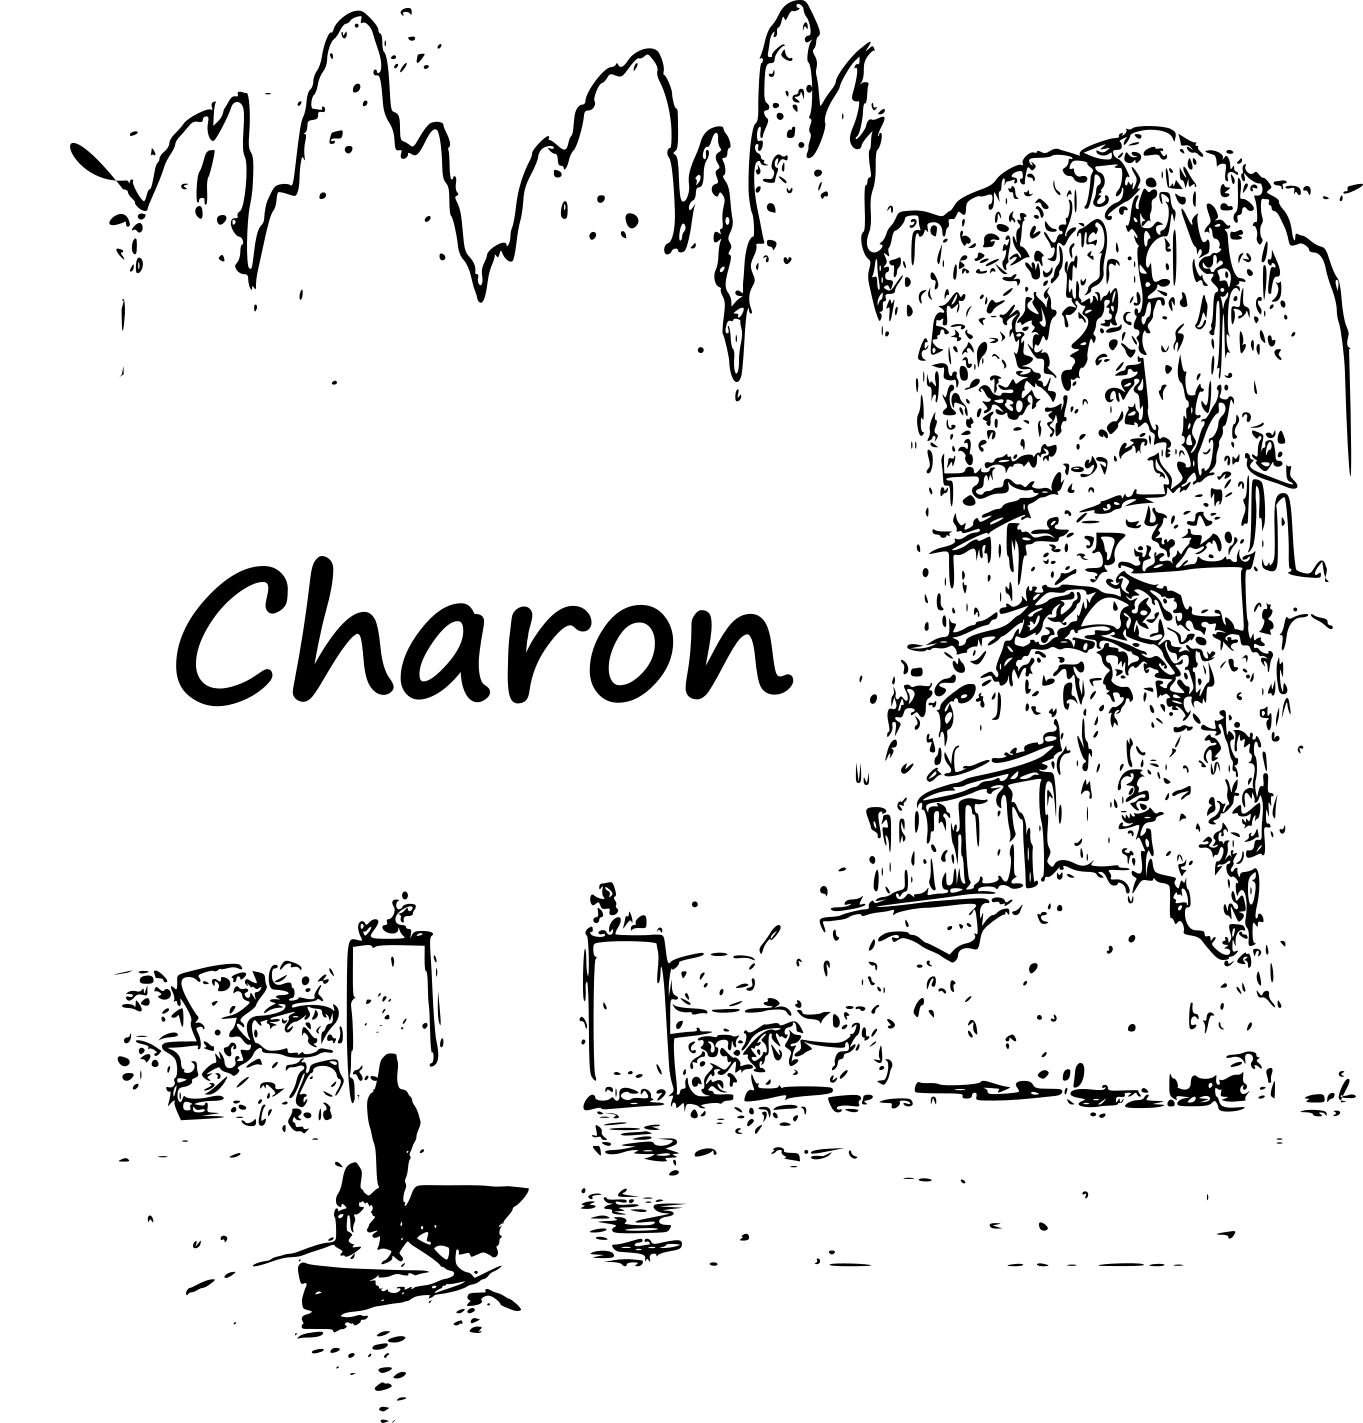
\includegraphics[width=0.8\textwidth]{\path/logo_Charon}
\end{figure}
\clearpage
\section{Installation de la librairie FEniCS}\label{Section:Installation de la librairie FEniCS CHARON}
Le code CHARON nécessite la librairie FEniCSx\footnote{\url{https://fenicsproject.org/documentation/}} laquelle peut s'installer de plusieurs façons\footnote{voir \url{https://github.com/FEniCS/dolfinx}}. Nous recommandons l'une des installations suivantes:
\begin{itemize}
\item Via le gestionnaire Anaconda\footnote{\url{https://anaconda.org/}} \subsecref{Subsection:Conda}, qui permet un meilleur cloisonnement par l'utilisation d'environnements virtuels. Notez que certaines extensions de FEniCSx ne sont facilement accessible que par conda, d'autres, au contraire, sont impossibles.
\item Sur Ubuntu, via le ppa \subsecref{Subsection:ppa}, qui permet l'installation du code \og en dur \fg{} sur toute la machine.
\item Via Spack ou Docker, cette solution est à privilégier sur les calculateurs  et permet en outre de bénéficier des version de développement de FEniCSx.
\end{itemize}
Si l'installation a lieu depuis la DIF, il peut être nécessaire d'insérer les lignes suivantes pour spécifier l'adresse du proxy :
\begin{equation}
\begin{aligned}
&\verb|export http_proxy=http://proxy.dam.intra.cea.fr:3128|\\
&\verb|export https_proxy=https://proxy.dam.intra.cea.fr:3128|
\end{aligned}
\label{export_proxy}
\end{equation}
Avec le mot clé \texttt{-E} après une commande \texttt{sudo}, l'opération s'effectuera au travers du proxy ci-dessus.
\subsection{Installation via Conda}\label{Subsection:Conda}
Après avoir exporté le proxy avec \eqref{export_proxy}, télécharger l'Anaconda installer:
\begin{verbatim}
sudo -E wget https://repo.anaconda.com/archive/Anaconda3-2024.02-1-Linux-x86\_64.sh
\end{verbatim}
Puis lancer l'installer avec
\begin{verbatim}
bash Anaconda3-2024.02-1-Linux-x86\_64.sh
\end{verbatim}
\begin{Rem}{Attention ne pas faire \texttt{sudo} ici sinon l'installation se fera sur le root.}\end{Rem}
Initialiser Anaconda
\begin{verbatim}
~anaconda3/bin/conda init
\end{verbatim}
Appliquer les changements:
\begin{verbatim}
source ~/.bashrc
\end{verbatim}
Vérifier la bonne installation de Conda en demandant la version:
\begin{verbatim}
conda --version
\end{verbatim}
Conda est maintenant normalement installé sur la machine, ensuite il est nécessaire de télécharger le package FEniCSx via le proxy. Pour cela:
\begin{verbatim}
conda config --set proxy_servers.http http://proxy.dam.intra.cea.fr:3128
conda config --set proxy_servers.https https://proxy.dam.intra.cea.fr:3128
conda create -n fenicsx-env
conda activate fenicsx-env
conda install -c conda-forge fenics-dolfinx mpich pyvista adios4dolfinx pyvista4dolfinx pytest 
\end{verbatim}
S'il y a un problème de proxy lors de la création de l'environnement il peut être utile de re-spécifier en dur l'adresse du proxy via :
\begin{verbatim}
conda create -n fenicsx-env --proxy http://proxy.dam.intra.cea.fr:3128
\end{verbatim}
Puis pour lancer un calcul ultérieurement il faut activer l'environnement en tapant :
\begin{verbatim}
conda activate fenicsx-env
\end{verbatim}
Pour vérifier quels sont les packages installer dans l'environnement virtuel créé par Anaconda il faut taper:
\subsection{Installation via ppa}\label{Subsection:ppa}
Dans un terminal, après avoir exporté le proxy avec \eqref{export_proxy} appliquer successivement les commandes:
\begin{verbatim}
sudo -E apt install software-properties-common
sudo -E add-apt-repository ppa:fenics-packages/fenics
sudo -E apt update
sudo -E apt upgrade
sudo -E apt install fenicsx
\end{verbatim}
Ces lignes de codes permettent à un utilisateur se trouvant sur le site du CEA-DAM de spécifier l'adresse du proxy puis d'installer la librairie FEniCS.

Afin de pouvoir profiter de toutes les options de Charon nous recommendons également l'installation des librairires suivantes:
\begin{verbatim}
sudo -E apt install python3-pip
sudo -E apt install spyder
sudo -E apt install paraview
sudo -E pip3 install --upgrade gmsh
sudo - E pip3 install jax jaxlib
sudo - E pip3 install diffrax
\end{verbatim}
\subsection{Problème lors de l'installation}
Si certains packages ont été incorrectement installés où sont présent en doublon (par exemple petsc4py qui aurait été installé préalablement via pip), nous conseillons de désinstaller les potentiels conflits (par exemple pip uninstall petsc4py) puis sudo apt autoremove fenicsx (et pas seulement remove qui n'enlèverait pas les dépendances).
\subsection{Désinstallation de FEniCSx}
Pour une désinstallation complète de FEniCSx (à cause d'une échec de mise à jour par exemple) il est possible d'effectuer successivement les commandes suivantes:
\begin{verbatim}
sudo apt remove --purge python3-ufl python3-dolfinx python3-ffcx
sudo apt autoremove
rm -rf ~/.cache/pip
sudo rm -rf /usr/lib/python3/dist-packages/ufl/__pycache__
sudo apt install fenicsx
\end{verbatim}
\section{Installation du code CHARON}
Après avoir naviguer jusque dans le dossier Charon, vérifier que le fichier \texttt{setup.py} s'y trouve, puis, dans un terminale de commande:
\begin{enumerate}
\item Si vous souhaitez réaliser du développement sur le code source, exécuter la commande:
\begin{equation}
\verb|sudo pip3 install --editable .|
\label{installation_avec_modifs}
\end{equation}
Cette commande va utiliser \texttt{pip3} pour installer CHARON comme un package classique et le rendre accessible où que se trouve votre fichier test. La commande \verb|--editable| spécifie que les modifications du code CHARON seront prises en compte lors de l'appel du package. Il est parfois nécessaire de fermer la console pour prendre en compte les ajustements.
\item Si vous ne souhaitez pas faire une quelconque modification sur CHARON, plutôt que d'installer le code en mode \og editable \fg{} avec la commande \eqref{installation_avec_modifs}, taper plutôt
\begin{verbatim}
sudo pip3 install .
\end{verbatim}
Et les modifications du code CHARON en local ne seront pas prises en compte lors de l’exécution.
\item Vérifier la correcte installation du package en tapant:
\begin{verbatim}
pip3 show Charon
\end{verbatim}
\end{enumerate}
Si l'utilisateur utilise Ubuntu 24.04 Noble Numbat sur lequel les installations globales ont été rendues plus sécurisées, il faut plutôt lancer les lignes de commandes suivantes:
\begin{verbatim}
sudo pip3 install --editable . --break-system-packages
\end{verbatim}
afin de forcer l'installation du paquet.
\subsection{Installation de CHARON via Conda}
Pour installer CHARON, aller simplement dans charonx-main et taper:
\begin{verbatim}
pip install --editable . 
\end{verbatim}
Par rapport à la commande \eqref{installation_avec_modifs} notons les différences suivantes:
\begin{itemize}
\item Pas besoin d'utiliser \texttt{sudo} car l'installation s'effectue dans un environnement Conda, pas au niveau système.
\item Utiliser simplement pip au lieu de pip3. Dans un environnement Conda, pip pointera automatiquement vers la version de Python de cet environnement.
\end{itemize}
Comme précédemment, l'option \verb|--editable| (ou \texttt{-e}) installera le package en mode développement, ce qui signifie que les modifications que vous apporterez au code source seront immédiatement reflétées sans avoir besoin de réinstaller le package.
\subsection{Utilisation d'un environnement virtuel avec CONDA}
Le problème majeur rencontré précédemment avec conda était l'impossibilité d'utiliser un editeur de texte tel que spyder à moins de l'installer directement dans l'environnement virtuel conda. Il est pourtant possible de le faire en utilisant l’interpréteur python qui se trouve à l'intérieur de l'environnement. Pour cela :
\begin{center}
\begin{verbatim}
conda activate fenicsx-env
which python
\end{verbatim}
\end{center}
Pour utiliser un environnement Conda spécifique dans Spyder:
\begin{enumerate}
    \item Ouvrir Spyder
    \item Aller dans Tools $\rightarrow$ Preferences $\rightarrow$ Python interpreter
    \item Sélectionner "Use the following Python interpreter"
    \item Spécifier le chemin de l'interpréteur Python de l'environnement souhaité (par exemple /home/bouteillerp/miniconda3/envs/fenicsx-env/bin/python)
    \item Fermer spyder et le relancer
\end{enumerate}
Il pourra vous être demandé d'installer un package supplémentaire dans conda tel que
\begin{verbatim}
conda install spyder-kernels=2.5
\end{verbatim}
Puis dans la console spyder vous pouvez voir éventuellement si des packages extérieurs à l'environnement sont utilisable par exemple via:

\section*{Point de départ}
Bien que non obligatoire, une connaissance sommaire de FEniCSx et de sa syntaxe constitue un gain de temps appréciable pour la prise en main de CHARON.
\begin{itemize}[label=$\star$]
\item Le livre officiel de FEniCSx introduit, par l'intermédiaire d'exemples multiphysiques variés l'implémentation de la résolution d'une équation aux dérivées partielles avec FEniCS. Il est disponible à l'adresse suivante:
\begin{center}
\url{https://fenicsproject.org/book/}
\end{center}
\item Le projet COMET constitue également une excellente introduction à FEniCS, ses composantes et son application à la mécanique du solide. Il peut être consulté via:
\begin{center}
\url{https://bleyerj.github.io/comet-fenicsx/index.html}
\end{center}
\item La page de Corrado-Maurini
\begin{center}
\url{http://www.lmm.jussieu.fr/~corrado/_site/codes/}
\end{center}
\item Les tutoriels associés à FEniCSx ont une porté plus large et présente aussi bien des problèmes de mécaniques des fluides, du solide, d'éléctromagnétisme que des cas test purement mathématiques. Ils sont plus avancés et sont accessibles à l'adresse suivante:
\begin{center}
\url{https://jsdokken.com/dolfinx-tutorial/}
\end{center}
\begin{center}
\url{https://docs.fenicsproject.org/dolfinx/v0.6.0/python/demos.html#advanced-demos}
\end{center}
\item Pour les utilisateurs avertis qui souhaiteraient développer leurs propres éléments ou des règles de quadrature spécifiques, nous renvoyons vers la page de tutoriels de Basix:
\begin{center}
\url{https://docs.fenicsproject.org/basix/main/python/demo/index.html}
\end{center}
\item Pour les utilisateurs souhaitant en savoir plus sur l’interfaçage entre gmsh et dolfinx:
\begin{center}
\url{https://jsdokken.com/src/tutorial_gmsh.html}
\end{center}
\end{itemize}
\section*{Feuille de route}
Le code CHARON est en cours de développement et ambitionne progressivement à incorporer les avancées suivantes:
\begin{itemize}
\item Méthode de remaillage adaptative grâce à gmsh
\item Ajout du contact:
\begin{center}
\url{https://github.com/Wells-Group/asimov-contact/tree/main/python}
\end{center}
\item Ajout des external Operator
\begin{center}
\url{https://orbilu.uni.lu/handle/10993/60511}
\end{center}
\end{itemize}
\part{Pratique}\label{Part:Pratique}
\chapter{Exemples concrets d'utilisation}\label{Chapitre:Exemples concrets}
Ce premier chapitre est consacré à la prise en main de CHARON par l'exemple. Seuls les fichiers d'input sont présentés et commentés; CHARON agit comme une boite noire. Un prochain chapitre introduira plus finement la structure du code et précisera les modifications que l'utilisateur peut apporter.

Les sections à suivre possèdent la même structure, nous commentons, étape par étape, les phases de construction du modèle.

\begin{itemize}[label = $\star$]
\item Le premier exemple, \secref{Section:Traction élastique quasi-statique d'un barreau 1D}, aborde la traction d'un barreau obéissant à la loi de Hooke. Le milieu est unidimensionnel en géométrie cartésienne.
\item Le deuxième exemple, \secref{Section:Compression dynamique d'une sphère creuse}, aborde la propagation d'une onde de compression dans une sphère creuse. L'élasticité obéit à une loi en grandes transformations.
\item Le troisième exemple, \secref{Section:Diffusion thermique 1D}, traite de la diffusion de la chaleur avec validation analytique.
\item Le quatrième exemple, \secref{Section:Plasticité - Sphère creuse élasto-plastique}, examine le comportement élasto-plastique d'une sphère sous pression.
\item Le cinquième exemple, \secref{Section:Propagation d'onde dans un bi-matériau}, étudie la propagation d'ondes à travers une interface entre deux matériaux.
\end{itemize}

L'objectif de ce chapitre est d'illustrer le fonctionnement de CHARON par l'intermédiaire d'exemples variés. L'utilisateur souhaitant créer son propre code pourra alors copier les différents blocs élémentaires présentés ici pour créer son fichier d'entrée.

Sans entrer dans les détails un script d'entrée de Charon comporte 4 grandes étapes:
\begin{enumerate}
\item La définition du matériau au travers de la classe Material. C'est ici que l'utilisateur précisera le comportement déviatorique ainsi que l'équation d'état du matériau.
\item La définition du maillage avec l'appel de la classe MeshManager. L'utilisateur spécifiera les éventuelles marqueurs délimitant les conditions aux limites.
\item La création d'une instance de la classe Problem qui générera toutes les équations de la mécanique à résoudre notamment la formulation variationnelle et la loi de comportement.
\item La création d'un solver prenant en argument le problème précédemment défini.
\end{enumerate}
\clearpage
\section{Traction élastique quasi-statique d'un barreau 1D}\label{Section:Traction élastique quasi-statique d'un barreau 1D}

\begin{figure}[h!]
\centering 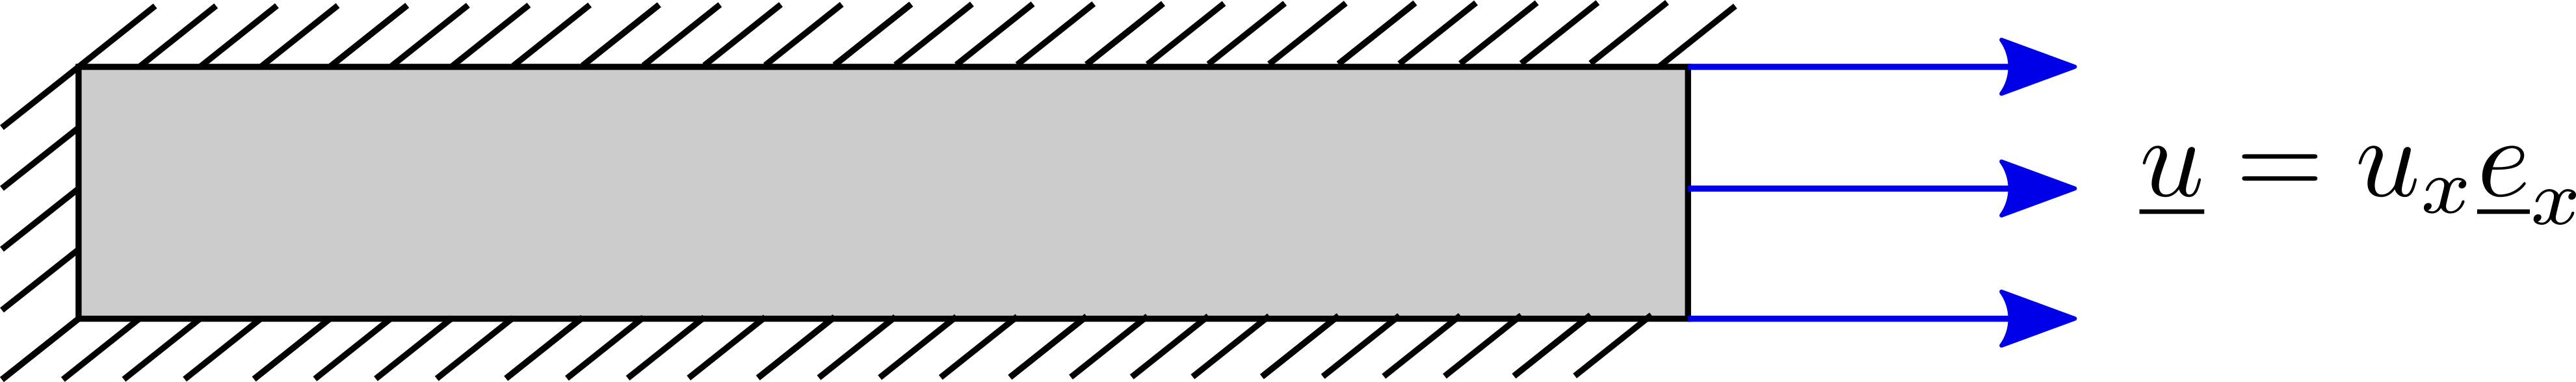
\includegraphics[width=0.8\textwidth]{\path/1D_Traction_schema}
\caption{Schéma de la traction unidimensionnelle.}
\label{fig:traction_1D_schema}
\end{figure}

\paragraph{Import du package} Un script débute nécessairement par l'importation du package Charon réalisé avec les ligne suivante:

\begin{figure}[h!]
\lstinputlisting[language=python,firstline=1, lastline=1]{Exemples_python_notice/1_Traction_1D_cartesien.py}
\end{figure}

Si les commandes d'installation du \chapref{Chapitre:Introduction} introductif ont été respectées, Charon est un package Python visible quel que soit l'emplacement du fichier d'entrée.

Tous les packages additionnels, par exemple \texttt{pandas} pour la lecture des résultats exportés au format \texttt{.csv}. ou \texttt{matplotlib} pour la visualisation des résultats doivent également être chargés ici.
\paragraph{Définition du modèle de comportement élastique} Après l'import des packages nécessaires, nous définissons le matériau qui est à l'étude lors de la simulation. 

Si l'utilisateur défini plusieurs matériaux et les stocke dans une liste, Charon comprendra qu'il s'agit d'une simulation multiphasique et des paramètres supplémentaires seront requis par l'analyse (comme la distribution spatiale des différents matériaux ou leurs capacités à évoluer de l'un vers l'autre). Toutes ces considérations sont reportées à l'exemple EXEMPLEREF.

Pour l'instant, nous renseignons les paramètres \emph{élastiques} nécessaires à la création du matériau d'étude.

\begin{figure}[h!]
\lstinputlisting[language=python,firstline=2, lastline=13]{Exemples_python_notice/1_Traction_1D_cartesien.py}
\end{figure}
Définir un matériau nécessite 6 paramètres:
\begin{enumerate}
\item Une masse volumique initiale $\rho_{0}$
\item Une capacité thermique massique initiale $C_{\mathrm{mass}}$
\item Une chaîne de caractère correspondant au nom de l'équation d'état retenu. Actuellement les chaines de caractères possibles sont:
\begin{center}
\keyword{IsotropicHPP}, \keyword{U1}, \keyword{U5}, \keyword{U8}, \keyword{Vinet}, \keyword{MG}, \keyword{JWL}, \keyword{MACAW}, \keyword{Tabulated}
\end{center}
Nous conseillons à l'utilisateur à se reporter à la partie théorie pour voir l'expression de la pression en fonction de la massique volumique et de la température associée à chacun de ces modèles.
\item Une chaine de caractère donnant le comportement déviatorique. Les mots clés actuellement disponible sont:
\begin{center}
\keyword{IsotropicHPP}, \keyword{NeoHook}, \keyword{MooneyRivlin}, \orange{None}
\end{center}
\item Un dictionnaire donnant les paramètres requis pour l'équation d'état. Il est crucial de noter que chaque équation d'état attend un nombre de paramètres fixés. Nous conseillons donc à l'utilisateur d'aller voir dans le code correspondant les paramètres requis. Si les paramètres ne sont pas correctement renseignés Charon renverra un message d'erreur indiquant les paramètres manquant.
\item Enfin, de même un dictionnaire précisant les paramètres requis à la définition de la loi déviatorique.
\end{enumerate}
Dans l'exemple ci-dessus, nous avons renseigné un module de Young $E=210 \times 10^3 \mega\pascal$, un coefficient de Poisson $\nu=0.3$, une masse volumique $\rho = 7.8 \times 10^{-3} \ton.\milli\metre^{-3}$, et une capacité thermique massique $C=500 \milli\metre^{2}.\second^{-2}.\kelvin^{-1}$. Ces ordres de grandeur correspondent à un acier standard METTRE REF Rajouter ref Salencon thermoélasticité.

Une loi d'état de type \keyword{IsotropicHPP} nécessite la donnée d'un module d'Young $E$, d'un coefficient de Poisson $\nu$ et d'un coefficient d'expansion thermique $\alpha$.

\paragraph{Paramètres géométriques, création du maillage et gestion des frontières} Pour construire notre maillage plusieurs options s'offrent à l'utilisateur. 
\begin{itemize}
\item Utiliser les fonctions de création de maillage propre à FEniCSx, auquel cas nous conseillons à l'utilisateur d'aller voir la page associée\footnote{\url{https://docs.fenicsproject.org/dolfinx/main/python/generated/dolfinx.mesh.html}}. Cette option permet la création de maillages simples: segment, rectangle ou pavé droit.
\item Utiliser un mailleur externe interfaçable avec FEniCSx par exemple gmsh\footnote{\url{https://gmsh.info/}}. De nombreux exemples sont disponibles avec une recherche internet.
\item L'utilisation d'un maillage abstrait, depuis la version Charon offre la possibilité de définir le problème posé sur un maillage abstrait afin d’accélérer le processus de remaillage pendant la simulation de dynamique explicite.
\end{itemize}
\begin{figure}[h!]
\lstinputlisting[language=python,firstline=15, lastline=20]{Exemples_python_notice/1_Traction_1D_cartesien.py}
\end{figure}
EN plus du maillage le constructeur MeshManager attend un dictionnaire permettant de marquer les frontières. Deux possibilités s'offrent à l'utilisateur:
\begin{itemize}
\item De marquer les frontières grâce aux outils internes de Charon, auquel cas il faudra placer trois mots clés : \keyword{tags}, \keyword{coordinate}, \keyword{position}. Ce constructeur est simple. Dans l'exemple ci-dessous il affecte le drapeau $1$ à tous les points du maillage tel que $x=0$ et le drapeau 2 à tous les points du maillage tels que $x=\text{Longueur}$.
\item Si le maillage a été généré par gmsh, il est possible de lui donner directement les facets\_tags, autrement dit les zones marqués dans gmsh. Cette option est illustrée dans l'exemple EXEMPLEREF
\end{itemize}
Ici, la barre à l'étude sera de longueur $L=1\milli\metre$, discrétisé avec deux éléments et ses extrémités seront marqués avec les drapeaux 1 et 2.


\paragraph{Définition des conditions aux limites} Nous souhaitons appliquer un déplacement $U_{max}=1 \times 10^{-3}\milli\metre$ à l'extrémité droite de la bare. Pour cela, nous définissant un objet de la classe \purple{MyConstant}
\begin{figure}[h!]
\lstinputlisting[language=python,firstline=23, lastline=24]{Exemples_python_notice/1_Traction_1D_cartesien.py}
\end{figure}

La classe \purple{MyConstant} permet de créer des conditions aux limites simples. Les types disponibles sont:
\begin{center}
\keyword{Creneau}, \keyword{SmoothCreneau}, \keyword{Chapeau}, \keyword{Rampe}, \keyword{UserDefined}
\end{center}
et les paramètres nécessaires 
\paragraph{Dictionnaire du problème} Un problème mécanique est une instance d'une des classes suivantes :
\begin{itemize}
\item \purple{CartesianUD}, modèle 1D cartésien,
\item \purple{CylindricalUD}, modèle 1D cylindrique,
\item \purple{SphericalUD}, modèle 1D sphérique,
\item \purple{PlaneStrain}, modèle 2D cartésien (déformation plane),
\item \purple{Axisymmetric}, modèle 2D axisymétrique,
\item \purple{Tridimensional}, modèle 3D complet.
\end{itemize}
Toutes ces classes prennent en argument un matériau (ou une liste de matériau dans un cas multiphasique) et un dictionnaire de paramètres. Nous détaillons ici tous les paramètres accessibles.
\begin{itemize}
\item Le premier argument consiste à donner l'objet mesh manager précédemment créé,
\item Le deuxième (Optionnel) contiens les conditions aux limites. A partir des drapeaux défini dans le mesh\_manager l'utilisateur va définir des conditions en limites en déplacement. Pour les conditions aux limites, les composantes disponibles selon le modèle sont:
\begin{itemize}
\item Modèles 1D: \keyword{U}
\item Modèles 2D plan: \keyword{Ux}, \keyword{Uy}
\item Modèles 2D axisymétrique: \keyword{Ur}, \keyword{Uz}
\item Modèles 3D: \keyword{Ux}, \keyword{Uy}, \keyword{Uz}
\end{itemize}
\item Le type d'analyse
\end{itemize}

\begin{figure}[h!]
\begin{lstlisting}[language=python]
# Configuration du problème
dictionnaire = {
   "mesh_manager": mesh_manager,
   "boundary_conditions": [
       {"component": "U", "tag": 1},                          # Blocage à gauche
       {"component": "U", "tag": 2, "value": chargement}      # Déplacement imposé à droite
   ],
   "analysis": "static",    # Type d'analyse
   "isotherm": True        # Calcul isotherme
}
\end{lstlisting}
\end{figure}

Les options pour le type d'analyse sont:
\begin{itemize}
\item \keyword{static}: analyse statique
\item \keyword{explicit\_dynamic}: analyse dynamique explicite (défaut)
\item \keyword{Pure\_diffusion}: diffusion thermique pure
\end{itemize}


\paragraph{Définition du modèle géométrique} La variable de modèle doit prendre ses valeurs parmi les mots clés suivants:



Il est absolument nécessaire que le maillage fourni soit cohérent avec le modèle. Ici, nous retenons un modèle simple 1D cartésien.

\paragraph{Résolution du problème}

\begin{figure}[h!]
\begin{lstlisting}[language=python]
# Création du problème
pb = CartesianUD(Acier, dictionnaire)

# Configuration de la résolution et des sorties
dictionnaire_solve = {
   "Prefix": "Traction_1D",
   "output": {"U": True},
   "csv_output": {"U": ["Boundary", 2]}
}

solve_instance = Solve(pb, dictionnaire_solve, compteur=1, npas=10)
solve_instance.solve()
\end{lstlisting}
\end{figure}

Les options de sortie disponibles sont:
\begin{itemize}
\item \keyword{U}: champ de déplacement
\item \keyword{v}: champ de vitesse
\item \keyword{Sig}: champ des contraintes
\item \keyword{Pressure}: champ de pression
\item \keyword{T}: champ de température
\item \keyword{deviateur}: déviateur des contraintes
\end{itemize}

\clearpage

\section{Compression dynamique d'une sphère creuse}\label{Section:Compression dynamique d'une sphère creuse}

\paragraph{Paramètres du problème} Pour cet exemple dynamique, nous étudions une sphère creuse soumise à une pression externe:

\begin{figure}[h!]
\begin{lstlisting}[language=python]
from Charon import SphericalUD, create_interval, MeshManager
from mpi4py.MPI import COMM_WORLD

# Paramètres géométriques
e = 5              # Épaisseur
R_int = 5          # Rayon interne
R_ext = R_int + e  # Rayon externe
Pext = 10          # Pression appliquée (MPa)

# Paramètres temporels
Tfin = 3e-4        # Temps de simulation (ms)
pas_de_temps = Tfin / 10000
magnitude = 1e4    # Amplitude du chargement
\end{lstlisting}
\end{figure}

\paragraph{Configuration du modèle sphérique}

\begin{figure}[h!]
\begin{lstlisting}[language=python]
# Création du maillage sphérique 1D (radial)
Nx = 2000
mesh = create_interval(COMM_WORLD, Nx, 
                     [np.array(R_int), np.array(R_ext)])

# Configuration du gestionnaire de maillage
dictionnaire_mesh = {
   "tags": [1, 2], 
   "coordinate": ["r", "r"], 
   "positions": [R_int, R_ext]
}
mesh_manager = MeshManager(mesh, dictionnaire_mesh)

# Chargement en créneau
chargement = MyConstant(mesh, Tfin, magnitude, Type="Creneau")
\end{lstlisting}
\end{figure}

\paragraph{Conditions aux limites et résolution dynamique}

\begin{figure}[h!]
\begin{lstlisting}[language=python]
# Configuration du problème dynamique
dictionnaire = {
   "mesh_manager": mesh_manager,
   "loading_conditions": [
       {"type": "surfacique", "component": "F", 
        "tag": 2, "value": chargement}
   ],
   "isotherm": True
}

# Création du problème sphérique
pb = SphericalUD(Acier, dictionnaire)

# Résolution dynamique explicite
dictionnaire_solve = {
   "Prefix": "Compression_spherique",
   "csv_output": {"Sig": True}
}

solve_instance = Solve(pb, dictionnaire_solve, 
                     compteur=500, TFin=Tfin, 
                     scheme="fixed", dt=pas_de_temps)
solve_instance.solve()
\end{lstlisting}
\end{figure}

Les types de conditions de chargement disponibles sont:
\begin{itemize}
\item \keyword{surfacique}: force surfacique appliquée
\item \keyword{volumique}: force volumique appliquée
\item \keyword{pressure}: pression (pour modèles axisymétriques)
\end{itemize}

Les composantes de force selon le modèle:
\begin{itemize}
\item Modèles 1D: \keyword{F}
\item Modèles 2D plan: \keyword{Fx}, \keyword{Fy}
\item Modèles 2D axisymétrique: \keyword{Fr}, \keyword{Fz}, \keyword{pressure}
\item Modèles 3D: \keyword{Fx}, \keyword{Fy}, \keyword{Fz}
\end{itemize}

\clearpage

\section{Diffusion thermique 1D}\label{Section:Diffusion thermique 1D}

\paragraph{Configuration du problème de diffusion}

\begin{figure}[h!]
\begin{lstlisting}[language=python]
from Charon import LinearThermal
from ufl import conditional, SpatialCoordinate, And, lt, gt
from dolfinx.fem import Expression, Function

# Matériau thermique
lmbda_diff = 240e-3  # Conductivite thermique (W/(mm\cdot K))
AcierTherm = LinearThermal(lmbda_diff)

# Parametres geometriques
L = 210e-3           # Longueur totale
bord_gauche = -105e-3
bord_droit = bord_gauche + L
point_gauche = -5e-3  # Limite gauche de la zone chaude
point_droit = 5e-3    # Limite droite de la zone chaude

# Températures
Tfroid = 300         # Température froide (K)
TChaud = 800         # Température chaude (K)

# Paramètres temporels
Tfin = 1e-3          # Temps final (ms)
pas_de_temps = 5e-6  # Pas de temps (ms)
Nx = 1000           # Nombre d'éléments
\end{lstlisting}
\end{figure}

\paragraph{Conditions initiales et résolution}

\begin{figure}[h!]
\begin{lstlisting}[language=python]
# Création du maillage
mesh = create_interval(COMM_WORLD, Nx, 
                     [np.array(bord_gauche), np.array(bord_droit)])

dictionnaire_mesh = {
   "tags": [1, 2], 
   "coordinate": ["x", "x"], 
   "positions": [bord_gauche, bord_droit]
}
mesh_manager = MeshManager(mesh, dictionnaire_mesh)

# Configuration pour diffusion pure
dictionnaire = {
   "mesh_manager": mesh_manager,
   "Thermal_material": AcierTherm, 
   "analysis": "Pure_diffusion"
}

pb = CartesianUD(Acier, dictionnaire)

# Définition de la température initiale avec condition UFL
x = SpatialCoordinate(mesh)
ufl_condition = conditional(
   And(lt(x[0], point_droit), gt(x[0], point_gauche)), 
   TChaud, Tfroid
)
T_expr = Expression(ufl_condition, pb.V_T.element.interpolation_points())

# Application de la condition initiale
pb.T0 = Function(pb.V_T)
pb.T0.interpolate(T_expr)
pb.T.interpolate(T_expr)
pb.bcs_T = []  # Pas de conditions aux limites thermiques

# Résolution
solve_instance = Solve(pb, {}, compteur=25, TFin=Tfin, 
                     scheme="fixed", dt=pas_de_temps)
solve_instance.solve()
\end{lstlisting}
\end{figure}

Les opérateurs UFL disponibles pour les conditions:
\begin{itemize}
\item \red{lt}: lower than (<)
\item \red{gt}: greater than (>)
\item \red{And}: et logique
\item \red{Or}: ou logique
\item \red{conditional}: condition ternaire
\end{itemize}

\clearpage

\section{Plasticité - Sphère creuse élasto-plastique}\label{Section:Plasticité - Sphère creuse élasto-plastique}

\paragraph{Configuration du modèle plastique}

\begin{figure}[h!]
\begin{lstlisting}[language=python]
# Paramètres de plasticité
sig0 = 300          # Limite d'élasticité (MPa)
Et = E / 100.0      # Module tangent
H = E * Et / (E - Et)  # Module d'écrouissage

# Dictionnaire de plasticité
plasticity_dic = {
   "model": "HPP_Plasticity",        # ou "Finite_Plasticity"
   "sigY": sig0,                     # Limite élastique
   "Hardening": "Isotropic",         # Type d'écrouissage
   "Hardening_modulus": H            # Module d'écrouissage
}
\end{lstlisting}
\end{figure}

Les modèles de plasticité disponibles sont:
\begin{itemize}
\item \keyword{HPP\_Plasticity}: plasticité en petites perturbations
\item \keyword{Finite\_Plasticity}: plasticité en grandes transformations
\item \keyword{J2\_JAX}: modèle J2 avec JAX (écrouissage non-linéaire)
\end{itemize}

Les types d'écrouissage disponibles:
\begin{itemize}
\item \keyword{Isotropic}: écrouissage isotrope
\item \keyword{Kinematic}: écrouissage cinématique
\item \keyword{NonLinear}: écrouissage non-linéaire (avec fonction)
\end{itemize}

\paragraph{Configuration et résolution}

\begin{figure}[h!]
\begin{lstlisting}[language=python]
# Géométrie
Re = 600    # Rayon externe
Ri = 300.0  # Rayon interne
Nx = 50     # Nombre d'éléments

# Calcul de la pression limite élastique
q_lim = float(2 * np.log(Re / Ri) * sig0)
p_applied = 1.1 * q_lim  # 10% au-dessus de la limite

# Configuration du problème plastique
dictionnaire = {
   "mesh_manager": mesh_manager,
   "loading_conditions": [
       {"type": "surfacique", "component": "F", 
        "tag": 1, "value": p_applied}
   ],
   "analysis": "static",
   "plasticity": plasticity_dic,
   "isotherm": True
}

pb = SphericalUD(Acier, dictionnaire)

# Résolution avec nombreux pas pour convergence
solve_instance = Solve(pb, dictionnaire_solve, 
                     compteur=100, npas=20000)
solve_instance.solve()
\end{lstlisting}
\end{figure}

\clearpage

\section{Propagation d'onde dans un bi-matériau}\label{Section:Propagation d'onde dans un bi-matériau}

\paragraph{Configuration multi-matériau}

\begin{figure}[h!]
\begin{lstlisting}[language=python]
from Charon import Material
from ufl import SpatialCoordinate

# Définition de deux matériaux
# Matériau 1: Acier (déjà défini)
# Matériau 2: Aluminium
ratio = 3
E_alu = E / ratio
nu_alu = nu
rho_alu = 2.7e-3

dico_eos_alu = {"E": E_alu, "nu": nu_alu, "alpha": alpha}
dico_devia_alu = {"E": E_alu, "nu": nu_alu}

Alu = Material(rho_alu, C, "IsotropicHPP", "IsotropicHPP", 
              dico_eos_alu, dico_devia_alu)

# Liste des matériaux
Mat_list = [Acier, Alu]
\end{lstlisting}
\end{figure}

\paragraph{Configuration spatiale des phases}

\begin{figure}[h!]
\begin{lstlisting}[language=python]
# Paramètres géométriques
L = 50              # Longueur totale
demi_longueur = L/2 # Position de l'interface

# Définition des conditions spatiales pour chaque matériau
x = SpatialCoordinate(mesh)

dictionnaire = {
   "mesh_manager": mesh_manager,
   "boundary_conditions": [
       {"component": "U", "tag": 2}
   ],
   "loading_conditions": [
       {"type": "surfacique", "component": "F", 
        "tag": 1, "value": chargement}
   ],
   "multiphase": {
       "conditions": [x[0] < demi_longueur, x[0] >= demi_longueur]
   },
   "isotherm": True
}

# Création du problème multi-matériau
pb = CartesianUD(Mat_list, dictionnaire)
\end{lstlisting}
\end{figure}

Le mode multi-matériau est activé automatiquement lorsque:
\begin{itemize}
\item Le matériau passé en argument est une liste
\item Le dictionnaire contient une entrée \keyword{multiphase}
\item Les conditions spatiales sont définies via des expressions UFL
\end{itemize}

\paragraph{Options avancées}

\begin{figure}[h!]
\begin{lstlisting}[language=python]
# Configuration des paramètres FEM
dictionnaire_mesh = {
   "tags": [1, 2], 
   "coordinate": ["x", "x"], 
   "positions": [0, L],
   "fem_parameters": {
       "u_degree": 2,         # Degré des éléments
       "schema": "reduit"     # Intégration réduite
   }
}

# Configuration de l'amortissement
dictionnaire = {
   # ... autres paramètres
   "damping": {
       "damping": True,       # Activation de l'amortissement
       "linear_coeff": 0.1,   # Coefficient linéaire
       "quad_coeff": 0.01,    # Coefficient quadratique
       "correction": True     # Correction géométrique
   }
}
\end{lstlisting}
\end{figure}

Les options d'amortissement disponibles:
\begin{itemize}
\item \keyword{damping}: activation/désactivation
\item \blue{linear\_coeff}: coefficient d'amortissement linéaire
\item \blue{quad\_coeff}: coefficient d'amortissement quadratique
\item \keyword{correction}: prise en compte des changements de géométrie
\end{itemize}

\paragraph{Post-traitement et sorties}

\begin{figure}[h!]
\begin{lstlisting}[language=python]
# Configuration complète des sorties
dictionnaire_solve = {
   "Prefix": "Nom_simulation",
   "output": {
       "U": True,          # Déplacements (format XDMF)
       "v": True,          # Vitesses
       "Sig": True,        # Contraintes
       "Pressure": True    # Pression
   },
   "csv_output": {
       "U": ["Boundary", 1],     # Déplacements sur frontière 1
       "Sig": True,              # Contraintes aux points de Gauss
       "Pressure": True,         # Pression aux points de Gauss
       "deviateur": True         # Déviateur des contraintes
   }
}

# Fonction de post-traitement personnalisé
def query_output(problem, t):
   # Appelée à chaque pas de temps
   problem.eps_list.append(problem.current_strain)
   problem.F_list.append(problem.get_F(problem.Force))

def final_output(problem):
   # Appelée en fin de calcul
   import matplotlib.pyplot as plt
   plt.plot(problem.eps_list, problem.F_list)
   plt.show()

solve_instance = Solve(pb, dictionnaire_solve, compteur=100, npas=1000)
solve_instance.query_output = query_output
solve_instance.final_output = final_output
solve_instance.solve()
\end{lstlisting}
\end{figure}

Cette nouvelle interface de CHARON offre une approche plus moderne et flexible pour la définition des problèmes mécaniques, avec une séparation claire entre la définition des matériaux, du maillage, des conditions aux limites et de la résolution.
\chapter{Solutions analytiques}\label{Chapitre:Solutions analytiques}
Les solutions analytiques sont de rares et précieux résultats permettant la validation d'un modèle numérique. En mécanique du solide, à cause de la complexité, et des équations de comportement, et de la géométrie, de telles solutions sont souvent inaccessibles. Cependant, ce deuxième chapitre compile  quelques cas de figure simples où les calculs peuvent être achevés \og à la main \fg{}. Les résultats de CHARON sont alors comparés à ces solutions afin de valider l'implémentation du code.\\

Lorsqu'une fonction $f$ est connue analytiquement, nous comparerons sa valeur analytique $f_{\mathrm{theo}}$, à son pendant numérique $f_{\mathrm{num}}$, par l'intermédiaire du critère (arbitraire) suivant:
$$\varepsilon=\dfrac{\int |f_{\mathrm{num}}(x)-f_{\mathrm{theo}}(x)|\dx}{\int |f_{\mathrm{theo}}(x)|\dx}$$
Ou encore, étant donné les valeurs discrètes des fonctions $f_{\mathrm{num}}$ et $f_{\mathrm{theo}}$, toutes deux connues aux mêmes points $(x_{k})$:
$$\varepsilon=\dfrac{\sum_{k} |f_{\mathrm{num}}(x_{k})-f_{\mathrm{theo}}(x_{k})|}{\sum|f_{\mathrm{theo}}(x_{k})|}$$
Pour chaque test, nous fixerons \emph{a priori} un écart $\varepsilon$ \og acceptable \fg{}.\\


Afin de s'assurer du bon fonctionnement du code, nous conseillons aux utilisateurs d’exécuter périodiquement la commande
\begin{verbatim}
python3 -m pytest
\end{verbatim}
depuis le répertoire CHARON afin d’appeler l'ensemble des comparaisons analytique/numérique validant ainsi:
\begin{itemize}
\item L'installation de CHARON
\item La non-régression du code consécutive à un nouveau développement.
\end{itemize}
Dans tous les tests qui ne seront pas dédiés spécifiquement à la validation des équations d'état ou de loi de comportement déviatorique, le matériau d'étude correspondra à un acier standard :
\begin{equation}
\begin{aligned}
E &= 210\times 10^{3}\mega\pascal && \text{Module de Young}\\
\nu &= 0.3 && \text{Coefficient de Poisson}\\
\rho &= 7.8\times 10^{3}\kilo\gram.\metre^{-3} && \text{Masse volumique}\\
\end{aligned}
\label{eq:pte_acier_standard}
\end{equation}
\section{Elasto-statique}
Nous débutons par un certain nombre de vérifications en statique permettant de valider les matrices de rigidités associées aux différents modèles.
\subsection{0D Validation des lois de comportement}
Nous étudions la traction d'une barre dans le cadre d'une modélisation 1D Cartésien avec un unique élément à interpolation linéaire. En imposant le déplacement de chacune des extrémités, nous contraingons intégralement le champ de déplacement est contraint sous la forme $\Dep=u_{x}\ex=\varepsilon x \ex$ avec $\varepsilon = u_{x,x}$ la déformation uni-axiale.\\

Nous notons de plus $\J$ le jacobien de la transformation, $\CGG$ le tenseur de Cauchy-Green gauche et $\dev\CGG$ son déviateur. Ces grandeurs sont respectivement donnés par:
\begin{equation}
\J=1+\varepsilon;\quad \CGG = (1+\varepsilon)^{2}\ex\otimes\ex+(\ey\otimes\ey+\ez\otimes\ez); \quad \dev\CGG = \dfrac{2\varepsilon+\varepsilon^{2}}{3}\left(2\ex\otimes\ex-\ey\otimes\ey-\ez\otimes\ez\right)
\label{eq:JBDEVB_1D_Cartesien}
\end{equation}
Par ailleurs, la déformation linéarisée $\DefoHPP$ et son déviateur $\dev\DefoHPP$, égalisent:
$$\DefoHPP = \varepsilon\ex\otimes\ex; \quad \dev\DefoHPP = \dfrac{\varepsilon}{3}\left(2\ex\otimes\ex-\ey\otimes\ey-\ez\otimes\ez\right)$$
Selon l'équation d'état et le modèle déviatorique sélectionnés, nous pouvons en déduire l'expression de la contrainte tridimensionnelle. Les solutions pour tout une gamme d'équations d'états et de comportement déviatorique sont maintenant étudiées.
\subsubsection{Équations d'état} Le jacobien de la transformation est uniforme sur le barreau (voir \eqref{eq:JBDEVB_1D_Cartesien}) $\J=1+\varepsilon$. Suivant les équations d'états précisés à la \secref{Section:Loi d'état}, les pressions valent donc:
\begin{center}
\begin{tabular}{|c|c|c|c|}\hline
Modèle & $U_{1}$ & $U_{2}$ & $U_{3}$\\\hline
\widecellh{4.5}{3.5}{Pression} & $p_{1}(J)=-\BulkModulus(\J-1)$ & $p_{2}(J)=-\BulkModulus\dfrac{\ln (\J)}{\J}$ & $p_{3}(J)=\dfrac{1}{2}(p_{1}(J) + p_{2}(J))$ \\\hline
Modèle & $U_{5}$ & $U_{7}$ & $U_{8}$\\\hline
\widecellh{4.5}{3.5}{Pression} & $p_{5}(J)=-\BulkModulus\ln\J$ & $p_{7}(\J)=-\dfrac{\BulkModulus}{2}\left(\exp(J-1)-\dfrac{1}{J}\right)$ & $p_{8}(\J)=-\dfrac{\BulkModulus}{2}\left(\ln\J-\dfrac{1}{J}+1\right)$\\\hline
\end{tabular}
\end{center}
Mais aussi pour les modèles de Mie-Gruneisen, de JWL et de Vinet:
\begin{center}
\begin{tabular}{|c|l|l|l|}\hline
\widecellh{4.5}{3.5}{MG} \eqref{eq:PMG} & $p_{\text{MG}}(J)=C\mu+D\mu^{2}+S\mu^{3}$ avec $\mu = \dfrac{1}{\J}-1$\\\hline
\widecellh{4.5}{3.5}{JWL} \eqref{eq:loi_etat_JWL} & $p_{\text{JWL}}(\J)=A\exp(-R_{1}\J)+B\exp(-R_{2}\J)$\\\hline 
\widecellh{4.5}{3.5}{Vinet} \eqref{eq:eos_Vinet} & $p_{\text{Vinet}}(\J)=3K_{0}(T)\J^{-2/3}(1-\J^{1/3})e^{\frac{3}{2}(K_{1}(T)-1)(1-\J^{1/3})}$\\\hline
\end{tabular}
\end{center}
Pour la comparaison analytique numérique représentée à la \figref{fig:compa_eos}, nous prenons arbitrairement:
\begin{itemize}
\item $\BulkModulus = 1e^{4}$, pour le modèle $U_{8}$,
\item Pour le modèle JWL, afin d'assurer une pression nul à $\J=1$ et un module tangent égal à $\kappa$ au voisinage de $\J=1$, nos coefficients $A$, $B$, $R_{1}$, $R_{2}$ doivent satisfaire le système:
$$\left\{\begin{aligned}
&Ae^{-R_{1}}+Be^{-R_{2}}=0\\
&AR_{1}e^{-R_{1}}+BR_{2}e^{-R_{2}}=\BulkModulus\\
\end{aligned}\right. \equivalent \left\{\begin{aligned}
&e^{-R_{2}}=-\frac{Ae^{-R_{1}}}{B}\\
&AR_{1}e^{-R_{1}}-R_{2}Ae^{-R_{1}}=\BulkModulus\\
\end{aligned}\right.\equivalent 
\left\{\begin{aligned}
&B=-\frac{Ae^{-R_{1}}}{e^{-R_{2}}}\\
&R_{2}=R_{1}-\dfrac{\BulkModulus}{Ae^{-R_{1}}}\\
\end{aligned}\right.$$
Nous prenons par exemple $A = 40000$, $R_{1}=1.5$, $R_{2} = 0.38$, $B = -13046$.
\item Pour le modèle de Vinet, nous prenons $K_{0}=\BulkModulus$, $K_{1}=2$.
\item Pour le modèle de Mie-Gruneisen, nous prenons $C=\BulkModulus$, $D=10$, $S=100$.
\end{itemize}
\begin{figure}
\begin{subfigure}[b]{0.49\textwidth}
\centering 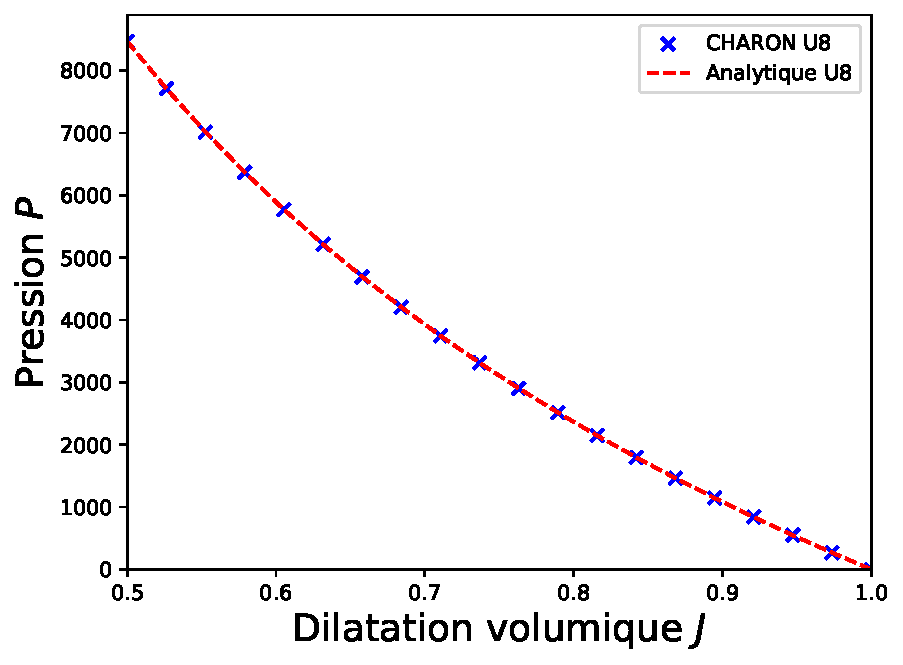
\includegraphics[width=0.98\textwidth]{\path/0DU8}
\caption{Loi $U_{8}$}
\label{fig:compa_U8}
\end{subfigure}
\begin{subfigure}[b]{0.49\textwidth}
\centering 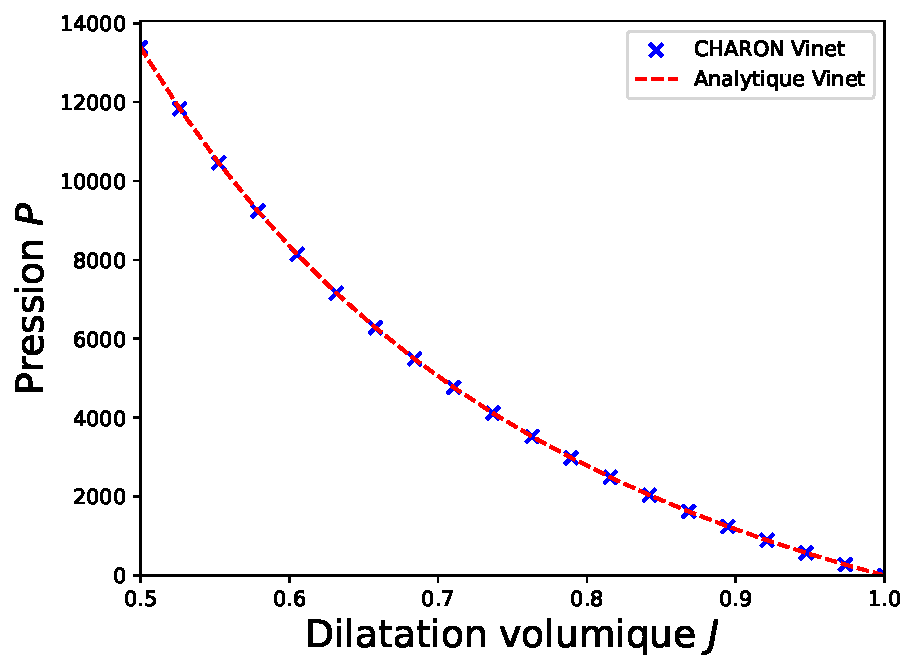
\includegraphics[width=0.98\textwidth]{\path/0DVinet}
\caption{Loi Vinet}
\label{fig:compa_Vinet}
\end{subfigure}
\begin{subfigure}[b]{0.49\textwidth}
\centering 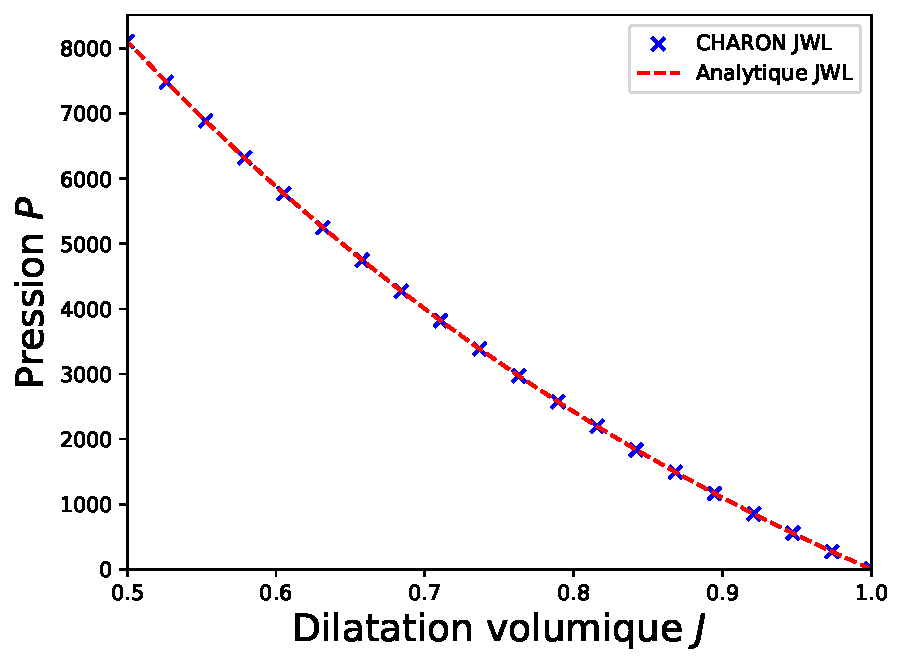
\includegraphics[width=0.98\textwidth]{\path/0DJWL}
\caption{Loi JWL}
\label{fig:compa_JWL}
\end{subfigure}
\begin{subfigure}[b]{0.49\textwidth}
\centering 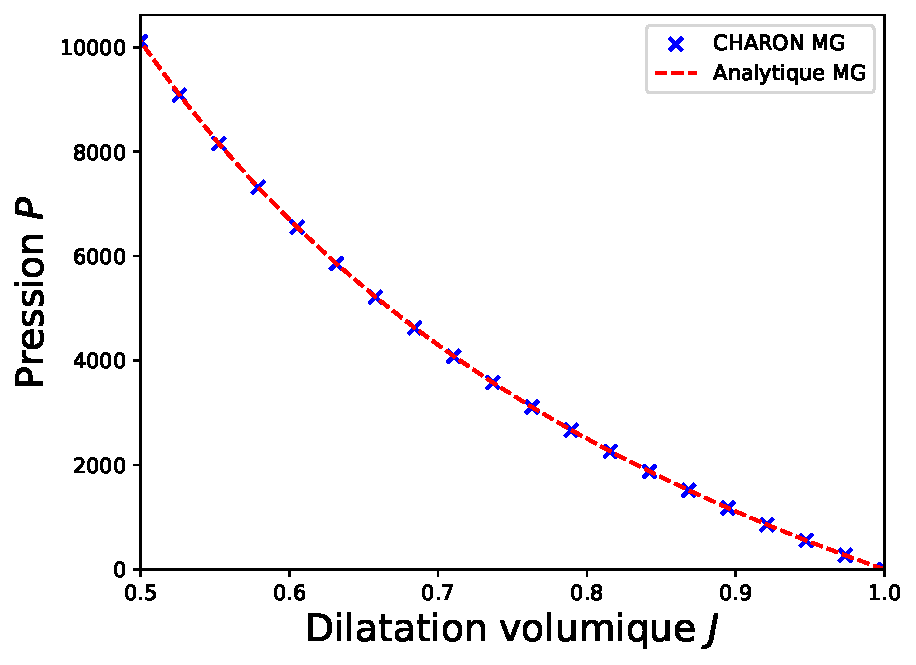
\includegraphics[width=0.98\textwidth]{\path/0DMG}
\caption{Loi Mie-Gruneisen}
\label{fig:compa_MG}
\end{subfigure}
\caption{Comparaison analytique numérique de quelques équations d'états.}
\label{fig:compa_eos}
\end{figure}
\FloatBarrier
\subsubsection{Loi de comportement déviatorique isotrope}
Puis nous procédons de même pour les déviateurs:
{\scriptsize
$$\begin{array}{rlcrl}
\CGG &= (1+\varepsilon)^{2}\ex\otimes\ex+(\ey\otimes\ey+\ez\otimes\ez)  && \CGG^{2} &= (1+\varepsilon)^{4}\ex\otimes\ex+(\ey\otimes\ey+\ez\otimes\ez)\\\\
\dfrac{1}{3}\tr\CGG &= 1+ \dfrac{2\varepsilon+\varepsilon^{2}}{3} && \dfrac{1}{3}\tr\CGG^{2} &= 1+ \dfrac{4\varepsilon + 6\varepsilon^{2} + 4\varepsilon^{3} + \varepsilon^{4}}{3}\\\\
\dev\CGG &= \dfrac{2\varepsilon+\varepsilon^{2}}{3}\left(2\ex\otimes\ex-\ey\otimes\ey-\ez\otimes\ez\right) && \dev\CGG^{2} &= \dfrac{4\varepsilon + 6\varepsilon^{2} + 4\varepsilon^{3} + \varepsilon^{4}}{3}\left(2\ex\otimes\ex-\ey\otimes\ey-\ez\otimes\ez\right)\\
\end{array}$$}
Dont nous déduisons pour le modèle de Mooney-Rivlin:
$$\begin{aligned}
\dev\CGG^{2}-\tr(\CGG)\dev\CGG &= \left(\dfrac{4\varepsilon + 6\varepsilon^{2} + 4\varepsilon^{3} + \varepsilon^{4}}{3} -\dfrac{(3+2\varepsilon+\varepsilon^{2})(2\varepsilon+\varepsilon^{2})}{3}\right)\left(2\ex\otimes\ex-\ey\otimes\ey-\ez\otimes\ez\right)\\
&= \left(\dfrac{4\varepsilon + 6\varepsilon^{2} + 4\varepsilon^{3} + \varepsilon^{4}-6\varepsilon-7\varepsilon^{2}-4\varepsilon^{3}-\varepsilon^{4}}{3}\right)\left(2\ex\otimes\ex-\ey\otimes\ey-\ez\otimes\ez\right)\\
&= -\dfrac{2\varepsilon + \varepsilon^{2}}{3}\left(2\ex\otimes\ex-\ey\otimes\ey-\ez\otimes\ez\right)
\end{aligned}$$
\begin{center}
\begin{tabular}{|c|l|l|l|}\hline
Modèle & HPP & NeoHookéen & Mooney-Rivlin\\\hline
\widecellh{4.5}{3.5}{$s_{xx}$} & $s_{xx}=\dfrac{4\mu\varepsilon}{3}$ & $s_{xx}=\dfrac{2\mu(2\varepsilon+\varepsilon^{2})}{3(1+\varepsilon)^{5/3}}$ & $s_{xx}=\dfrac{2(2\varepsilon+\varepsilon^{2})}{3}\left(\dfrac{C_{01}}{(1+\varepsilon)^{5/3}}+\dfrac{C_{10}}{(1+\varepsilon)^{7/3}}\right)$ \\\hline
\end{tabular}
\end{center}
Les composante $s_{xx}$ numérique et analytique sont comparées à la \figref{fig:compa_loi_dev_analytique}.
\begin{figure}[h!]
\begin{subfigure}[b]{0.32\textwidth}
\centering 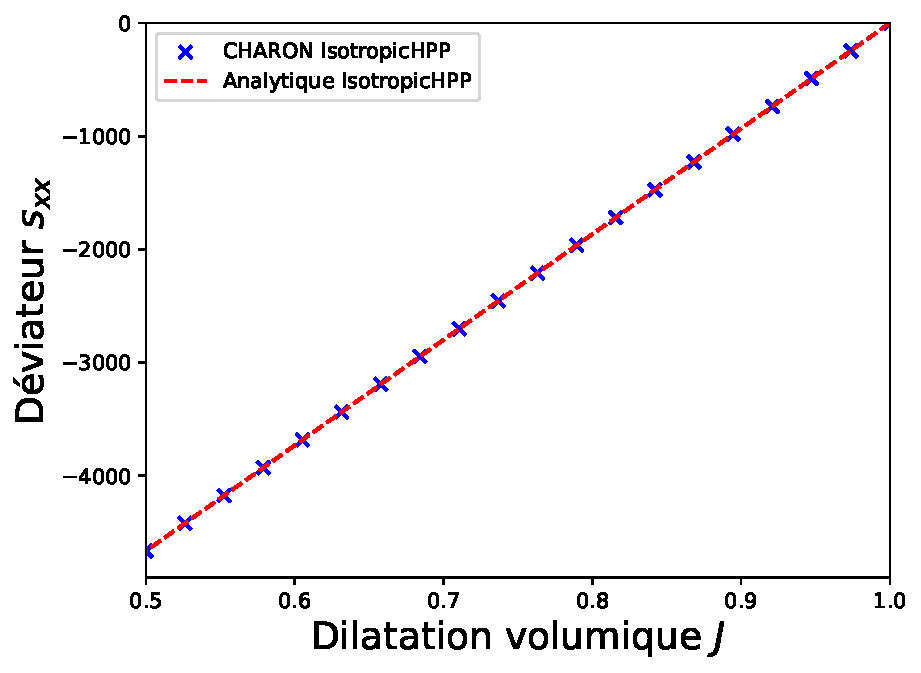
\includegraphics[width=\textwidth]{\path/0DIsotropicHPP}
\caption{Loi HPP}
\label{fig:compa_s_HPP}
\end{subfigure}
\begin{subfigure}[b]{0.32\textwidth}
\centering 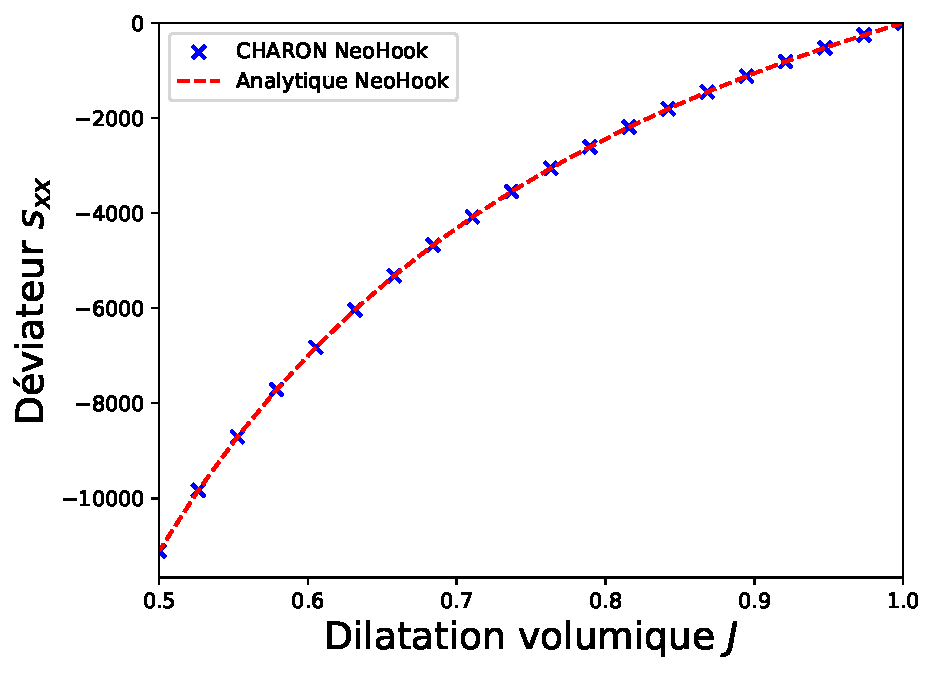
\includegraphics[width=\textwidth]{\path/0DNeoHook}
\caption{Loi Néo-Hookéenne}
\label{fig:compa_s_NH}
\end{subfigure}
\begin{subfigure}[b]{0.32\textwidth}
\centering 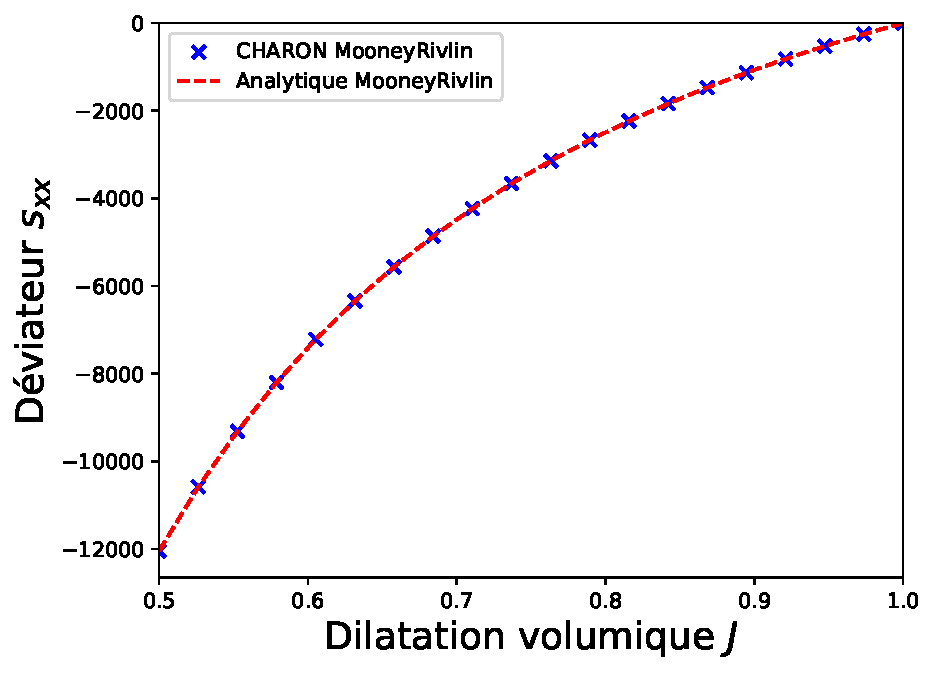
\includegraphics[width=\textwidth]{\path/0DMooneyRivlin}
\caption{Loi Mooney-Rivlin}
\label{fig:compa_s_MR}
\end{subfigure}
\caption{Comparaison analytique numérique de la loi de comportement déviatorique (ici $s_{xx}$).}
\label{fig:compa_loi_dev_analytique}
\end{figure}

\subsection{Essais 1D}
Nous mettons à l'épreuve nos modèles 1D Cartésien, cylindrique, sphérique.
\subsubsection{Traction uni-axiale en 1D}
Nous considérons un essai de traction simple avec le modèle 1D cartésien. Nous représentons à la \figref{fig:traction_1D_simple_HPP_Neo_Hook} la réaction associée à la condition aux limites en déplacement. Formellement le champ de contrainte est identique à celui du cas 0D et cet essai n'a d'autre intérêt que de valider l'implémentation lorsque le maillage est constitué de plusieurs éléments.
\subsubsection{Compression d'un cylindre sous pressions externe et interne}\label{Subsection:Compression d'un cylindre sous pressions externe et interne}
Nous considérons un cylindre soumis à une pression intérieure $p_{i}$ et à une pression extérieure $p_{e}$. Si le cylindre est constitué d'un matériau élastique linéaire isotrope, le champ de déplacement résultant est analytique (voir tableau p.284 \cite{forest2015mecanique}):
\begin{equation}
\Dep = \left(ar+\dfrac{b}{r}\right)\er+\left(cz+d\right)\ez
\label{eq:analytical_Ur_1D_cyl}
\end{equation}
et découle du champ de contrainte $\SC$ \eqref{eq:champ_contrainte_cyl_1D}
\begin{equation}
\SC = \left(A-\dfrac{B}{r^{2}}\right)\er\otimes\er+\left(1+\dfrac{B}{r^{2}}\right)\etheta\otimes\etheta+C\ez\otimes\ez
\label{eq:champ_contrainte_cyl_1D}
\end{equation}
Contrairement au champ de déplacement \eqref{eq:analytical_Ur_1D_cyl} issu de l'hypothèse d'élasticité linéarisée, le champ de contrainte \eqref{eq:champ_contrainte_cyl_1D} est indépendant de la loi de comportement retenue.\\

Dans ces expressions les constantes $A$, $B$, $C$, $a$, $b$, $c$ sont:
\begin{equation}
A=\dfrac{p_{i}r_{i}^{2}-p_{e}r_{e}^{2}}{r_{e}^{2}-r_{i}^{2}}; \quad B=\dfrac{p_{i}-p_{e}}{r_{e}^{2}-r_{i}^{2}}r_{e}^{2}r_{i}^{2}; \quad a=\dfrac{1-\nu}{E}A-\dfrac{\nu}{E}C; \quad b=\dfrac{B}{2\mu}; \quad c=\dfrac{1}{E}\left(C-2\nu A\right)
\label{eq:A_B_C_compression_cylindrique}
\end{equation}
La solution cylindrique 1D qui contraint le déplacement sous la forme $\Dep = u_{r}\er$ correspond au cas où le déplacement $u_{z}$ est bloqué aux deux extrémités du cylindre). Il convient par conséquent de retenir le cas \og $C=2\nu A$ \fg{} du tableau donné par Samuel Forest \cite{forest2015mecanique}.\\

Les paramètres numériques utilisés sont mentionnés dans le \Tableref{fig:compa_analytique_num_compr_cyl_1D}.
\begin{table}
\centering \begin{tabular}{llllll}\hline
$E(\mega\pascal)$  & $\nu$ & $r_{i}(\milli\metre)$ & $r_{e}(\milli\metre)$ & $p_{i}(\mega\pascal)$ & $p_{e}(\mega\pascal)$\\
$210\times10^{3}$ & 0.3 & $9$ & $11$ & $5$ & $10$\\\hline
\end{tabular}
\caption{Paramètres numériques pour la compression à symétrie cylindrique}
\label{fig:compa_analytique_num_compr_cyl_1D}
\end{table}
Nous représentons à la \figref{fig:compa_analytique_compr_cyl} les comparaisons entre les valeurs analytique et théorique concernant le champ de déplacement \eqref{eq:analytical_Ur_1D_cyl}.
\subsubsection{Compression d'une sphère sous pression externe}\label{Section:Compression d'une sphère sous pression externe}
Nous considérons une sphère soumise à une pression externe $p_{e}$. Les paramètres numériques utilisés sont identiques à ceux de la \subsecref{Subsection:Compression d'un cylindre sous pressions externe et interne}. La solution analytique de cet essai est détaillée dans:
\begin{center}
\url{https://comet-fenics.readthedocs.io/en/latest/demo/elasticity/axisymmetric_elasticity.html}
\end{center}
En raison de la symétrie du problème, une étude à symétrie sphérique 1D suffit. Nous validerons toutefois également l'implémentation du module axi-symétrique. Le champ de déplacement purement radial est donné par:
\begin{equation}
u_{r}(r)=-\dfrac{r_{e}^{3}}{r_{e}^{3}-r_{i}^{3}}\left((1-2\nu)r+(1+\nu)\dfrac{r_{i}^{3}}{2r^{2}}\right)\dfrac{p_{e}}{E}
\label{eq:solution_sphere_pression_externe}
\end{equation}
Si la sphère est chargée par une pression interne $p_{i}$ la solution est tout à fait analogue:
\begin{equation}
u_{r}(r)=\dfrac{r_{i}^{3}}{r_{e}^{3}-r_{i}^{3}}\left((1-2\nu)r+(1+\nu)\dfrac{r_{e}^{3}}{2r^{2}}\right)\dfrac{p_{i}}{E}
\label{eq:solution_sphere_pression_interne}
\end{equation}
Si la sphère est chargée à la fois par l'intérieure et par l'extérieure la solution est simplement, par linéarité, la superposition des deux champs de déplacements précédemment obtenus. Nous traçons l'évolution du déplacement radial en utilisant d'abord le modèle unidimensionnel sphérique. Le champ de déplacement pour $r\in[r_{i},r_{e}]$ est représenté \figref{fig:compa_analytique_compr_sph1D}.
\begin{figure}[h!]
\begin{subfigure}[b]{0.32\textwidth}
\centering 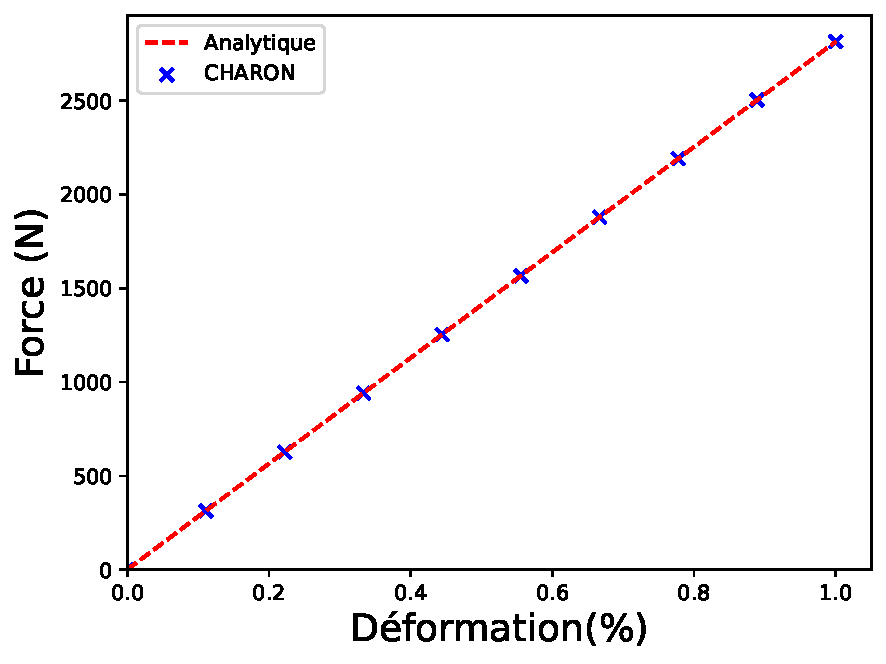
\includegraphics[width=1.02\textwidth]{\path/Traction_1DIsotropicHPPNeoHook}
\caption{Essai de traction 1D.}
\label{fig:traction_1D_simple_HPP_Neo_Hook}
\end{subfigure}\hfill
\begin{subfigure}[b]{0.32\textwidth}
\centering 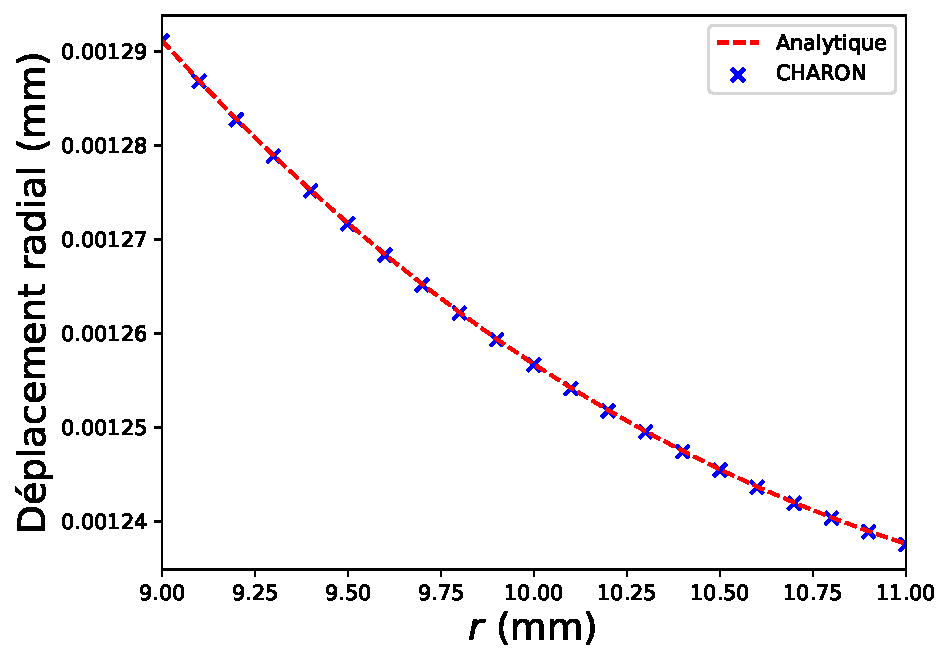
\includegraphics[width=1.1\textwidth]{\path/Cylindric_compression}
\caption{$u_{r}$, compression cylindrique.}
\label{fig:compa_analytique_compr_cyl}
\end{subfigure}\hfill
\begin{subfigure}[b]{0.32\textwidth}
\centering 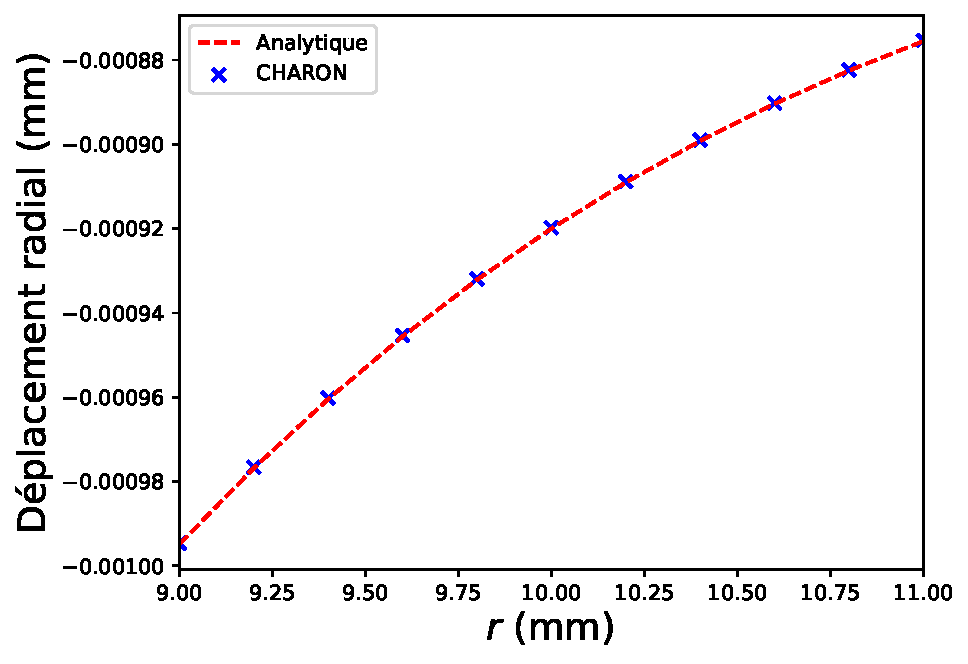
\includegraphics[width=1.1\textwidth]{\path/Spheric_compression}
\caption{$u_{r}$, compression sphérique}
\label{fig:compa_analytique_compr_sph1D}
\end{subfigure}
\caption{Comparaison analytique numérique 1D}
\end{figure}
\FloatBarrier
\subsubsection{Essai de traction sur un bi-matériau}
Nous étudions à présent la traction simple d'un barreau constitué de deux matériaux. L'un correspondant à un acier standard \eqref{eq:pte_acier_standard}, l'autre à un aluminium $E = 70\giga\pascal$.
\begin{figure}[h!]
\begin{subfigure}[b]{0.49\textwidth}
\centering 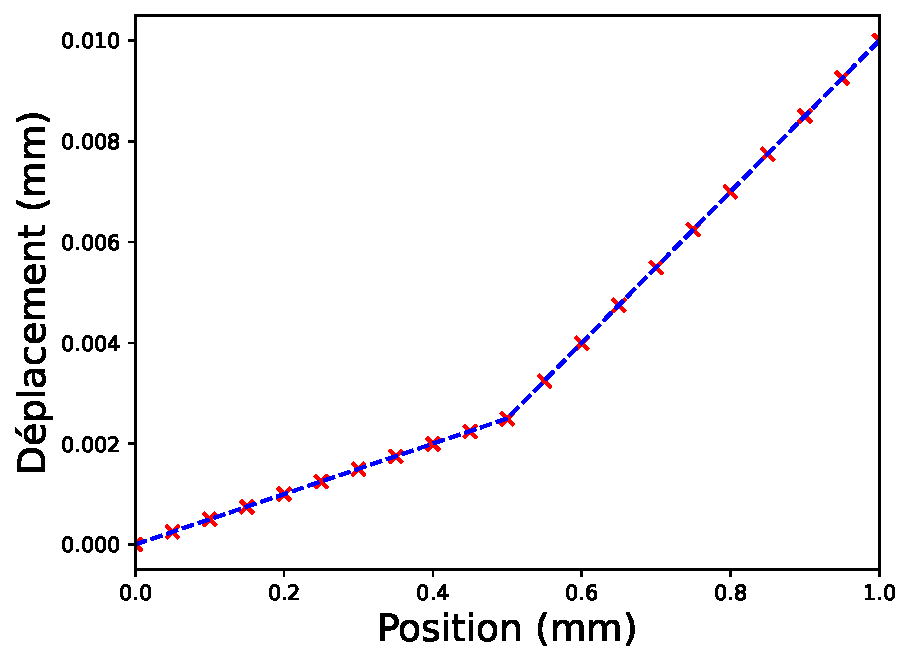
\includegraphics[width=\textwidth]{\path/Traction_bimat}
\caption{Déplacement bi-matériau}
\label{fig:compa_analytique_compr_sph1D}
\end{subfigure}\hfill
\begin{subfigure}[b]{0.49\textwidth}
\centering \includegraphics[width=\textwidth]{\path/1D_Traction_bimat}
\caption{Traction sur un bi-matériau.}
\label{fig:compa_analytique_num_bimat_traction}
\end{subfigure}
\caption{Comparaison analytique numérique 1D}
\end{figure}
\subsection{Essai 1D sur matériau anisotrope}
Dans toute cette section, notre matériau modèle est un matériau isotrope transverse dont le tenseur d'élasticité linéarisé est :
$$\RigiLin = \begin{pmatrix}
\RigiLin_{11} & \RigiLin_{12} & \RigiLin_{13} & 0 & 0 & 0\\  
& \RigiLin_{22} & \RigiLin_{13} & 0 & 0 & 0\\
& & \RigiLin_{11} & 0 & 0 & 0\\
& & & \RigiLin_{44} & 0 & 0\\
& & & & \RigiLin_{55} & 0\\
& & & & & \RigiLin_{55}\\
\end{pmatrix} = \begin{pmatrix}
60 & 25 & 15 & 0 & 0 & 0\\ 
& 25 & 15 & 0 & 0 & 0\\ 
& & 60 & 0 & 0 & 0\\  
& & & 25 & 0 & 0\\
& & & & 2 & 0\\
& & & & & 2\\
\end{pmatrix}$$
correspondant à un TATB usuel.
\newcommand{\SPKo}{\bar{\SPK}_{0}}
%\newcommand{\TU}{\TenUnit}
\subsubsection{Dilatation sphérique}
Dans un dilatation sphérique le comportement déviatorique de ce matériau est donc le suivant:
$$\devia =\J^{1/3}\dev(\SPKo)$$
avec 
$$\begin{aligned}
\SPKo &= \dfrac{1}{3}(\J-1)\TU:\RigiLin\\
& = \dfrac{1}{3}(\J-1)\mathrm{diag}\,\left(\RigiLin_{11}+\RigiLin_{12}+\RigiLin_{13},\RigiLin_{12}+\RigiLin_{22}+\RigiLin_{13},\RigiLin_{13}+\RigiLin_{13}+\RigiLin_{11}
\right)\\
&= \dfrac{1}{3}(\J-1)\mathrm{diag}\,\left(100, 65, 90\right)\\
\implique \devia&=\dfrac{1}{3}(\J-1)\J^{1/3}\mathrm{diag}\,\left(15, -20, 5\right)
\end{aligned}$$
\subsection{Essai 1D pseudo-2D ou 3D}
Nous étudions maintenant des essais en dimension 2 ou 3 augmentés de conditions aux limites supplémentaires qui réduisent le problème à une configuration unidimensionnelle.
\subsubsection{Traction bi et tri-dimensionnelle pseudo-1D}
Avec un modélisation bidimensionnelle et tridimensionnelle, nous bloquons les degrés de libertés de manière à nous ramener à un cas 1D. La comparaison analytique-numérique est présentée à la \figref{fig:1D_Traction_pseudo_2_3D}
\begin{figure}[h!]
\begin{subfigure}[b]{0.49\textwidth}
\centering 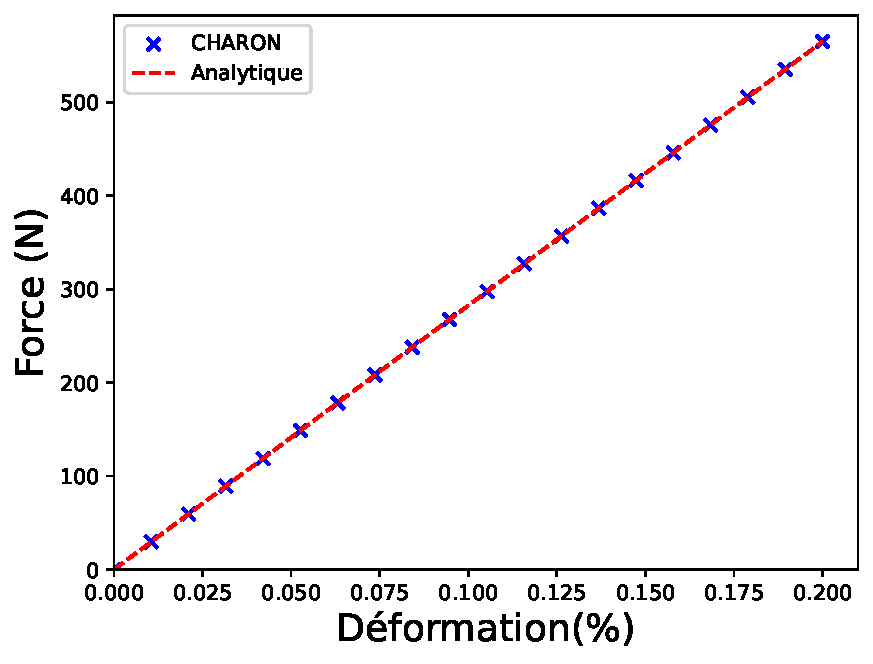
\includegraphics[width=\textwidth]{\path/1D_Traction_pseudo_2D}
\caption{Relation force-déformation en 2D-quasi 1D}
\label{fig:1D_Traction_pseudo_2D}
\end{subfigure}\hfill
\begin{subfigure}[b]{0.49\textwidth}
\centering 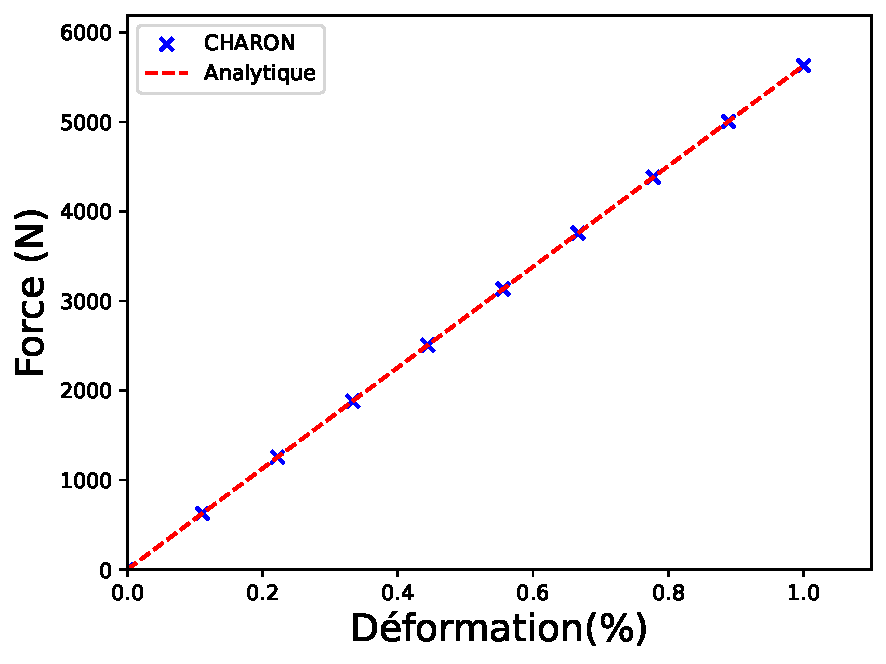
\includegraphics[width=\textwidth]{\path/1D_Traction_pseudo_3D}
\caption{Relation force-déformation en 1D pseudo-3D}
\label{fig:1D_Traction_pseudo_2D}
\end{subfigure}
\caption{Comparaison analytique numérique 1D via des modèles de dimensionnalités supérieures}
\label{fig:1D_Traction_pseudo_2_3D}
\end{figure}
\subsubsection{Compression cylindrique et sphérique avec le modèle 2D axi-symétrique}
Nous reprenons les modèles:
\begin{figure}[h!]
\begin{subfigure}[b]{0.35\textwidth}
\centering 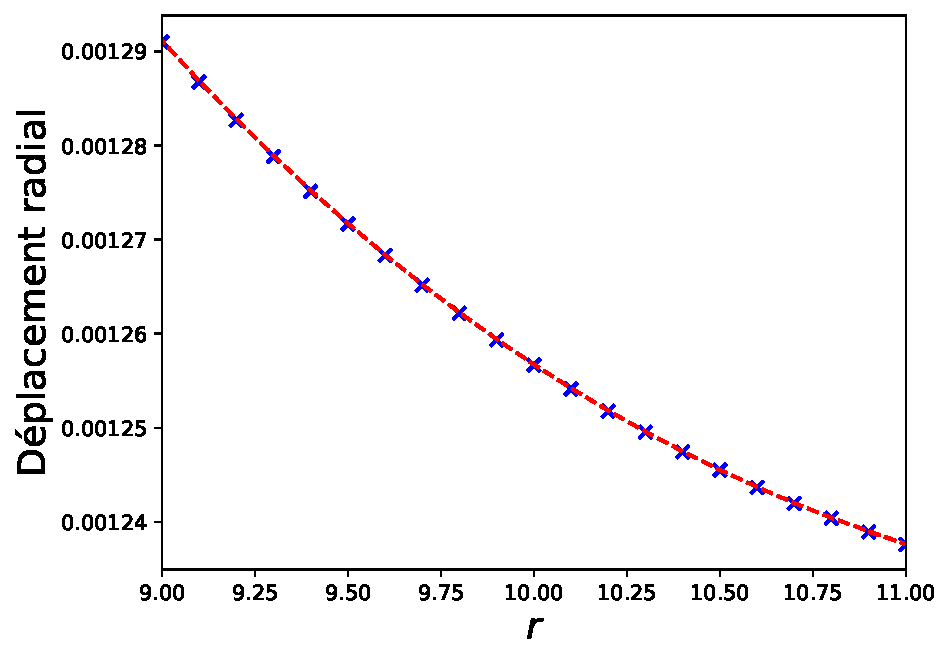
\includegraphics[width=\textwidth]{\path/1D_Cylindrique_compression_pseudo_2D}
\caption{Compression cylindrique 2D}
\label{fig:1D_Cylindrique_compression_pseudo_2D}
\end{subfigure}\hfill
\begin{subfigure}[b]{0.35\textwidth}
\centering 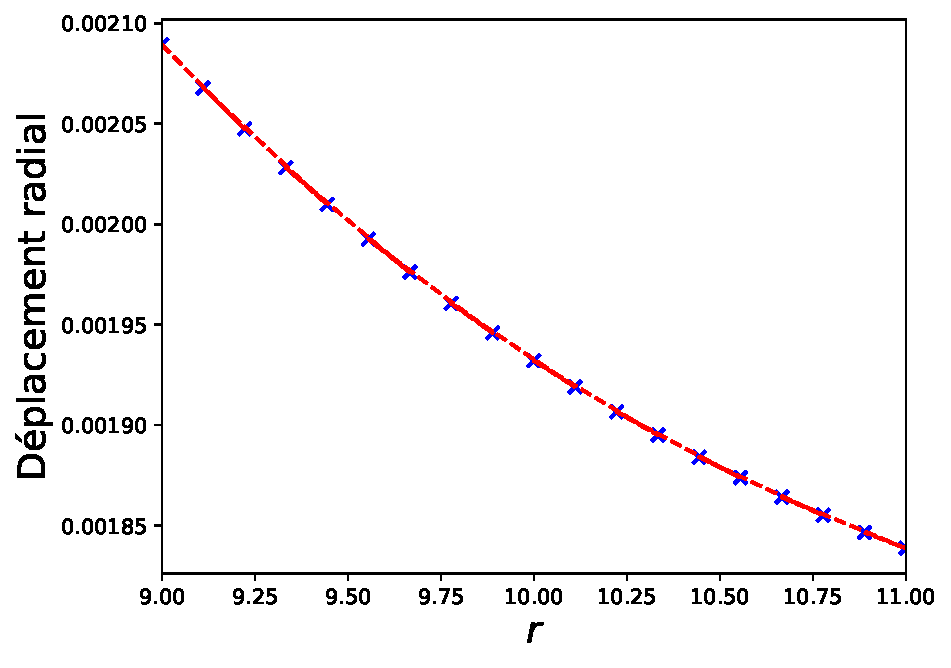
\includegraphics[width=\textwidth]{\path/1D_spherique_compression_pseudo_2D}
\caption{Compression sphérique 2D}
\label{fig:1D_spherique_compression_pseudo_2D}
\end{subfigure}
\begin{subfigure}[b]{0.28\textwidth}
\centering 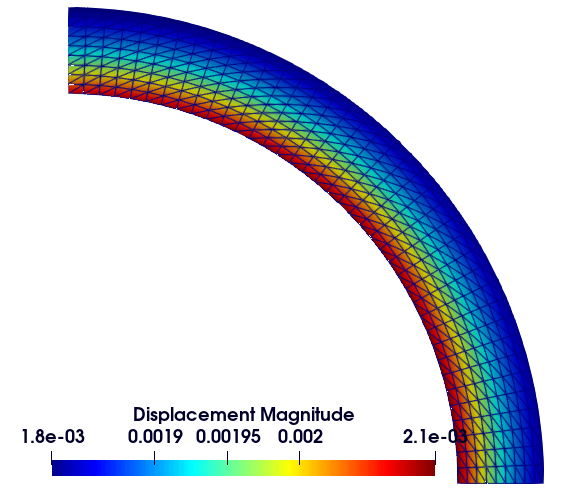
\includegraphics[width=\textwidth]{\path/deplacement_compression_axi}
\caption{Maillage sphérique 2D}
\label{fig:deplacement_compression_axi}
\end{subfigure}
\caption{Comparaison analytique numérique 1D}
\end{figure}
\subsection{Essais 2D}
\subsubsection{Traction uni-axiale en 2D plan}
Nous étudions la traction uni-axiale d'une plaque rectangulaire de dimensions $L=10\milli\metre$, $\ell = 0.5 \milli\metre$. Le matériau constitutif est un acier standard \eqref{eq:pte_acier_standard}. Nous annulons le déplacement $u_{x}$ sur le bord gauche et par symétrie, nous bloquons le déplacement vertical $u_{y}$ sur la partie inférieure. Le bord droit sera soumis soit à des conditions aux limites en déplacements soit en contraintes dans la direction $\ex$.

Sous ces conditions, la contrainte dans le plan est uni-axiale:
$$\SC = \sigma_{xx}\ex\otimes\ex+\sigma_{zz}\ez\otimes\ez=\sigma_{xx}\left(\ex\otimes\ex+\nu\ez\otimes\ez\right)$$
\paragraph{Condition aux limites en déplacement}
Nous imposons le déplacement $u_{x}$ sur le bord droit linéairement jusqu'à une valeur maximale $u_{x}^{\max}=0.1\milli\metre$. La déformation $\varepsilon_{xx}$ est uniforme:
$$\varepsilon_{xx}^{\max} = \dfrac{u_{x}^{\max}}{L} = 0.02$$
Tandis que la déformation transverse $\varepsilon_{yy}$ garantie l'annulation de la contrainte $\sigma_{yy}$:
$$\sigma_{yy}=0=\dfrac{E}{1+\nu}\left(\varepsilon_{yy}+\dfrac{\nu}{1-2\nu}\left(\varepsilon_{xx}+\varepsilon_{yy}\right)\right)\implique \varepsilon_{yy}=-\dfrac{\nu\varepsilon_{xx}}{1-\nu}$$
La relation $\sigma_{xx}=f(\varepsilon_{xx})$ est ensuite donnée par:
$$\sigma_{xx}=\dfrac{E}{1+\nu}\left(\varepsilon_{xx}+\dfrac{\nu}{1-2\nu}\varepsilon_{xxx}\left(1-\dfrac{\nu}{1-\nu}\right)\right)=\dfrac{E\varepsilon_{xx}}{1-\nu^{2}}$$
Nous représentons à la \figref{fig:traction_2D_plane_strain_dep} la courbe force-déformation pour la solution analytique et numérique.
\begin{figure}[h!]
\begin{subfigure}[b]{0.49\textwidth}
\centering 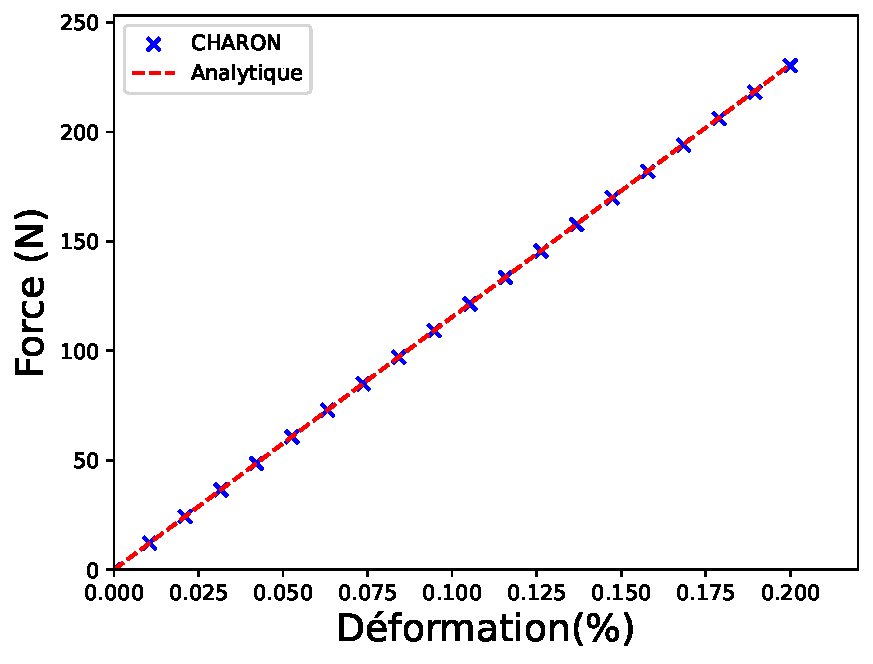
\includegraphics[width=0.8\textwidth]{\path/Traction_2D_Dirichlet}
\caption{Conditions limites en déplacements}
\label{fig:traction_2D_plane_strain_dep}
\end{subfigure}
\begin{subfigure}[b]{0.49\textwidth}
\centering 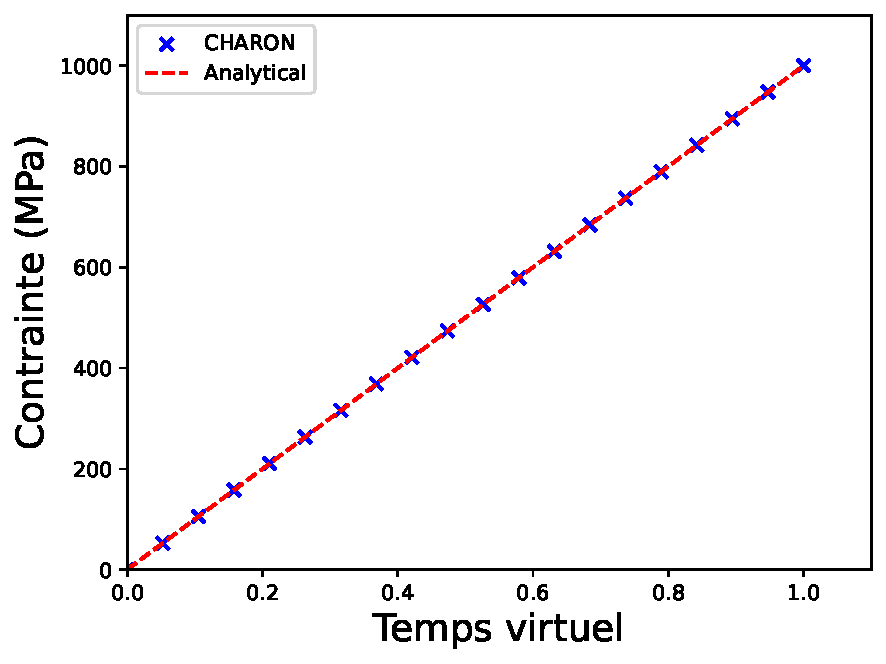
\includegraphics[width=0.8\textwidth]{\path/Traction_2D_Neumann}
\caption{Conditions limites en efforts}
\label{fig:traction_2D_plane_strain_F}
\end{subfigure}
\caption{Comparaison numérique-analytique de l'essai bi-dimensionnel de traction.}
\label{fig:traction_2D_plane_strain}
\end{figure}
\subsubsection{Compression cylindrique avec le modèle 2D axi-symétrique}
Nous utilisons ensuite le modèle axi-symétrique complet pour représenter un essai de compression cylindrique avec les bords supérieure et inférieure laissés libres. Le champ de déplacement est alors identique à celui donné à l'\eref{eq:analytical_Ur_1D_cyl} et comporte une composante verticale $u_{z}$ non nulle contrairement au modèle 1D cylindrique. Le champ de déplacement résultant est obtenu avec \eqref{eq:A_B_C_compression_cylindrique} en prenant $C=0$ et est représenté \figref{fig:2D_Cylindric_compression}.
\begin{figure}[h!]
\begin{subfigure}[b]{0.49\textwidth}
%\centering \includegraphics[width=0.8\textwidth]{\path/2D_Cylindric_compression}
\caption{Essai de compression d'un cylindre}
\label{fig:2D_Cylindric_compression}
\end{subfigure}
\begin{subfigure}[b]{0.49\textwidth}
%\centering \includegraphics[width=0.8\textwidth]{\path/2D_spherique_compression}
\caption{Essai de compression sphérique}
\end{subfigure}
\caption{Comparaison numérique-analytique de l'essai bi-dimensionnel de compression sous pression interne et extern.}
\label{fig:2D_Cylindric_compression}
\end{figure}
\subsubsection{Contrainte au bord d'une plaque trouée}
Nous étudions la traction uni-axiale d'une plaque percée par un trou circulaire de rayon $a$. La solution analytique constitue l'objet du chapitre 15 p.361 de \cite{forest2015mecanique}.
\begin{figure}[h!]
\centering 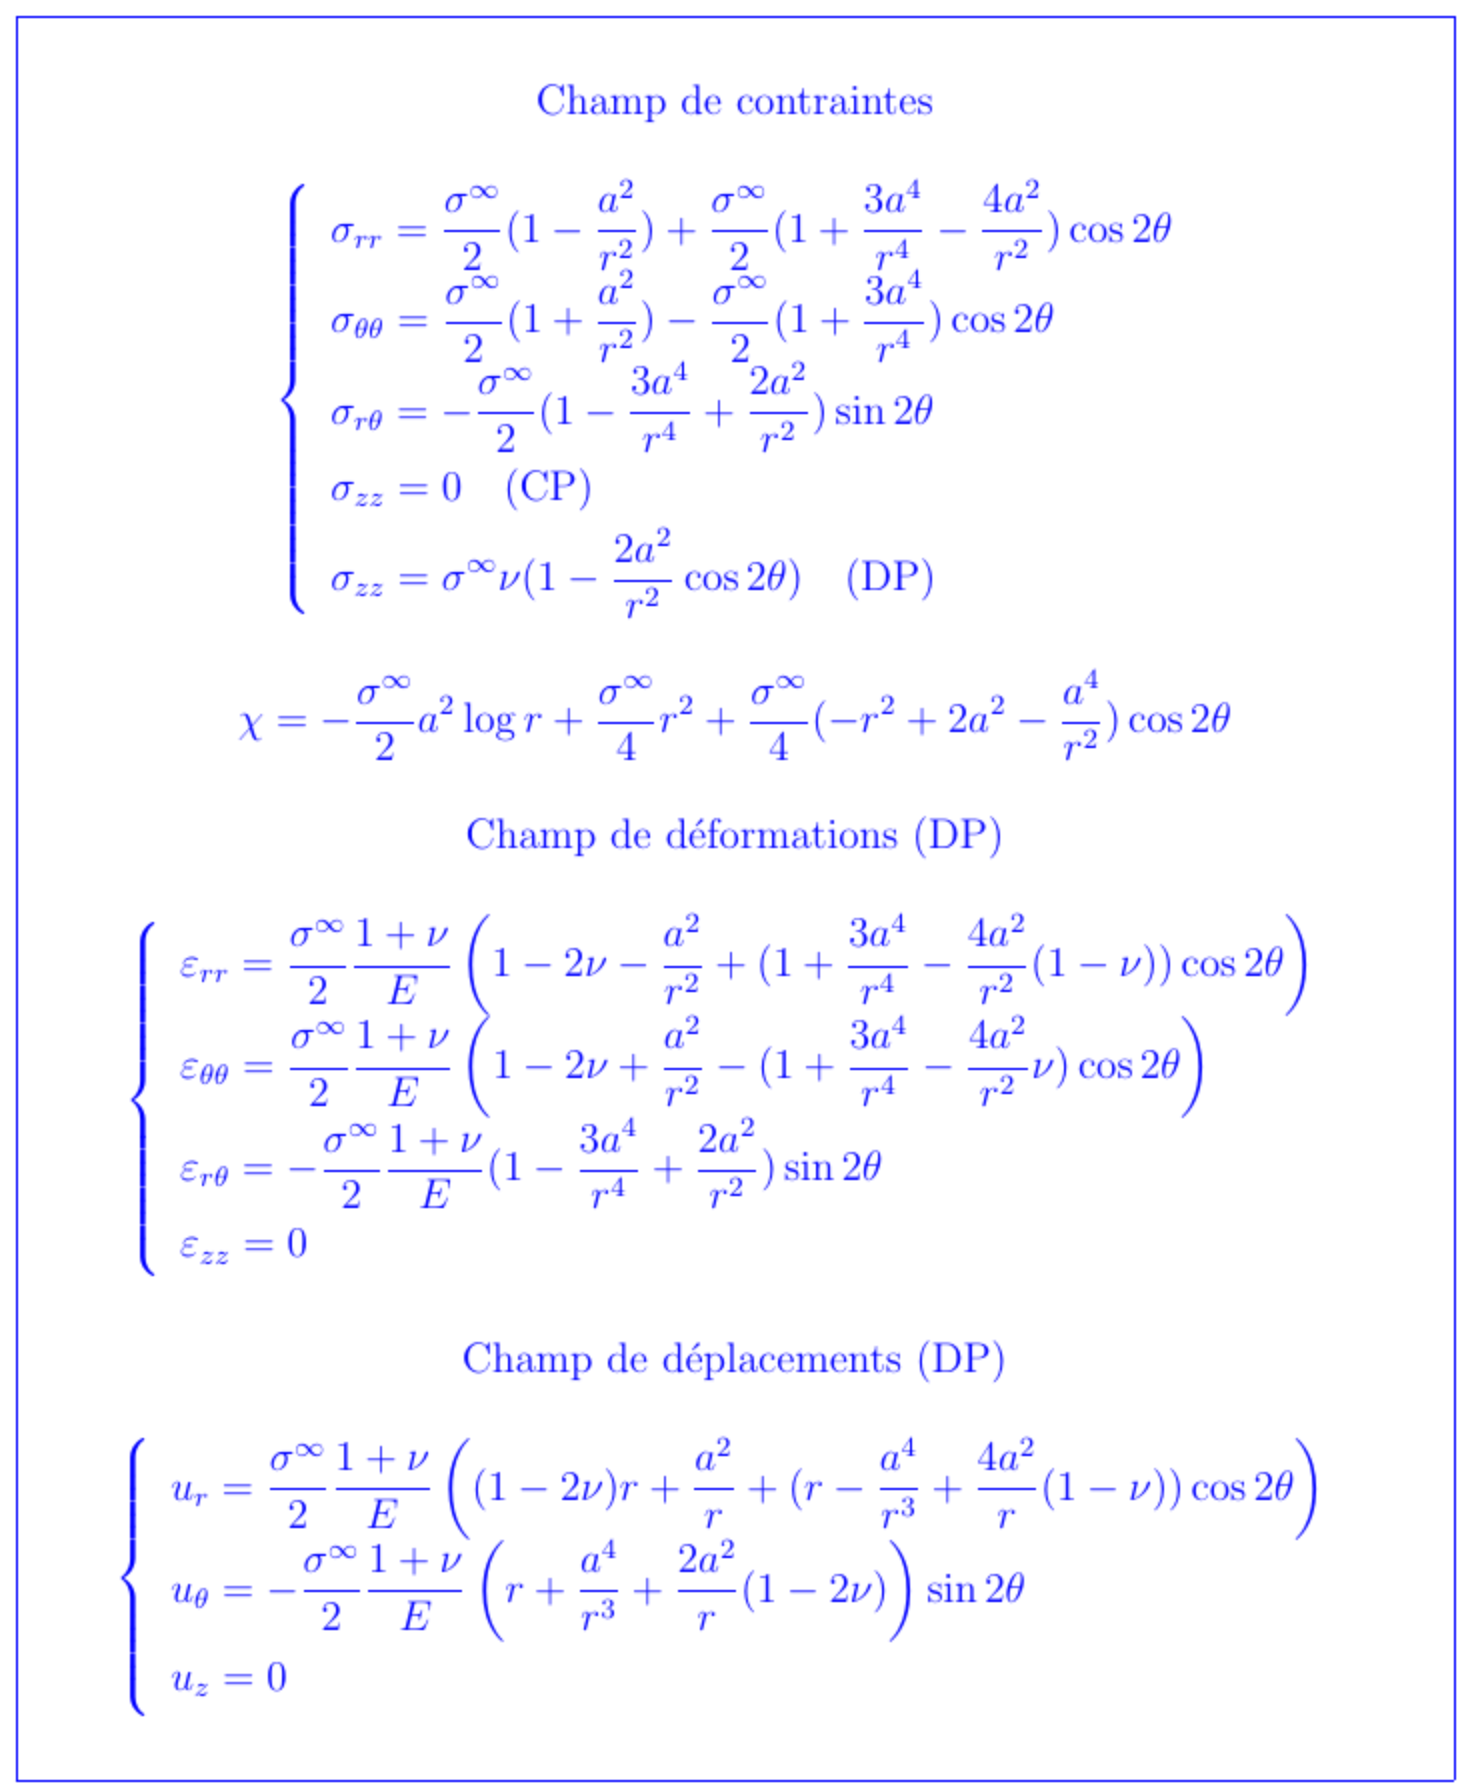
\includegraphics[width=0.8\textwidth]{\path/Plaque.trou_sol_Forest}
\end{figure}
Les contraintes sont analytiques, indépendamment du modèle de comportement mécanique retenu. En effet, les efforts au bord du trou sont complètement déterminés par l'équation d'équilibre. Nous pourrons donc comparer l'ensemble des modèles mécaniques et nous attendons à n'observer aucune différence en terme de contraintes. En revanche, seuls les déplacements correspondant à l'élasticité linéarisée de Hooke pourront être confrontés aux résultats.
\subsection{Traction uni-axiale en 3D}
Il s'agit ici de la \og vraie \fg{} expérience de traction. Le champ de contrainte est uniaxiale de la forme $\SC = \sig_{xx}\ex\otimes\ex$. La force de réaction associé au déplacement $\Dep$ induisant une déformation $\eps$, est donné par 
$$F = \sigma_{xx}S = E\varepsilon S$$
où $S$ désigne la section du solide. La comparaison analytique numérique est illustré à la \figref{fig:compa_analytique_num_elast_3D}
\begin{figure}[!h]
\centering 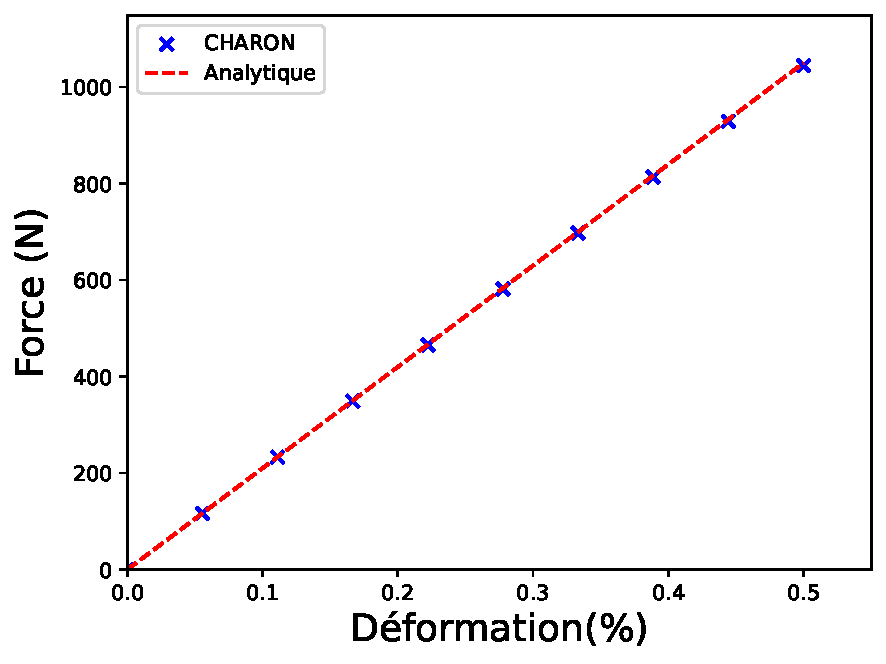
\includegraphics[width=0.7\textwidth]{\path/Traction_3D}
\caption{Évolution de l'effort de réaction en fonction de la déformation cas tridimensionnel}
\label{fig:compa_analytique_num_elast_3D}
\end{figure}
\FloatBarrier
\section{Elasto-Dynamique}
\subsection{Propagation d'une onde 1D}
\subsubsection{Propagation d'une onde 1D en cartésien}
Nous étudions la propagation d'un créneau de contrainte dans un matériau linéaire élastique isotrope. La géométrie est supposée unidimensionnelle cartésienne. La vitesse de propagation des ondes est classiquement donnée par:
$c=\sqrt{E/\rho}$ dans le cadre de l'hypothèse des petites perturbations. Si nous supposons que le signal appliqué est un créneau, de largeur $\ell=L/4$, sur l’extrémité gauche du solide de longueur $L$ à l'instant $t=0$, alors la contrainte est donnée à tout instant par:
$$\sigma = \sigma_{0}\times f(x-ct) \avec f(y)=\left\lbrace\begin{array}{ll}
1 & \si y\in[-\ell,0]\\
0 & \sinon
\end{array}\right.$$
La pseudo-viscosité ajoutée afin de stabiliser le calcul, amortie la solution du problème. Par conséquent, l’écart à la solution analytique peut devenir important si le pas spatial n'est pas suffisamment fin.
\paragraph{Comparaison analytique et numérique}
Nous observons à la \figref{fig:Elasticite_1D_cartesien} les solutions analytiques et numériques au problème de propagation. Les paramètres numériques utilisés sont consignés dans le \Tableref{Table:Parametres_nu_1D_carte}.
\begin{table}
\centering \begin{tabular}{lllll}\hline
$E(\mega\pascal)$  & $\nu$ & $L(\milli\metre)$ & $T_{fin}(\milli\second)$ & $\sigma_{0} (\mega\pascal)$\\
$210\times10^{3}$ & 0.3 & $50$ & $7.3\times 10^{-3}$ & $10^{4}$\\\hline
\end{tabular}
\caption{Paramètres numériques pour la propagation $1D$ cartésienne d'une onde de choc}
\label{Table:Parametres_nu_1D_carte}
\end{table}
Nous observons un excellent accord témoignant de la bonne implémentation du modèle $1D$ cartésien ainsi que du schéma temporel explicite. Pour les simulations \figref{fig:Elasticite_1D_cartesien}, les viscosités linéaire et quadratique sont diminuées à 0.02 et 0.1 respectivement.
\paragraph{Contraintes et solutions analytique}
\subparagraph{Modèlisation HPP} SI nous supposons que le comportement est donnée par l'hypothèse des petites perturbations alors:
$$\vdiv\SC = \rho\ddot{\Dep}\implique \dfrac{\partial}{\partial x}\left(-p+s_{xx}\right)=\rho\ddot{u_{x}}\implique (\kappa+2\mu)u_{,xx}=\rho u_{,tt}$$
Les solutions sont de la forme $\sigma_{xx} = f(x-ct)+g(x+ct)$ avec $c$ la célérité des ondes données par $c = \sqrt{\dfrac{\kappa+2\mu}{\rho}}=\sqrt{\dfrac{E}{\rho}}$.
\subsubsection{Propagation d'une onde 1D sphérique}
Pour un milieu élastique isotrope (module de Lamé $\lambda,\mu$, masse volumique $\rho$), la propagation d’ondes longitudinales (ondes P) en symétrie sphérique peut se modéliser par une seule fonction scalaire $u(r,t)$ représentant le déplacement radial (supposé uniquement radial, sans composante en $\theta$ ni en $\phi$).  

Sous ces hypothèses, l’équation de mouvement (équation d’onde) dans $\mathbb{R}^3$ se ramène à
$$\frac{1}{c_p^2}\,\frac{\partial^2 u}{\partial t^2}  -\frac{\partial^2 u}{\partial r^2}  -\frac{2}{r}\,\frac{\partial u}{\partial r} =0, \quad \text{où} \quad c_p =\sqrt{\frac{\lambda+2\mu}{\rho}}$$
Ici, $c_p$ est la vitesse des ondes P. Pour simplifier, on introduit la fonction
$$v(r,t) = r\;u(r,t)$$
En substituant $u = v/r$ dans l’équation ci-dessus, on montre (exercice classique) que $v$ satisfait une équation d’onde \emph{1D} standard :
$$\frac{1}{c_p^2}\,\frac{\partial^2 v}{\partial t^2} -\frac{\partial^2 v}{\partial r^2} =0$$
La solution générale de cette équation 1D (en variables $(r,t)$) s’écrit :
$$v(r,t) = f\Bigl(t - \tfrac{r}{c_p}\Bigr) + g\Bigl(t + \tfrac{r}{c_p}\Bigr)$$
d’où
$$u(r,t)=\frac{v(r,t)}{r}=\frac{1}{r}\,\Bigl[\,f\bigl(t - \tfrac{r}{c_p}\bigr)+ g\bigl(t + \tfrac{r}{c_p}\bigr)\Bigr]$$
\begin{itemize}
\item La partie $f(t - r/c_p)$ correspond à une onde \emph{sortante} (qui se propage vers $r \to +\infty$).  
\item La partie $g(t + r/c_p)$ correspond à une onde \emph{entrante} ou \emph{convergente} (qui se propage vers $r \to 0$).  
\end{itemize}
Supposons qu'à la frontière externe soit $r=R$, on impose un échelon de contrainte d'amplitude $A$. En régime linéaire, la composante radiale de la contrainte (pour un déplacement purement radial) vaut :
$$\sigma_{rr} = (\lambda + 2\mu)\,\frac{\partial u}{\partial r} + 2\lambda\,\frac{u}{r}$$
En réécrivant en termes de $v = ru$, on obtient :
$$\sigma_{rr}(r,t)  = (\lambda + 2\mu)\,\frac{1}{r}\,\frac{\partial v}{\partial r} + \frac{\lambda - 2\mu}{r^2}\,v$$
Appliquée à $r=R$, la condition devient :
$$\sigma_{rr}(R,t) = (\lambda + 2\mu)\,\frac{1}{R}\,\frac{\partial v}{\partial r}\Bigl|_{r=R} +
\frac{\lambda - 2\mu}{R^2}\,v(R,t) =
\text{(le créneau en fonction du temps).}$$
Or, $\partial v/\partial r$ à $r=R$ dépend de la dérivée de $f(t - R/c_p)$ et/ou $g(t + R/c_p)$.
\paragraph{Onde purement convergente.}
Si l’on \emph{ne veut} qu’une onde \emph{entrante} (c’est-à-dire qui se propage depuis $r=R$ vers le centre $r=0$), on prend classiquement
$$v(r,t) = g\!\Bigl(t + \tfrac{r}{c_p}\Bigr)$$
c’est-à-dire $f(\cdot) = 0$. On impose alors sur $r=R$ :
$$\sigma_{rr}(R,t)=(\lambda + 2\mu)\,\frac{1}{R}\,\frac{\d g}{\d\xi}\bigl(\xi\bigr)+
\frac{\lambda - 2\mu}{R^2}\;g\bigl(\xi\bigr)=S(t),\quad \xi = t + \frac{R}{c_p}$$
et $S(t)$ est la fonction $\sigma_{rr}(R,t)$ imposée.

C’est donc une équation différentielle linéaire (d’ordre 1) pour la fonction $g(\xi)$ en régime $t\ge 0$.
\paragraph{Comparaison analytique-numérique}
La comparaison des solutions analytique et numérique pour une coquille creuse constituée d'un acier standard est donnée à la \figref{fig:Compression_spherique_dynamique}. Les petits oscillations numériques pour la partie analytique est due à la résolution par  \texttt{scipy}.
\subsubsection{Propagation d'une onde 1D cylindrique}
Pour un milieu élastique isotrope (modules de Lamé $\lambda$, $\mu$, masse volumique $\rho$), la propagation d’ondes \emph{longitudinales} (\textit{ondes P}) en \emph{symétrie cylindrique} peut être décrite par un \emph{déplacement radial} $u(r,t)$ (pas de dépendance en $\theta$, et pas de composante axiale si l’on suppose une situation 2D dans la section transverse).  

L’équation d’onde, sous l’hypothèse de symétrie radiale, diffère légèrement de la version sphérique. En coordonnées cylindriques (2D), l’équation se ramène globalement à :
$$\frac{1}{c_p^2}\,\frac{\partial^2 u}{\partial t^2} \;-\;\frac{\partial^2 u}{\partial r^2} \;-\;\frac{1}{r}\,\frac{\partial u}{\partial r} \;=\;0, \quad \text{où} \quad c_p \;=\;\sqrt{\frac{\lambda + 2\mu}{\rho}}$$
(On remarque qu’en géométrie sphérique, il y avait un terme $-\tfrac{2}{r}\,\tfrac{\partial u}{\partial r}$, tandis qu’en cylindrique on a un seul facteur $-\tfrac{1}{r}\,\tfrac{\partial u}{\partial r}$.)

\paragraph{Onde libre.} 
Si on était en propagation \emph{libre} (pas de contrainte imposée au bord) et que l’on cherche une onde radiale de la forme 
$$u(r,t) \;=\;\frac{1}{\sqrt{r}}\;f\!\Bigl(t \pm \tfrac{r}{c_p}\Bigr)$$
cette dépendance en $1/\sqrt{r}$ apparaît naturellement en 2D. Ceci contraste avec le $1/r$ du cas \emph{3D sphérique} ou l’amplitude constante (en 1D plane).  
\paragraph{Formulation par fonction auxiliaire.} 
Si l’on impose \emph{une contrainte radiale} $\sigma_{rr}(R_{\text{out}},t)$ au rayon externe $r=R_{\text{out}}$, et que l’on s’intéresse à une \emph{onde entrante (convergente)}, on peut, par analogie au cas sphérique, poser :  
$$\underbrace{v(r,t)}_{\text{fonction auxiliaire}}
\;=\;
g\!\bigl(t + \tfrac{r}{c_p}\bigr)
\quad(\text{onde convergente pure}$$
puis relier $\sigma_{rr}(R_{\text{out}},t)$ à la dérivée de $v$ (ou directement à $g$) via la loi de Hooke en coordonnées cylindriques.  
\paragraph{Forme de \texorpdfstring{$\sigma_{rr}$}{sigma\_rr} en cylindrique.}
En régime linéaire, pour un déplacement purement radial en 2D cylindrique, on montre que :
$$\sigma_{rr} \;=\; (\lambda + 2\mu)\,\frac{\partial u}{\partial r} \;+\; \lambda\,\frac{u}{r} \;\;+\;\dots$$
(en fait, en 2D, la forme précise dépend des conventions, mais l’essentiel est que le coefficient devant $u/r$ n’est pas le même qu’en 3D).  

Si l’on exprime cela en fonction de $v(r,t) = \sqrt{r}\,u(r,t)$, on obtient une relation
$$\sigma_{rr}(r,t) \;=\; (\lambda + 2\mu)\,\underbrace{\Bigl[\cdots \frac{\partial v}{\partial r}\Bigr]}_{\text{termes en }1/\sqrt{r}} \;+\; \text{(autres termes)}\cdot \frac{v}{r}$$
Il s’avère qu’on récupère souvent un \emph{facteur} $\tfrac12$ qui apparaît devant l’un des termes (contrairement au cas 3D).  

\paragraph{Exemple d’équation différentielle.}
Au rayon $R_{\text{out}}$, la condition 
$$\sigma_{rr}\bigl(R_{\text{out}},t\bigr) \;=\; \sigma_{\text{ext}}(t)$$
mène à une \emph{équation différentielle} en $g(\xi)$, avec $\xi = t + \tfrac{R_{\text{out}}}{c_p}$, de la forme :
$$(\lambda + 2\mu)\,\frac{1}{R_{\text{out}}}\,g'(\xi) \;+\; \frac{\lambda - 2\mu}{2\,R_{\text{out}}^{2}}\,g(\xi) \;=\; \sigma_{\text{ext}}(t)$$
le facteur \(\tfrac12\) venant de la géométrie cylindrique. On peut résoudre cela par morceaux pour un \emph{créneau} $\sigma_{\text{ext}}(t)$, ou tout autre type de «\,pulse\,» imposé.
\paragraph{ Différences notables par rapport au cas sphérique}
\begin{itemize}
\item \textbf{Facteur 1/2} : en 2D cylindrique, la loi de Hooke et les termes de dérivée radiale font apparaître, lors du \emph{report} dans l’ODE au bord externe, un coefficient $\tfrac12$ sur le terme $g(\xi)$ (au lieu de $1$ en 3D). 
\item \textbf{Décroissance en } $\tfrac{1}{\sqrt{r}}$ : l’amplitude d’une onde «\,libre\,» (sans source ni contraintes) décroît comme $\tfrac{1}{\sqrt{r}}$ en cylindrique, contre $\tfrac{1}{r}$ en sphérique. Dans la résolution via une contrainte imposée, ce facteur se retrouve \emph{implicitement} dans la forme $u(r,t)$.
\end{itemize}
\begin{figure}
\begin{subfigure}[b]{0.32\textwidth}
\centering 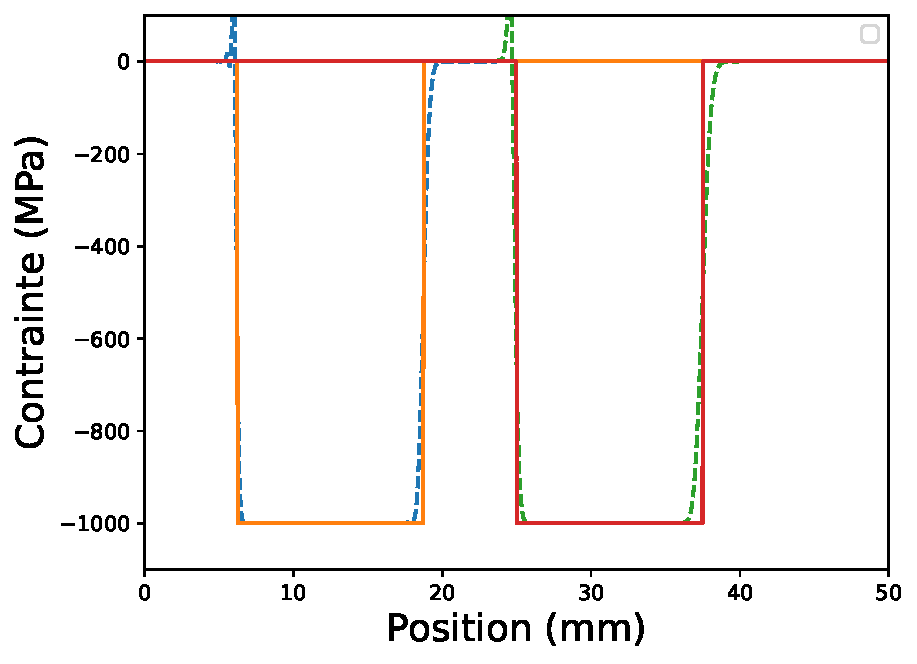
\includegraphics[width=\textwidth]{\path/Elasticite_1D_cartesien}
\caption{Contrainte à $t\in\{3.5,7\}\mu\second$.}
\label{fig:Elasticite_1D_cartesien}
\end{subfigure}
\begin{subfigure}[b]{0.32\textwidth}
\centering 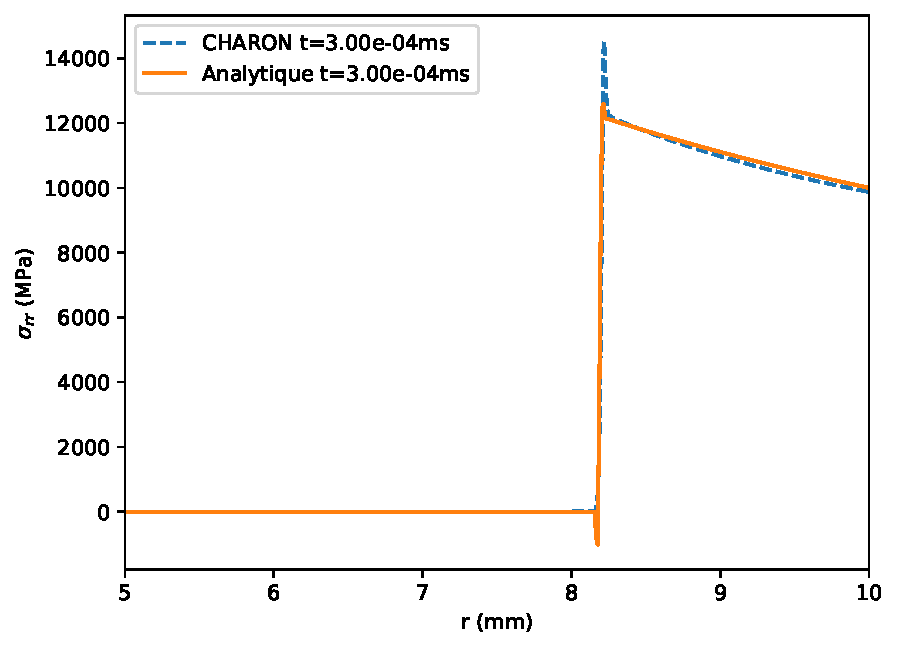
\includegraphics[width=\textwidth]{\path/Compression_spherique_dynamique}
\caption{Contrainte à $t=0.3\mu\second$}
\label{fig:Compression_spherique_dynamique}
\end{subfigure}
\begin{subfigure}[b]{0.32\textwidth}
\centering 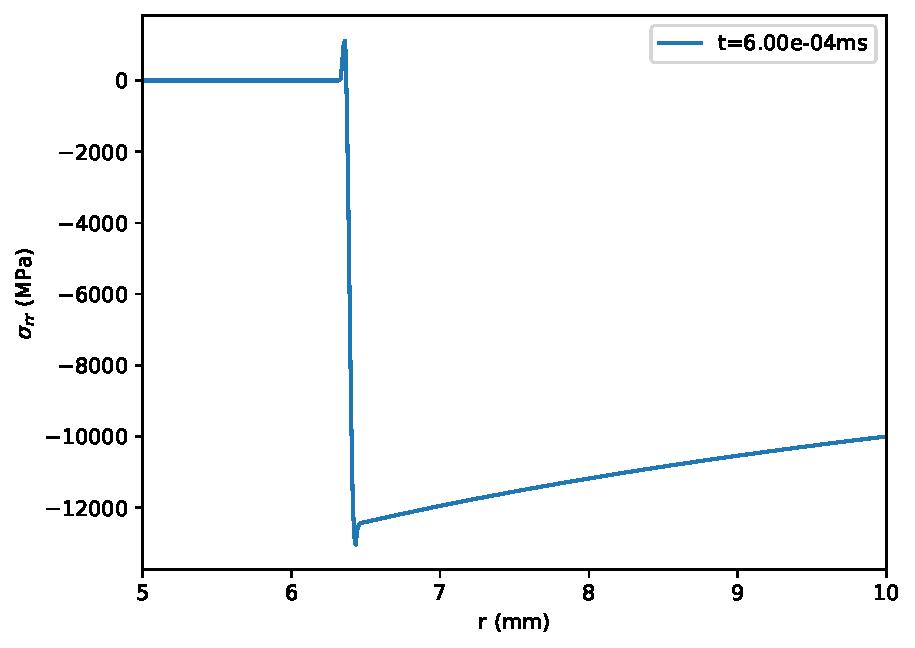
\includegraphics[width=\textwidth]{\path/Compression_cylindrique_dynamique}
\caption{Contrainte à $t=0.6\mu\second$}
\label{fig:Compression_cylindrique_dynamique}
\end{subfigure}
\caption{Comparaison analytique numérique d'une propagation d'onde.}
\label{fig:propagation_dynamique}
\end{figure}
\subsubsection{Tube à choc de Sod}
Le cas test du tube à choc de Sod \cite{sod1978survey} consiste à étudier l'évolution d'un cylindre initialement scindé en deux compartiments remplis du même gaz parfait ($\gamma=1.4$) mais dans deux états différents. La séparation entre les deux compartiments est enlevée à l'instant $t=0$. Dans le compartiment de gauche, le gaz est initialement au repos à $P_{0}=1$ et a une masse volumique $\rho=1$. Dans la partie droite, le gaz également au repos a une pression plus faible $P_{0}'=0.1$ et a une masse volumique réduite $\rho=0.125$. La mise en contact de ces deux milieux à l'instant initial induit la propagation d'une onde de compression dans le milieu peu dense et de détente dans le milieu dense. La solution analytique ainsi que le résultat fourni par CHARON à l'instant $t=0.2$ sont illustrés à la \figref{fig:comparaison_SOD}. Toute les grandeurs sont mentionnées ici sans unités.

La résolution numérique est issue du dépot git suivant:
\begin{center}
\url{https://gitlab.com/fantaz/simple_shock_tube_calculator}
\end{center}
\begin{figure}[h!]
\centering 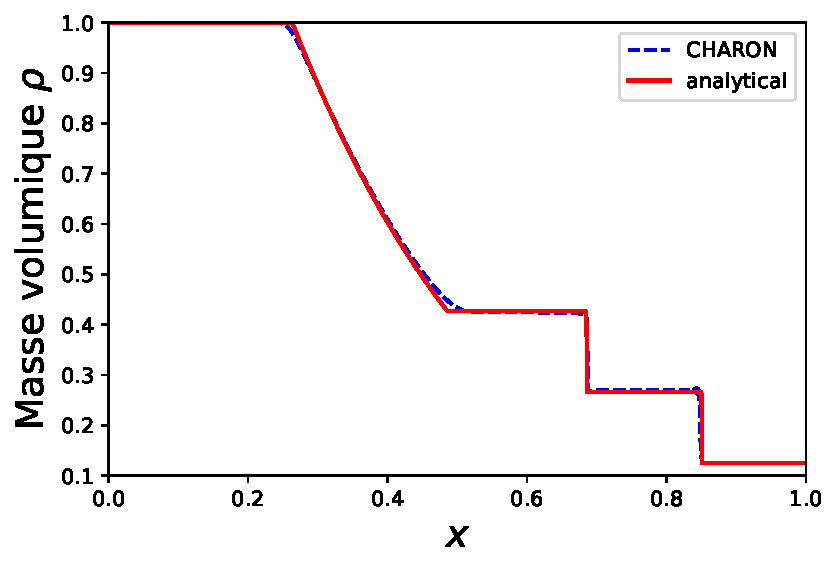
\includegraphics[width=0.8\textwidth]{\path/Tube_choc_Sod}
\caption{Comparaison numérique analytique de l'essai du tube à choc de Sod}
\label{fig:comparaison_SOD}
\end{figure}
\subsubsection{Réflexion transition d'un créneau sur une interface}
\paragraph{Équations fondamentales en élasticité linéaire 1D}
Dans un milieu élastique linéaire isotrope en 1D, le comportement est gouverné par trois équations fondamentales :
\begin{enumerate}
\item Équation de conservation de la quantité de mouvement :
$$\rho \frac{\partial^2 u}{\partial t^2} = \frac{\partial \sigma}{\partial x}$$
\item Loi de comportement en élasticité linéaire 1D :
$$\sigma = E^* \varepsilon = E^* \frac{\partial u}{\partial x}$$
où $E^*$ est le module élastique effectif en 1D donné par :
$$E^* = \frac{E(1-\nu)}{(1+\nu)(1-2\nu)}$$
Cette expression de $E^*$ provient de la réduction du tenseur d'élasticité 3D au cas 1D avec déformations latérales libres.
\item En combinant ces équations, on obtient l'équation d'onde :
$$\rho \frac{\partial^2 u}{\partial t^2} = E^* \frac{\partial^2 u}{\partial x^2}$$
\end{enumerate}
\paragraph{Vitesse de propagation et impédance acoustique}
La vitesse de propagation des ondes longitudinales est :
$$c = \sqrt{\frac{E^*}{\rho}} = \sqrt{\frac{E}{\rho} \frac{1-\nu}{(1+\nu)(1-2\nu)}}$$
L'impédance acoustique caractérise la résistance du milieu au passage de l'onde :
$$Z = \rho c = \sqrt{\rho E^*}$$
Pour une onde se propageant dans la direction positive, la solution générale prend la forme :
$$u(x,t) = f(t - \frac{x}{c}) + g(t + \frac{x}{c})$$
où $f$ représente l'onde progressive et $g$ l'onde rétrograde.
\paragraph{Interface entre deux milieux : conditions de continuité}
À l'interface entre deux milieux ($x = L$), deux conditions doivent être satisfaites :
\begin{enumerate}
\item Continuité du déplacement (pas de séparation) :
$$u_1(L,t) = u_2(L,t)$$
\item Continuité de la contrainte (équilibre des forces) :
$$\sigma_{\theta\theta}(L,t) = \sigma_{\varphi\varphi}(L,t)$$
\end{enumerate}
\paragraph{Coefficients de réflexion et transmission}
Pour une onde incidente arrivant sur l'interface, on peut écrire :
$$u_{tot}(x,t) = \begin{cases}
u_i(x,t) + u_r(x,t) & \text{pour } x < L \\
u_t(x,t) & \text{pour } x > L
\end{cases}$$
En appliquant les conditions de continuité et en utilisant la relation $u_t = \frac{\sigma}{Z}$ pour les ondes progressives, on obtient :
$$R = \frac{Z_2 - Z_1}{Z_1 + Z_2}, \quad T = \frac{2Z_2}{Z_1 + Z_2}$$
Ces coefficients ont des propriétés importantes :
\begin{itemize}
\item $R + T = 1$ (conservation de l'énergie)
\item $-1 \leq R \leq 1$ (limitation physique de l'amplitude réfléchie)
\item Le signe de $R$ dépend du contraste d'impédance :
\begin{itemize}
\item $R > 0$ si $Z_2 > Z_1$ (réflexion en phase)
\item $R < 0$ si $Z_2 < Z_1$ (réflexion en opposition de phase)
\end{itemize}
\end{itemize}
\paragraph{Solution pour un pulse de contrainte}
Pour un pulse de contrainte rectangulaire :
$$\sigma_i(t) = \begin{cases}
\sigma_0 & \text{pour } 0 \leq t < T_{pulse} \\
0 & \text{sinon}
\end{cases}$$
Les déplacements sont obtenus par intégration temporelle :
\begin{enumerate}
\item Onde incidente :
$$u_i(x,t) = \frac{1}{Z_1}\int_0^{t-x/c_1} \sigma_i(\tau) d\tau = \begin{cases}
\frac{\sigma_0}{Z_1}(t-x/c_1) & \text{pour } 0 \leq t-x/c_1 < T_{pulse} \\
\frac{\sigma_0}{Z_1}T_{pulse} & \text{pour } t-x/c_1 \geq T_{pulse}
\end{cases}$$
\item Onde réfléchie :
$$u_r(x,t) = \frac{R}{Z_1}\int_0^{t-(2L-x)/c_1} \sigma_i(\tau) d\tau$$
\item Onde transmise :
$$u_t(x,t) = \frac{T}{Z_2}\int_0^{t-(L/c_1+(x-L)/c_2)} \sigma_i(\tau) d\tau$$
\end{enumerate}
\paragraph{Calcul des contraintes à partir des déplacements}
Les contraintes sont obtenues par dérivation spatiale :
$$\sigma = \rho c^2 \frac{\partial u}{\partial x} = E^* \frac{\partial u}{\partial x}$$
Pour le pulse rectangulaire, on obtient :
\begin{enumerate}
\item Onde incidente :
$$\sigma_i(x,t) = \begin{cases}
\sigma_0 & \text{pour } 0 \leq t-x/c_1 < T_{pulse} \\
0 & \text{sinon}
\end{cases}$$
\item Onde réfléchie :
$$\sigma_r(x,t) = \begin{cases}
R\sigma_0 & \text{pour } 0 \leq t-(2L-x)/c_1 < T_{pulse} \\
0 & \text{sinon}
\end{cases}$$
\item Onde transmise :
$$\sigma_t(x,t) = \begin{cases}
T\sigma_0 & \text{pour } 0 \leq t-(L/c_1+(x-L)/c_2) < T_{pulse} \\
0 & \text{sinon}
\end{cases}$$
\end{enumerate}
\paragraph{Application au cas acier/aluminium}
Pour l'interface acier/aluminium :
\begin{itemize}
\item $Z_{\text{acier}} > Z_{\text{alu}}$ car $\rho_{\text{acier}}c_{\text{acier}} > \rho_{\text{alu}}c_{\text{alu}}$
\item Donc $R < 0$ : l'onde réfléchie est en opposition de phase avec l'onde incidente
\item Pour une compression incidente ($\sigma_0 < 0$), l'onde réfléchie est en tension ($\sigma_r > 0$)
\item L'onde transmise garde le signe de l'onde incidente mais avec une amplitude réduite
\end{itemize}
La comparaison entre la solution analytique et numérique est donnée à la \figref{fig:Reflexion_bimat}
\begin{figure}[h!]
\centering 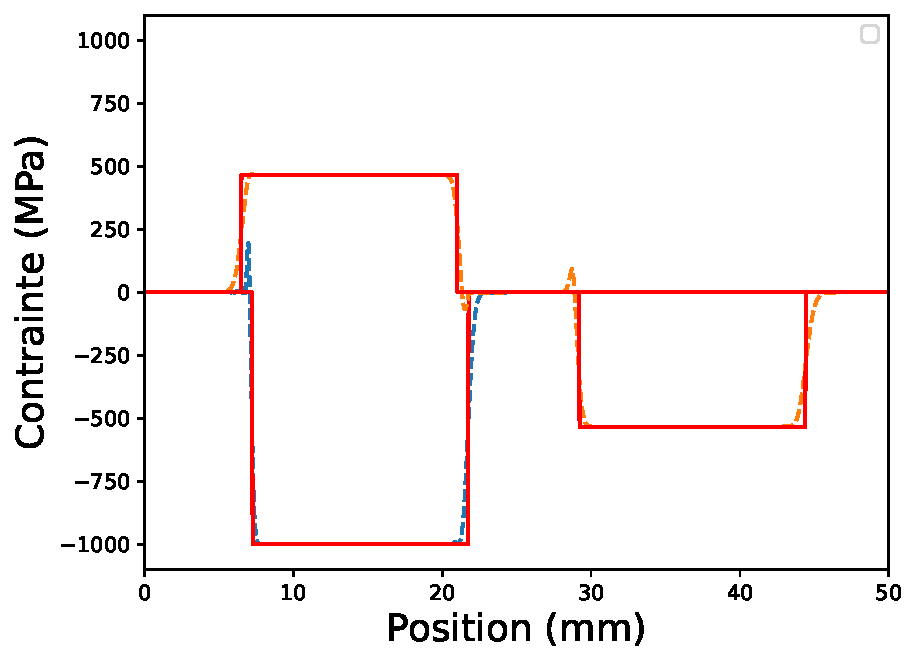
\includegraphics[width=0.5\textwidth]{\path/Reflexion_bimat}
\caption{Réflexion d'un créneau de contrainte à l'interface entre deux matériaux.}
\label{fig:Reflexion_bimat}
\end{figure}
\subsection{Essai 1D pseudo 2D}
A nouveau l'enjeu de cette section est de vérifier le bon comportement de nos modèles bi ou tri-dimensionnel en reistreignant les bords de manière a se ramener à un essai 1D
\subsubsection{Onde pseudo-1D cartésienne}
Nous reprenons comme précédemment le cas d'étude d'une propagation d'onde dans un barreau, cette fois représenté avec un modèle 2D plan. Afin de simuler correctement un champ de déplacement de la forme $\Dep=u_{x}(x)\ex$, nous devons bloquer tout les déplacements latéraux sans quoi, par effet poisson, le barreau se contractera et se dilatera dans la direction orthogonale au passage de l'onde. Nous relevons la contrainte le long de la barre et vérifions comme précédemment la bonne propagation du créneau. 
\subsubsection{Onde 1D avec le modèle axisymétrique}
\section{Diffusion thermique}
Nous prenons pour référence le \og HandBook of Heat Transfer \fg{} Rohsenow et Hartnett dans lequel nous pouvons trouver des solutions partie 3.26 correspondant aux pages 154 et suivantes.
\FloatBarrier
\subsection{Diffusion thermique d'un créneau}
Nous étudions la diffusion pure (hydro-dynamique désactivée) d'un créneau de température.
\subsection{Diffusion $1D$}
\paragraph{Position du problème}
Le modèle retenu est unidimensionnel cartésien. Le champ de température initial est donnée par:
$$T=\left\lbrace\begin{array}{ll}
T_{c} &\si [x_{\min},x_{\max}]\\
T_{f} & \sinon
\end{array}\right.$$
Le barreau, d'une longueur $L$, a son origine spatiale fixée arbitrairement sur le bord gauche. $x_{\min}$ et $x_{\max}$ sont choisis loin des extrémités de façon à éliminer les effets de bords. 
\paragraph{Solution analytique}
Alors la solution analytique est donnée par:
$$T(x,t)=\dfrac{T_{c}-T_{f}}{2}\left(erf\left(\dfrac{x+x_{\max}}{D}\right)+erf\left(\dfrac{x+x_{\min}}{D}\right)\right)+T_{f} \avec D=\sqrt{\dfrac{4\lambda t}{\rho C_{v}}}$$
et où $erf$ désigne la fonction erreur:
$$erf(x)=\dfrac{2}{\sqrt{\pi}}\int_{0}^{x} e^{-t^{2}}\dt$$
\ToDo{Source}
\paragraph{Comparaison numérique} Les paramètres numériques retenus sont les suivants:
\begin{table}[h!]
\centering \begin{tabular}{llllll}\hline
Conductivité & Masse volumique & Capacité thermique & Longueur & Taille créneau  & Temps final\\
$\lambda=240$ & $\rho_{0}=2785$ & $C_{v}=$ & $L=205$ & $\ell=1$ & $T_{fin}=1\times 10^{-6}$\\\hline
\end{tabular}
\end{table}
Nous obtenons alors l'évolution du champ de température suivante (voir \figref{fig:diffusion_1D}):
\begin{figure}[h!]
\centering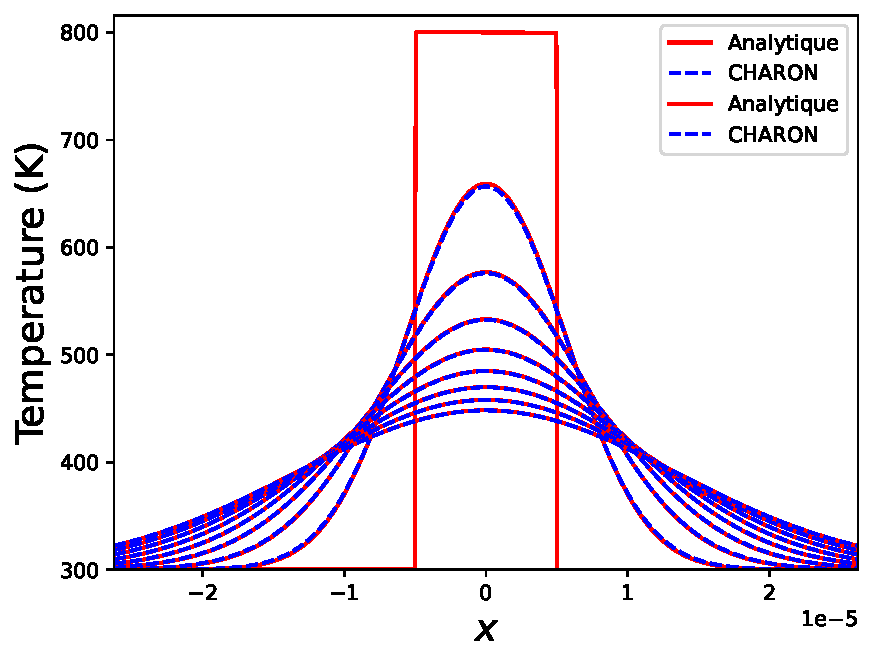
\includegraphics[width=0.65\textwidth]{\path/diffusion_1D}
\caption{Comparaison analytique-numérique concernant la diffusion thermique en 1D cartésien pour $t\in[0,0.125,0.25,0.375,0.5,0.675,0.75,0.875,1]\mu\second$}
\label{fig:diffusion_1D}
\end{figure}

L'accord est quasiment parfait et témoigne du bon fonctionnement de notre schéma en cartésien unidimensionnel.
\FloatBarrier
\section{Plasticité}
\subsection{Expansion élasto-plastique d'une sphère}
La forme intégrale de la solution analytique pour le problème d'une sphère creuse élasto-plastique soumise à des charges uniformes est présentée. Cette équation intégrale est résolue par un schéma d'intégration numérique.
\subsubsection{Position du problème}
\begin{figure}[h!]
\centering 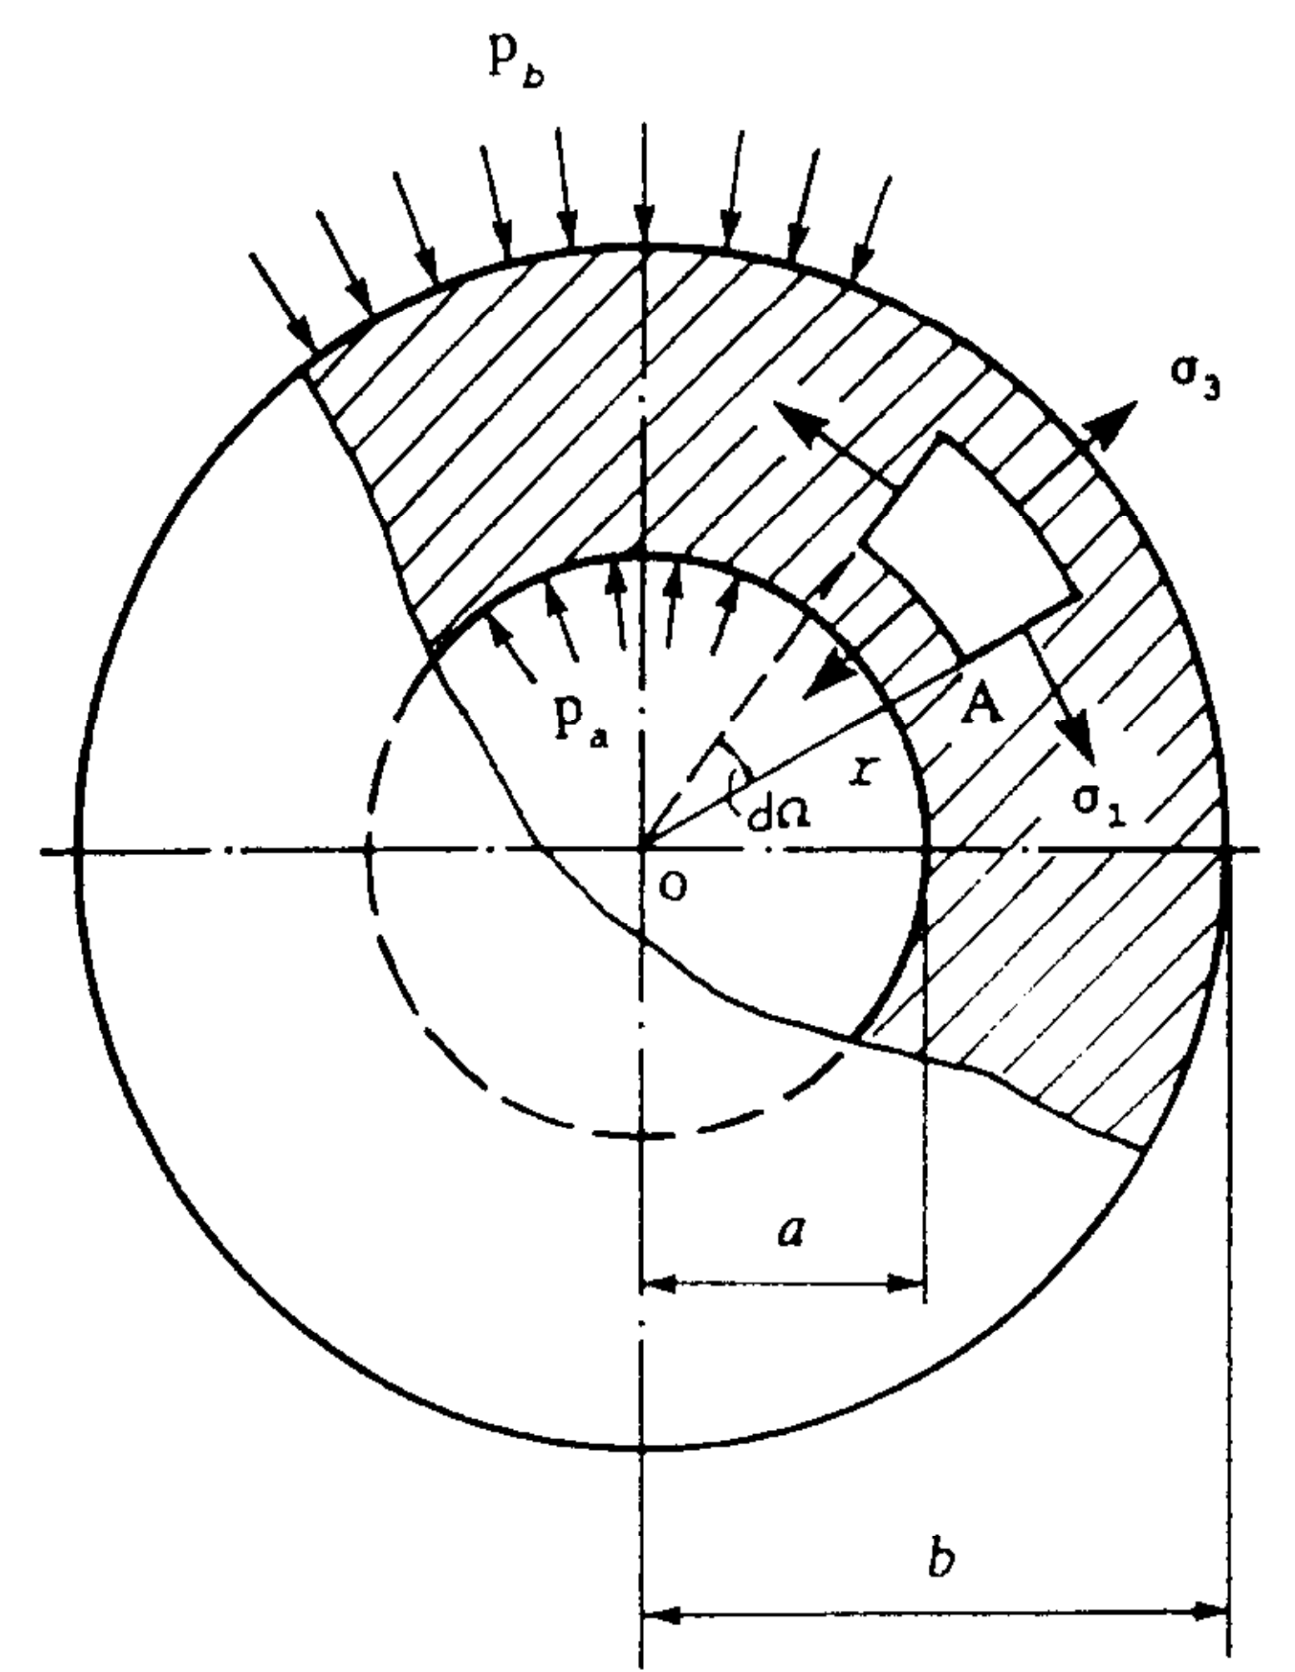
\includegraphics[width=0.5\textwidth]{\path/sphere_elasto_plastique}
\caption{Représentation schématique d'une boule creuse soumise à un effort de pression externe et interne}
\label{fig:sphere_elasto_plastique}
\end{figure}
La \figref{fig:sphere_elasto_plastique} est une représentation schématique d'une sphère creuse de rayon interne $a$ et de rayon externe $b$. La sphère est soumise à une pression uniforme interne $p_{int}$ et une pression uniforme externe $p_{ext}$. En raison de la symétrie de la géométrie et du chargement, les axes principaux pour les contraintes et les déformations se situent dans la direction radiale $r$ (notée par l'indice 3 dans la figure) et les deux directions orthogonales perpendiculaires à $r$ (celles-ci sont notées par les indices 1 et 2). En adoptant les notations d'indices précédentes, la contrainte et la déformation radiales peuvent être représentées par $\sigma_{rr}$ et $\varepsilon_{rr}$, et les contraintes et déformations tangentielles par $\sigma_{\theta\theta} = \sigma_{\varphi\varphi}$ et $\varepsilon_{\theta\theta} = \varepsilon_{\varphi\varphi}$, respectivement.
\subsubsection{Solution élasto-plastique}
Au point $A$, le déplacement radial est $u_{r}(r)$ et les déplacements tangentiels sont nuls (en raison de la symétrie). Les relations déformation-déplacement sont :
\begin{equation}
\varepsilon_{rr} = \frac{\d u_{r}}{\dr}, \quad \varepsilon_{\theta\theta} = \varepsilon_{\varphi\varphi} = \frac{u_{r}}{r}
\label{eq:Vaziri_defi_defo_sph}
\end{equation}
La déformation volumétrique dans l'hypothèse des petites perturbations est :
\begin{equation}
\tr\DefoHPP = \varepsilon_{\theta\theta} + \varepsilon_{\varphi\varphi} + \varepsilon_{rr} = 2\varepsilon_{\theta\theta} + \varepsilon_{rr}
\label{eq:Vaziri_defi_defo_vol}
\end{equation}
Et nous définissons la déformation effective par :
\begin{equation}
\bar{\varepsilon} = \frac{2}{3}|\varepsilon_{\theta\theta} - \varepsilon_{rr}| = \frac{2}{3}\Psi(\varepsilon_{\theta\theta} - \varepsilon_{rr}) \times (\varepsilon_{\theta\theta} - \varepsilon_{rr}) \avec \Psi:x\mapsto\sign(x)= \begin{cases}
1.0 & \text{quand } x \geq 0\\
-1.0 & \text{quand } x < 0
\end{cases}
\label{eq:Vaziri_defi_defo_eff}
\end{equation}
Nous montrerons plus tard  (voir \eqref{eq:forme_alternative_Psi}) que le signe de $\varepsilon_{\theta\theta} - \varepsilon_{rr}$ est plus simplement donné par le signe de $p_{i}-p_{e}$. Dans la suite, nous noterons plus sobrement $\Psi$ pour désigner $\pm 1$ en se rappelant que la valeur de $\Psi$ est donné par le signe de la différence $\varepsilon_{\theta\theta} - \varepsilon_{rr}$.

Nous définissons alors la contrainte hydrostatique et effective respectivement par :
\begin{equation}
\sigma = \frac{1}{3}(\sigma_{\theta\theta} + \sigma_{\varphi\varphi} + \sigma_{rr}) = \frac{1}{3}(2\sigma_{\theta\theta} + \sigma_{rr}); \qquad 
\bar{\sigma} = \Psi(\sigma_{\theta\theta} - \sigma_{rr})
\label{eq:Vaziri_defi_sig_eff}
\end{equation}
En supposant des conditions de chargement uniforme, les relations de comportement pour un matériau élasto-plastique peuvent être représentées par :
\begin{align}\label{eq:Vaziri_loi_compo_sig}
\sigma &= \BulkModulus\tr\DefoHPP && \text{Loi élastique linéaire en volume}\\\label{eq:Vaziri_loi_compo_sig_eff}
\bar{\sigma} &= \phi(\bar{\varepsilon})&& \text{Loi élasto-plastique générique en cisaillement}
\end{align}
où $\BulkModulus$ est le module de compressibilité et $\phi$ est la fonction de résistance en contrainte effective, qui peut être déterminée en effectuant un essai de traction uniaxiale.

La condition d'équilibre peut maintenant être obtenue en égalant à zéro les composantes de contrainte dans la direction radiale, soit :
\begin{equation}
\frac{\d\sigma_{rr}}{\dr} + \frac{2}{r}(\sigma_{\theta\theta} - \sigma_{rr}) = 0
\label{eq:Vaziri_condition_equilibre}
\end{equation}
Les conditions aux limites pertinentes pour le problème sont :
\begin{align}\label{eq:Vaziri_BCs_int}
\sigma_{rr} = -p_{int} \quad \text{quand } r = a\\\label{eq:Vaziri_BCs_ext}
\sigma_{rr} = -p_{ext} \quad \text{quand } r = b
\end{align}
Les équations \eqref{eq:Vaziri_defi_defo_sph}, \eqref{eq:Vaziri_loi_compo_sig}, \eqref{eq:Vaziri_loi_compo_sig_eff} et \eqref{eq:Vaziri_condition_equilibre} sont les équations gouvernantes représentant la compatibilité, l'équilibre et les conditions de contrainte-déformation pour le problème considéré.

En utilisant l'équation \eqref{eq:Vaziri_defi_sig_eff} et en réarrangeant, \eqref{eq:Vaziri_condition_equilibre} peut être exprimée comme :
\begin{equation}
\left(\frac{\d\bar{\sigma}}{\dr} + \frac{2}{r}\bar{\sigma}\right) - \Psi\frac{\d\sigma_{\theta\theta}}{\dr} = 0
\label{eq:Vaziri_condition_equilibre_equiv}
\end{equation}
En utilisant les relations montrées dans les équations \eqref{eq:Vaziri_defi_defo_vol}-\eqref{eq:Vaziri_defi_sig_eff}, \eqref{eq:Vaziri_loi_compo_sig} peut s'écrire :
\begin{equation}
\sigma_{\theta\theta} = \frac{1}{3}\Psi\bar{\sigma} - \frac{1}{3}\Psi \BulkModulus\bar{\varepsilon} + \BulkModulus\varepsilon_{\theta\theta}
\label{eq:Vaziri_loi_compo_sig_tt}
\end{equation}
En utilisant l'équation \eqref{eq:Vaziri_loi_compo_sig_tt} et notant les relations montrées dans les équations \eqref{eq:Vaziri_defi_defo_sph} et \eqref{eq:Vaziri_defi_defo_eff} :
$$\frac{\d\varepsilon_{\theta\theta}}{\dr} = \frac{1}{r}\left(\frac{\d w}{\dr} - \frac{w}{r}\right) = \frac{1}{r}(\varepsilon_{rr} - \varepsilon_{\theta\theta}) = \Psi\frac{\bar{\varepsilon}}{r}$$
alors l'équation \eqref{eq:Vaziri_condition_equilibre_equiv} peut s'écrire sous la forme suivante :
$$\frac{2}{3}\frac{\d\bar{\sigma}}{\dr} + \frac{2}{r}\bar{\sigma} + \frac{3}{2}\BulkModulus\frac{\d\bar{\varepsilon}}{\dr} + \frac{9}{2}\BulkModulus\frac{\bar{\varepsilon}}{r} = 0$$
ou après réarrangement :
$$\frac{\d}{\dr}\left(\bar{\sigma} + \frac{9}{4}\BulkModulus\bar{\varepsilon}\right) + \frac{3}{r}\left(\bar{\sigma} + \frac{9}{4}\BulkModulus\bar{\varepsilon}\right) = 0$$
Cette équation peut être facilement résolue, la solution étant :
\begin{equation}
\bar{\sigma} + \frac{9}{4}\BulkModulus\bar{\varepsilon} = \frac{C}{r^3}
\label{eq:Vaziri_sol_sig_eff}
\end{equation}
où $C$ est une constante.

À partir de l'équation \eqref{eq:Vaziri_condition_equilibre}, nous avons :
\begin{equation}
\sigma_{rr} = 2\int_a^r\frac{\Psi}{r}\bar{\sigma}\dr + C'
\label{eq:Vaziri_sol_sig_rr}
\end{equation}
Basé sur la condition aux limites montrée par l'équation \eqref{eq:Vaziri_BCs_int}, $C' = -p_{int}$.

Les équations \eqref{eq:Vaziri_sol_sig_rr}, \eqref{eq:Vaziri_sol_sig_eff} et \eqref{eq:Vaziri_loi_compo_sig_eff} ainsi que la condition aux limites donnée par l'équation \eqref{eq:Vaziri_BCs_ext} forment maintenant les équations de base pour le problème. En substituant l'équation \eqref{eq:Vaziri_loi_compo_sig_eff} dans \eqref{eq:Vaziri_sol_sig_eff} et \eqref{eq:Vaziri_sol_sig_rr}, on obtient :
\begin{align}\label{eq:system_analyitique_fin_1}
\phi(\bar{\varepsilon}) + \frac{9}{4}\BulkModulus\bar{\varepsilon} = \frac{C}{r^3}\\\label{eq:system_analyitique_fin_2}
\sigma_{rr} = 2\int_a^r\frac{\Psi}{r}\phi(\bar{\varepsilon})\dr - p_{int}\\\label{eq:system_analyitique_fin_3}
\sigma_{rr}(b) = -p_{ext}
\end{align}
En posant $r = b$ dans l'équation \eqref{eq:system_analyitique_fin_2}, on peut montrer que :
$$p_{int} - p_{ext} = 2\int_a^b\frac{\Psi}{r}\phi(\bar{\varepsilon})\dr$$
Puisque $r$ et $\phi(\bar{\varepsilon})$ sont des quantités positives, $\Psi$ doit être du même signe que $(p_{int} - p_{ext})$. On peut donc établir que :
\begin{equation}
\Psi = \text{sign}(p_{int} - p_{ext}) = \begin{cases}
1.0 & \text{quand } (p_{int} - p_{ext}) \geq 0\\
-1.0 & \text{quand } (p_{int} - p_{ext}) < 0
\end{cases}
\label{eq:forme_alternative_Psi}
\end{equation}
Il peut être noté que puisqu'il y a maintenant deux équations (équations \eqref{eq:system_analyitique_fin_1} et \eqref{eq:system_analyitique_fin_2}) pour deux variables ($\bar{\varepsilon}$ et $\sigma_{rr}$) et qu'il y a une équation de condition aux limites (équation \eqref{eq:system_analyitique_fin_3}) pour une constante [$C$ dans l'équation \eqref{eq:system_analyitique_fin_1}], alors la solution du problème est uniquement déterminée.\\

L'intégration numérique est utilisée pour résoudre l'équation \eqref{eq:system_analyitique_fin_2} ; la détermination de $\bar{\varepsilon}$ et $\sigma_{rr}$ dépend donc du nombre de points d'intégration adoptés. La technique de solution proposée est la suivante.

En introduisant un paramètre de déviation, $\Delta$, défini par :
\begin{equation}
\Delta = p_{ext} + \sigma_{rr}(b)
\label{eq:residu_p_ext_hollow}
\end{equation}
le problème peut être transformé en la recherche d'une valeur correcte de $C$ et la résolution des équations \eqref{eq:system_analyitique_fin_1} et \eqref{eq:system_analyitique_fin_2} de telle sorte que le $\Delta$ correspondant dans l'équation \eqref{eq:residu_p_ext_hollow} soit réduit à une très petite valeur spécifiée, c'est-à-dire que la condition aux limites (équation \eqref{eq:system_analyitique_fin_3}) soit satisfaite.

Le processus de solution est initié en testant deux valeurs arbitraires pour $C$, notées $C_1$ et $C_2$, puis en résolvant l'équation \eqref{eq:system_analyitique_fin_1} pour obtenir deux valeurs $\bar{\varepsilon}_{1}$ et $\bar{\varepsilon}_{2}$ correspondant à $C_1$ et $C_2$. En substituant ces $\bar{\varepsilon}$ dans l'équation \eqref{eq:system_analyitique_fin_2} et en intégrant numériquement l'équation \eqref{eq:system_analyitique_fin_2}, deux $\sigma_{rr}$ sont obtenus, à partir desquels les $\Delta$ correspondants, utilisant l'équation \eqref{eq:residu_p_ext_hollow}, sont $\Delta_1$ et $\Delta_2$. En supposant que $\Delta$ est une fonction linéaire du $C$ initial, un troisième essai peut être obtenu comme :
$$C_3 = C_2 - (C_2 - C_1)\frac{\Delta_2}{\Delta_2 - \Delta_1}$$

Dans la validation numérique, la fonction de contrainte effective $\phi$ intervenant dans l'équation \eqref{eq:Vaziri_loi_compo_sig_eff} est postulée comme :
$$\bar{\sigma} =\phi(\bar{\varepsilon})=3\ModCis\bar{\varepsilon}[1 - \omega(\bar{\varepsilon})]$$
où $\ModCis$ est le module de cisaillement. Lorsque la relation $\bar{\sigma} - \bar{\varepsilon}$ est modélisée par deux lignes droites, $\omega$ peut être défini comme :
\begin{align*}
\omega &= 0, & \text{quand } \bar{\varepsilon} < \varepsilon_y\\
\omega &= \lambda\left(1 - \frac{\varepsilon_y}{\bar{\varepsilon}}\right), & \text{quand } \bar{\varepsilon} > \varepsilon_y
\end{align*}
où $\varepsilon_y$ est la déformation à la limite d'élasticité correspondant à la contrainte d'écoulement, $\sigma_y$, et $\lambda$ est un paramètre d'écrouissage défini par :
$$\lambda = 1 - \frac{1}{3\ModCis}\frac{\d\bar{\sigma}}{\d\bar{\varepsilon}}$$
Si on note classiquement $H$ le module d'écrouissage donné dans un essai de traction uni-axial(pour lequel contrainte effective est égal à la \og vrai contrainte \fg{}) on a donc:
$$\lambda = 1- \frac{H}{3\ModCis}\equivalent H = 3\ModCis(1-\lambda)$$
\subsubsection{Solution purement élastique et purement plastique}
\paragraph{Solution élastique}
La solution purement élastique a déjà été détaillée à aux équations \eqref{eq:solution_sphere_pression_externe}--\eqref{eq:solution_sphere_pression_interne}, nous la rappelons ici par commodité.
$$\begin{aligned}
u_{r}(r,p_{i}, p_{e})& = u^{\mathrm{int}}+u^{\mathrm{ext}}\\
u^{\mathrm{ext}}&=-\dfrac{r_{e}^{3}}{r_{e}^{3}-r_{i}^{3}}\left((1-2\nu)r+(1+\nu)\dfrac{r_{i}^{3}}{2r^{2}}\right)\dfrac{p_{e}}{E}\\
u^{\mathrm{int}}&=\dfrac{r_{i}^{3}}{r_{e}^{3}-r_{i}^{3}}\left((1-2\nu)r+(1+\nu)\dfrac{r_{e}^{3}}{2r^{2}}\right)\dfrac{p_{i}}{E}
\end{aligned}$$
Évaluée au niveau du rayon intérieur, cette solution analytique pour une pression intérieure et extérieure préscrite s'écrit:
$$u_{r}(a)=\dfrac{a^{3}}{b^{3}-a^{3}}\left((1-2\nu)a+(1+\nu)\dfrac{r_{e}^{3}}{2r^{2}}\right)\dfrac{p_{i}}{E}$$
\paragraph{Solution plastique}
Ilyushin\cite{ilyushin1948plasticity} a dérivé une solution analytique pour le déplacement radial de la surface intérieure d'une sphère creuse en utilisant la même fonction de contrainte équivalente dans des conditions complètement plastiques comme suit :
$$u_{r}(a) = \frac{ab^3}{4\ModCis(1-\lambda)(b^3-a^3)}\left[p_{int} - p_{ext} - 2\Psi\lambda\sigma_y\ln\frac{b}{a}\right] + \frac{a(a^3p_{int} - b^3p_{ext})}{3\BulkModulus(b^3-a^3)}$$
Dans le cas où la sphère est simplement chargé à l'extérieure ($p_{e}\neq 0$ et $p_{i}=0$)
\begin{figure}[h!]
\centering 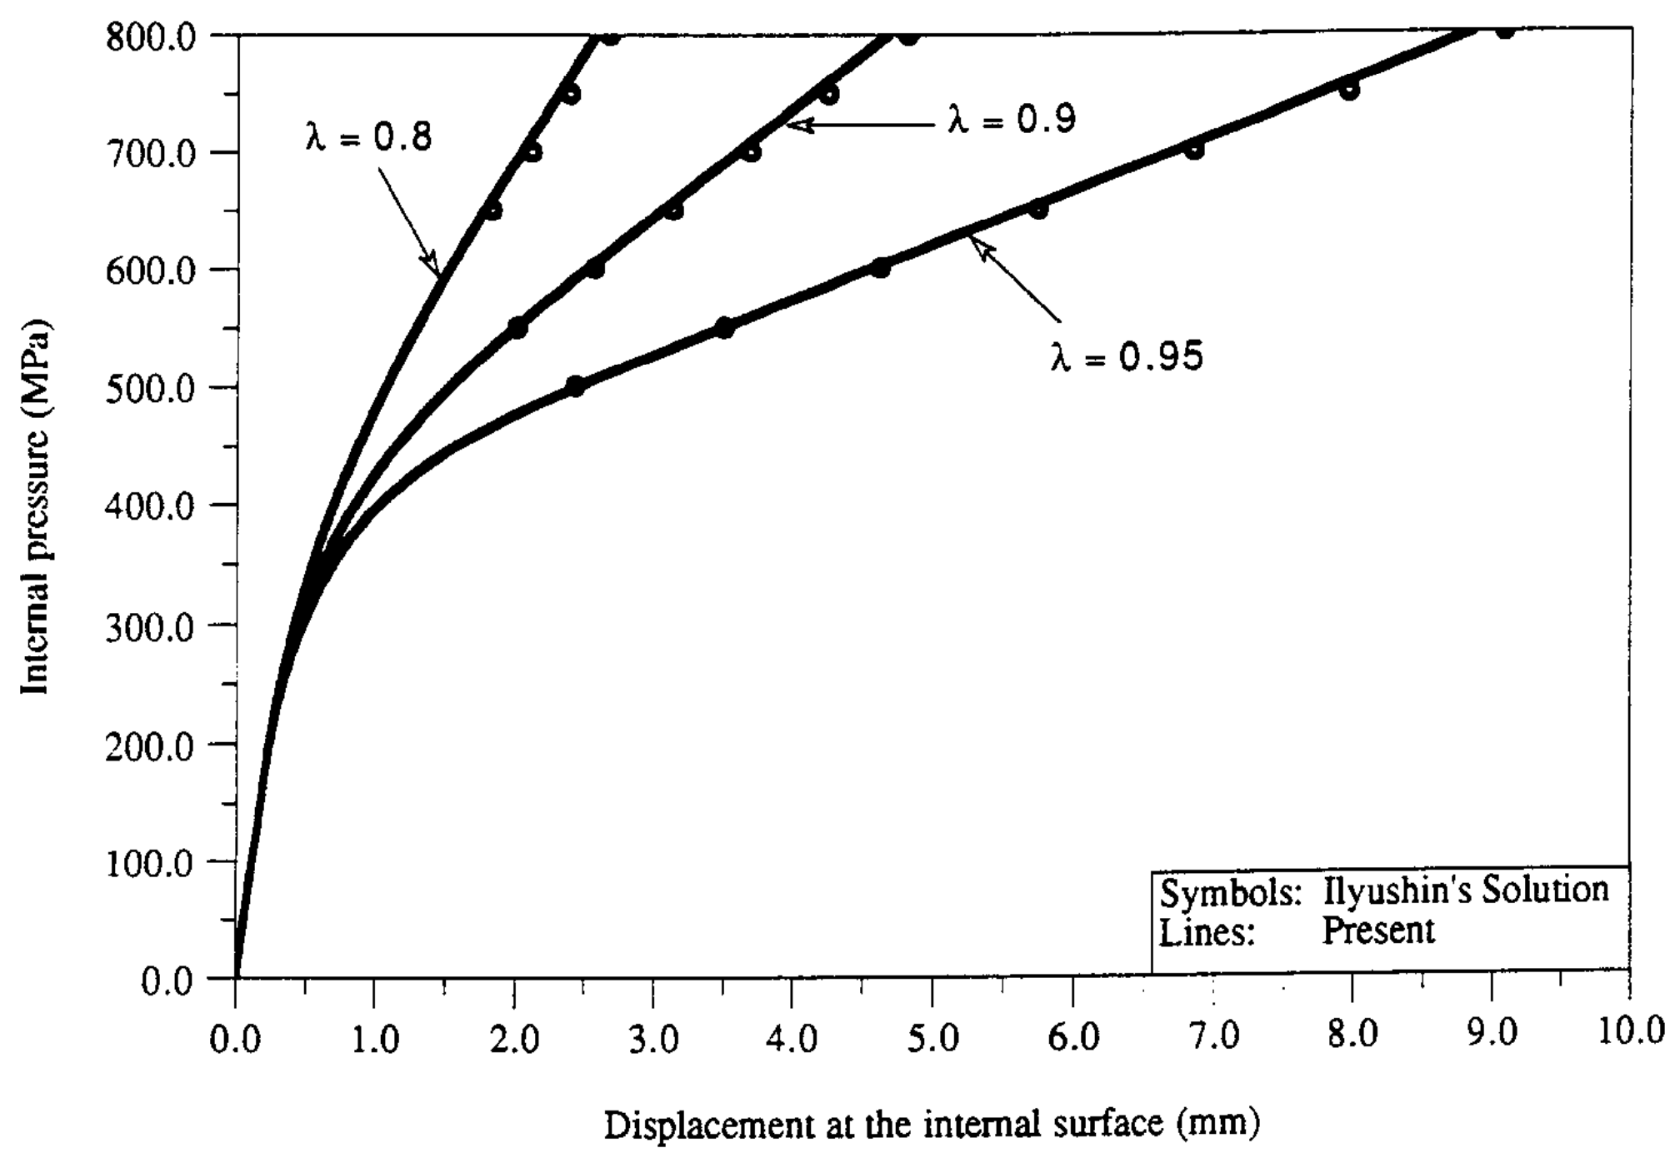
\includegraphics[width=0.8\textwidth]{\path/comparaison_ilyushin}
\caption{Réponse pression-déplacement d'une sphère creuse pour différents degrés d'écrouissage.}
\label{fig:comparaison_ilyushin}
\end{figure}
Les propriétés matérielles et géométriques choisies pour la sphère creuse sont : $\ModCis = 7,7 \times 10^4\mega\pascal$, $\BulkModulus = 1,67 \times 10^5\mega\pascal$, $\sigma_y = 300\mega\pascal$, $a = 300\milli\metre$ et $b = 600\milli\metre$. Dans les analyses effectuées, $p_{ext}$ a été maintenu constant à zéro et $p_{int}$ a été varié ; 20 points d'intégration numérique ont été utilisés le long de la direction radiale.

Comme on peut l'observer, sur la plage complètement plastique, l'accord entre les résultats théoriques et numériques est très proche. Les résultats du modèle proposé montrent une liaison régulière entre les états complètement élastique et complètement plastique. Cela ajoute une certaine crédibilité à la validité du modèle sur toute la plage élasto-plastique. Une observation intéressante qui peut être faite à partir des résultats montrés dans la \figref{fig:comparaison_ilyushin} est que la capacité de résistance à la charge de la structure augmente avec une augmentation du niveau d'écrouissage (c'est-à-dire lorsque $\lambda$ diminue). Pour les trois cas présentés, la non-linéarité due à l'écoulement du matériau commence à une pression de 200 MPa, cependant, l'état complètement plastique se développe à une pression beaucoup plus élevée (approximativement 600 MPa) pour le matériau avec $\lambda = 0,8$ comparé à celui avec $\lambda = 0,95$ pour lequel la pression correspondante est d'environ 450 MPa ; le niveau de déplacement correspondant au début de l'état complètement plastique est le même (environ 1,52 mm) pour tous les cas étudiés.

\begin{figure}[h!]
%\centering \includegraphics[width=0.8\textwidth]{\path/repartition_sigma_1_3}
\caption{Variation des contraintes induites avec la distance à différents niveaux de pression interne.}
\label{fig:repartition_sigma_1_3}
\end{figure}
L'une des forces du modèle proposé est qu'il peut générer des informations plus détaillées concernant la réponse du problème. Ceci est démontré dans la \figref{fig:repartition_sigma_1_3} qui montre la variation des composantes de contrainte $\sigma_{\theta\theta}$ et $\sigma_{rr}$ avec la distance radiale pour le cas de $\lambda = 0,95$ pour plusieurs niveaux de pression, allant de 200 à 800 MPa. Les résultats indiquent que tandis que la variation de $\sigma_{rr}$ avec la distance radiale est assez uniforme, étant la plus grande à la frontière de la pression appliquée ($r = a$) et diminuant graduellement en intensité avec la distance, la variation de $\sigma_{\theta\theta}$ est plutôt erratique. Cette irrégularité provient de la redistribution des contraintes après le premier écoulement qui se produit à $p_{int} > 200\mega\pascal$ ; après que le corps entier atteint un état complètement plastique ($p_{int} > 500\mega\pascal$) la variation de $\sigma_{\theta\theta}$ devient uniforme.
\subsection{Traction uniaxiale d'un barreau}
Nous étudions l'essai bien connu de traction uni-axial sur un barreau élasto-plastique. Le matériau a l'étude est un acier standard \eqref{eq:pte_acier_standard}.

Pour un essai de traction uniaxiale sur un barreau de section $S = l \times L$ soumis à un déplacement imposé $u_x$ conduisant à une déformation $\varepsilon = u_x/h$, le champ de contrainte est uniaxial de la forme $\SC = \sigma_{xx}\e_x \otimes \e_x$. Dans ce cas, la contrainte principale égalise la contrainte équivalente de von Mises : $\sigma_{eq} = \sigma_{xx}$.
\subsubsection{Phase élastique ($\varepsilon \leq \varepsilon_c$)}
La déformation critique marquant la limite d'élasticité est donnée par :
$$\varepsilon_c = \frac{\sigma_Y}{E}$$
En phase élastique, la relation contrainte-déformation suit la loi de Hooke :
$$\sigma_{xx} = E\varepsilon$$
La force de réaction correspondante s'exprime :
$$F = \sigma_{xx} \cdot S = E\varepsilon S$$
\subsubsection{Phase élasto-plastique ($\varepsilon > \varepsilon_c$)}
Pour un matériau avec écrouissage isotrope linéaire de module $H$, la déformation totale se décompose en parties élastique et plastique : $\varepsilon = \varepsilon_e + \varepsilon_p$.

En phase plastique, la contrainte vérifie le critère de plasticité :
$$\sigma_{xx} = \sigma_Y + H\varepsilon_p$$
La déformation élastique reste liée à la contrainte par $\varepsilon_e = \sigma_{xx}/E$, d'où :
$$\varepsilon = \frac{\sigma_{xx}}{E} + \varepsilon_p = \frac{\sigma_Y + H\varepsilon_p}{E} + \varepsilon_p$$
En résolvant pour $\sigma_{xx}$, on obtient la relation constitutive élasto-plastique :
$$\sigma_{xx} = \sigma_Y + \frac{EH}{E+H}(\varepsilon - \varepsilon_c)$$
Le module tangent élasto-plastique vaut donc :
$$E_T = \frac{EH}{E+H}$$
La force de réaction en phase plastique s'exprime finalement :
$$F = \left[\sigma_Y + E_T(\varepsilon - \varepsilon_c)\right] \cdot S$$
Cette formulation garantit la continuité à la transition élasto-plastique et respecte la décomposition additive des déformations caractéristique de la plasticité en petites déformations.

En plus des paramètres caractéristique de l'acier, nous prenons une limite d'élasticité $\SigY = 200\mega\pascal$ et un module d'écrouissage isotrope $H=E/10$. La comparaison analytique-numérique est présentée à la \figref{fig:comparaison_SOD}.
\begin{figure}[h!]
\centering 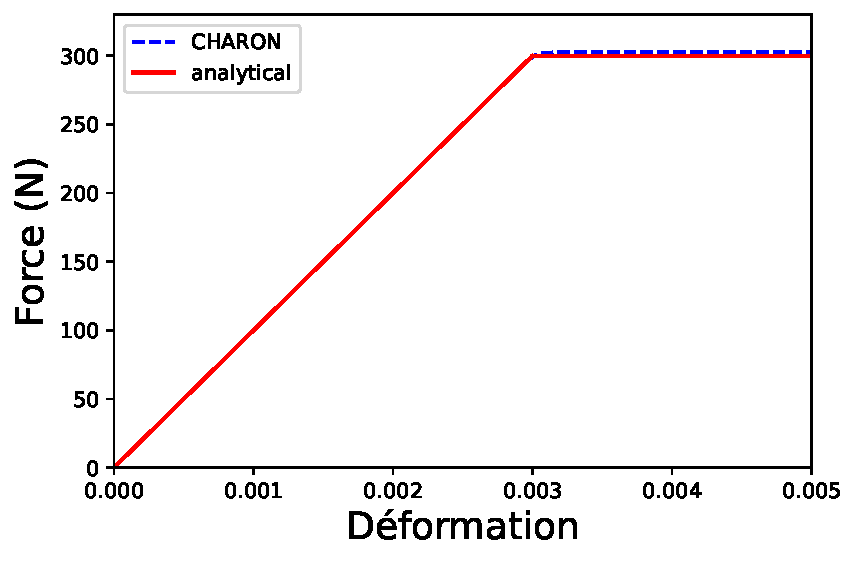
\includegraphics[width=0.8\textwidth]{\path/Traction_3D_elasto_plast}
\caption{Traction d'un barreau élasto-plastique avec un modèle tridimensionnel}
\label{fig:comparaison_SOD}
\end{figure}
\section{Endommagement}
\subsection{Rupture fragile par champ de phase}
\ToDo{}
\subsubsection{Traction unidimensionnelle}
\ToDo{}
\subsubsection{Dilatation sphérique}
\ToDo{}
\subsection{Rupture ductile avec le modèle de Johnson}
Nous étudions la croissance d'un pore isolé dans le cadre du modèle de Johnson. 
\subsubsection{Solution analytique du modèle de Johnson}
\ToDo{}
\subsubsection{Convergence du modèle de Johnson dynamique}
\chapter{Comparaison de codes}\label{Chapitre:Comparaison autres codes}
\section{Comparaison avec Abaqus CAE}
\ToDo{Faire toutes les comparaisons là où il n'y a pas de solution analytique}
\section{Comparaison avec des codes internes}
Pour tous les cas 0.1 en linéaire et 1 en quadratique, pas de pseudo en détente.
\subsection{Tubes à choc de Sod}
Nous reprenons l’expérience du tube à choc de Sod. Le matériau a l'étude est un gaz parfait (eos afférente et déviateur nul). Les paramètres sont les suivants: $\gamma= 1.4$, $C_{v}=\dfrac{R}{\gamma-1}=20.795$. Concernant la masse volumique et la température initiale celles-ci sont représentés sur la FIGREF
$\rho_{0} = 1$, $\rho_{0}=0.125$, 
Cet essai va nous permettre de valider la convergence en temps et en espace. Nous allons d'abord tester un pas de temps fixe plus petit que la CFL puis laisser CHARON et MaHyCo calculer leurs propres incréments de temps.

Nous allons ensuite comparer l'influence du type d'éléments finis utilisé pour représenter la structure. Avec le code CHARON, nous mettrons à l'épreuve les éléments \emph{Continuous Galerkin}  à  interpolation linéaire et quadratique. Pour le maillage régulier, interpolation  linéaire et quadratique, regarder quel maillage quadratique donne le même résultat. $200$ éléments dans la largeur pour le modèle $1D$ et modèle 2D plan avec $200 \times 10$ et coupe au milieux.

\subsection{Choc avec rampe}
On applique une rampe de pression pour $t \in [0, 1e-7]$ avec $pente = 3e17$ jusqu'à une pression max de $3\giga \pascal$ matériau à l'étude alu:
EOS Mie Gruneisen: 
$\gamma_{0}=2$, $C=7.905e10$ coefficient linéaire, $D = 1.3266e11$, coefficient quadratique $S=0$ coefficient cubique. Maillage $100*10$ pour du 2D et refaire pour 1D. $\rho_{0} = 2700\kilo\gram\per\metre^{3}$. $T_{fin}=2e-7\second$
\subsubsection{Cas hydro pure}
\subsubsection{Cas élasto}
 Comparer avec les deux lois déviatorique $\mu=30\giga\pascal$, HPP et Néo-Hook.
\subsection{Cas élasto-plastique}
$\sig_{Y}=40\mega\pascal$, plasticité parfaite éventuellement puis avec $H=7\giga\pascal$ puis comparaison avec plasticité grande def.
\subsection{Choc concentrique}
quart de disque en axi avec vitesse imposée sur le bord (déplacement linéaire en temps) en 1D et 2D. Eos U1, U5, U8 avec $\kappa= 60\giga\pascal$. Plusieurs maillage généré avec gmsh fourni par JPP.
\subsection{Cas test de Noh}
Le choc concentrique peut être remplacé par ce cas test de noh

\subsection{Test de Taylor}
Mise en vitesse d'un cylindre qui vient s'écraser sur une paroi (forme une espèce de patte d'éléphant) en 2D plan, 2D axi, 3D. $E=117\giga\pascal$, $H=100\mega\pascal$ $\nu=0.35$ $\mu = \dfrac{E}{2(1+\nu)}$, $\kappa = \dfrac{E}{3(1-2\nu)}$, $v_{0}=227\metre\per\second$, $r=3.2\milli\metre$, $h=32.4\milli\metre$. avec eos U1. $\rho_{0} = 8930\kilo\gram\per\metre^{3}$ $\sigma_{Y} = 400\mega\pascal$.  Maillage 30 en hauteur, et rayon intérieur 5-6 mailles dans rayon. Maillage fourni
Résultats à $T_{fin} =80\micro\second$, rayon patte d'éléphant $7.127\milli\metre$.
\subsection{Cas test de Sedof}
TODO
A coder pour CHARON: interface avec gmsh, possibilité de mettre une vitesse initiale, 
\section{Plasticité écrouissage isotrope FEniCS}
\subsubsection{Implémentation}
Le problème considéré est celui d'un cylindre creux en déformation plane de rayon interne (resp. externe) $R_i$ (resp. $R_e$) sous pression interne uniforme $q$.

Nous commençons par importer les modules pertinents et définir certaines constantes géométriques.

Nous modélisons ensuite un quart de cylindre à l'aide de Gmsh de manière similaire à la démo.

Nous définissons maintenant quelques paramètres matériels et l'espace des fonctions pour le champ de déplacement. Nous choisissons ici un espace Lagrange standard $\mathbb{P}_2$.

{attention}
Les calculs élasto-plastiques peuvent entraîner des problèmes de verrouillage volumétrique induits par des déformations plastiques incompressibles. Dans cette démo, nous n'essayons pas de résoudre ce problème et utilisons des triangles quadratiques qui, en 2D, sont suffisants pour atténuer le phénomène de verrouillage.

Les conditions aux limites correspondent à des conditions de symétrie sur les parties inférieure et gauche (resp. numérotées 1 et 2). La charge consiste en une pression uniforme sur la frontière interne (numérotée 3). Elle sera progressivement augmentée de 0 à une valeur légèrement supérieure à $q_\text{lim}=\dfrac{2}{\sqrt{3}}\sigma_0\log\left(\dfrac{R_e}{R_i}\right)$, qui est la charge limite analytique pour un matériau parfaitement plastique (sans durcissement).
\subsubsection{Variables d'état internes et éléments Quadrature}
Lorsqu'on travaille avec des modèles constitutifs non linéaires, des variables d'état internes telles que les déformations plastiques doivent représenter l'historique vu par le matériau et doivent être stockées d'une manière ou d'une autre. Nous choisissons ici de les représenter à l'aide d'éléments Quadrature. Ce choix permettra d'exprimer l'équation constitutive matérielle non linéaire aux points de Gauss uniquement, sans impliquer aucune interpolation d'expressions non linéaires à travers l'élément. Cela assurera un taux de convergence optimal pour la méthode de Newton-Raphson, voir chap. 26 de {cite:p}logg2012fenicsbook. Nous aurons besoin d'éléments Quadrature pour des vecteurs de dimension 4 et des scalaires, le nombre de points de Gauss sera déterminé par le degré requis deg\_quad de l'élément Quadrature, voir la présentation pour plus de détails sur le choix des règles de quadrature.

{note}
Nous soulignons que, bien que le problème soit en 2D, les déformations plastiques surviennent également dans la direction transversale $zz$. Cela nécessitera de suivre les composantes $zz$ hors plan des états de contrainte/déformation.
Diverses fonctions sont définies pour suivre l'état interne actuel et les incréments actuellement calculés.

Avant d'écrire la forme variationnelle, nous définissons maintenant certaines fonctions utiles qui permettront de réaliser la mise à jour de la relation constitutive en utilisant la procédure de retour radial décrite précédemment. Tout d'abord, le tenseur de déformation sera représenté de manière tridimensionnelle en ajoutant des zéros sur les composantes hors plan puisque, même si le problème est en 2D, la relation constitutive plastique impliquera des déformations plastiques hors plan. La relation constitutive élastique est également définie et une fonction as\_3D\_tensor permettra de représenter un vecteur de dimension 4 contenant respectivement les composantes $xx, yy, zz$ et $xy$ sous forme d'un tenseur 3D :

La procédure de retour radial est mise en œuvre dans la fonction constitutive\_update qui prend comme argument une incrémentation totale de la déformation $\Delta\varepsilon$, l'état de contrainte précédent old\_sig et la déformation plastique précédente old\_p. Pour calculer l'incrément de déformation plastique, nous utilisons la formule {eq}Deltap-formula où ppos implémente la fonction de partie positive.

L'évolution plastique nécessite également le calcul du vecteur normal à la surface de rupture finale donné par $\boldsymbol{n}{\text{elas}} = \devia\text{elas}/\sigma_{eq}^{\text{elas}}$. Dans ce qui suit, ce vecteur doit être nul en cas d'évolution élastique. Par conséquent, nous le multiplions par $\dfrac{\langle f_{\text{elas}}\rangle_+}{ f_{\text{elas}}}$ pour traiter les deux cas en une seule expression. L'état de contrainte final est corrigé par la déformation plastique comme suit $\SC_{n+1} = \SC_{\text{elas}} - \beta \devia_\text{elas}$ avec $\beta = \dfrac{3\mu}{\sigma_{eq}^{\text{elas}}}\Delta p$. On peut observer que le dernier terme disparaît en cas d'évolution élastique de sorte que la contrainte finale est en effet le prédicteur élastique.

Afin d'utiliser une procédure de Newton-Raphson pour résoudre l'équilibre global, nous devons également dériver la matrice tangente algorithmique cohérente donnée par :
$$\CC_{\text{tang}}^{\text{alg}} = \CC - 3\mu\left(\dfrac{3\mu}{3\mu+H}-\beta\right)  \boldsymbol{n}_{\text{elas}} \otimes \boldsymbol{n}_{\text{elas}} - 2\mu\beta\mathbb{Dev}$$
où $\mathbb{Dev}$ est le tenseur du quatrième ordre associé à l'opérateur déviatoire (notez que $\CC_{\text{tang}}^{\text{alg}}=\CC$ pour l'évolution élastique). Contrairement à ce qui est fait dans {cite:p}logg2012fenicsbook, nous ne le stockons pas sous forme des composantes d'un tenseur du quatrième ordre, mais il suffira de suivre le vecteur normal et le paramètre $\beta$ lié aux déformations plastiques. Nous définissons plutôt la fonction sigma\_tang calculant la contrainte tangente $\SC_\text{tang} = \CC_{\text{tang}}^{\text{alg}}: \boldsymbol{\varepsilon}$ comme suit :

{attention}
Dans ce cas simple, l'expression de la contrainte de constitutive\_update est explicite et peut être représentée à l'aide d'expressions pures de ufl. Ainsi, nous pourrions utiliser cette expression non linéaire dans la résiduelle non linéaire et utiliser la différentiation automatique pour calculer directement la forme tangente correspondante. Ici, nous faisons délibérément différemment, comme une approche pédagogique vers des modèles constitutifs plus complexes pour lesquels l'expression de la contrainte n'est plus explicite. Dans ces cas, la contrainte et la rigidité tangentielle doivent être formellement représentées aux points de quadrature et la constitutive\_update fournit les valeurs correspondantes aux points de quadrature.
\subsubsection{Problème global et procédure personnalisée de Newton-Raphson}
Nous sommes maintenant en mesure de définir la forme variationnelle de la résiduelle non linéaire et la forme bilinéaire tangente correspondante à utiliser dans un schéma global de Newton-Raphson. Chaque itération nécessitera d'établir l'équilibre en ramenant à zéro la résiduelle entre les forces internes associées à l'état de contrainte actuel sig et le vecteur de force externe. Comme nous utilisons des éléments Quadrature, une mesure d'intégration personnalisée dx doit être définie pour correspondre au degré et au schéma de quadrature utilisés par les éléments Quadrature.

Pendant les itérations de Newton-Raphson, nous devrons interpoler certaines expressions ufl aux points de quadrature pour mettre à jour les fonctions correspondantes. Nous définissons la fonction interpolate\_quadrature pour le faire. Nous obtenons d'abord l'emplacement des points de quadrature dans l'élément de référence, puis utilisons fem.Expression.eval pour évaluer l'expression sur toutes les cellules.

Nous définissons maintenant la boucle globale de Newton-Raphson. À chaque itération, nous devons résoudre un système linéaire de la forme :
$$\mathbf{A}_\text{tang}\mathbf{\d u} = -\mathbf{R}$$
où $\mathbf{R}$ est la valeur actuelle de la résiduelle non linéaire, $\mathbf{du}$ la correction d'itération au champ inconnu $\mathbf{u}$ et $\mathbf{A}_\text{tang}$ l'opérateur tangent de la résiduelle non linéaire. Pour simplifier la mise en œuvre, nous nous appuyons sur la classe utilitaire fem.petsc.LinearProblem pour définir et résoudre les problèmes linéaires. Dans ce qui suit, nous devons explicitement séparer les étapes où nous assemblons le côté droit du système linéaire de celles où nous assemblons la matrice du côté gauche et résolvons le système linéaire. Nous définissons donc une nouvelle classe héritant de LinearProblem et séparant ces différentes étapes.

Nous discrétisons la charge appliquée en utilisant NodalLoadControl. Cela nous permet de contrôler la charge sur un seul nœud plutôt que sur toute la frontière externe.

Enfin, nous pouvons exécuter la boucle de Newton-Raphson en augmentant progressivement la charge externe. La démo affiche le chargement, les déplacements maximaux et les résidus de Newton-Raphson à chaque itération.

\chapter{Structure du code CHARON}\label{Chapitre:Structure du code CHARON}
\section*{Introduction FEniCSx}
La librairie FEniCSx est une collection de package dédiée à la résolution simplifiée d'équations aux dérivées partielles. Le projet est conduit depuis 2003 par de nombreuses universités Chicago, Chalmers etc...

La résolution des équations aux dérivées partielles résulte d'une discrétisation du problème, puis le calcul d'une solution approchée par la méthode des éléments finis. L'accent a été placé tôt sur la parallélisation et le calcul haute performance grâce à l'intégration de la librairie PETSc pour les calculs d'algèbre linéaire. L'interface est codée en python et dispose d'un vocabulaire haut niveau extrêmement concis permettant de conserver une syntaxe proche de l'écriture mathématiques du problème.

Une liste, non exhaustive, des sous-composants majeurs est la suivante:
\begin{itemize}
\item Basix génère des éléments finis d'ordre arbitraire,
\item UFL (Unified Form Language) implémente avec un vocabulaire simple les formes linéaires issues de la formulation variationnelle (grâce à ce package, les opérateurs divergence, rotationnel, transposition, déterminant etc.. sont manipulables par l'utilisateur).
\item UFCx (Unified Form compiler), interface bas niveau écrite en C++ qui permet l'évaluation et l'assemblage des formes linéaires (par exemple la création de la matrice de rigidité).
\item FFCx (FEniCS Form Compilerx), compilateur \og just in time \fg{} réalisant la transition UFL $\rightarrow$ UFCx
\item Dolfinx, librairie C++/Python incluant des algorithmes d'assemblages de formulations discrétisées, de manipulation de maillage etc...
\end{itemize}
\section{Structure générale du code}
Le code CHARON (Code Hydrodynamique Anelastique en explicite Rapide avec dOlfiN) est un package python utilisant la librairie éléments finis FEniCSx afin de résoudre par la méthode des éléments finis les problèmes mécaniques. Sa structure générale est ici détaillée.\\

Le code repose sur trois grands blocs (voir \Figref{fig:Structure_code_CHARON}):
\begin{itemize}[label=$\dagger$]
\item Le premier (voir détails \subsecref{Subsection:Charon Formulation variationnelle}) définit le modèle mécanique, c'est-à-dire la formulation variationnelle du problème. Celle-ci est en toute généralité posée sur un solide tridimensionnel puis dégénérée éventuellement en modèle réduit (1D ou 2D).
\item Le deuxième bloc (voir détails \subsecref{Subsection:Charon Loi de comportement}) précise la loi de comportement, c'est-à-dire la relation entre la contrainte tridimensionnelle de Cauchy $\SC$ aux variables température $T$, déplacement $\Dep$ et variables internes $\balpha$.
\item Enfin, le bloc de résolution (voir détails \subsecref{Subsection:Charon Solveur}) permet la résolution du problème mécanique défini par la formulation variationnelle et la loi de comportement.
\end{itemize}
Les différents blocs et leurs sous fichiers vont maintenant être détaillés
\subsection{Formulation variationnelle}\label{Subsection:Charon Formulation variationnelle}
Cette partie est constituée des fichiers suivants:
\begin{itemize}
\item problem.py est le fichier principal qui permet de définir le problème mécanique, c'est-à-dire les paramètres d'études (analyse statique ou dynamique, présence de non-linéarités, etc..) mais aussi la définition des espaces fonctionnelles et la formulation variationnelle.
\item unidimensional.py est un fichier qui  particularise le problème 3D à un cas unidimensionnel (cartésien, cylindrique ou sphérique). La forme particulière postulée du champ de déplacement permet de proposer des expressions simplifiées pour le gradient de la transformation et de ramener l'étude à un maillage 1D.
\item De même, bidimensional.py rassemble les routines pour réduire aux études 2D (déformation plane et axisymétrique).
\item tridimensional.py contient enfin les fonctions nécessaires à la formulation 3D la plus générale.
\end{itemize}

\subsection{Loi de comportement}\label{Subsection:Charon Loi de comportement}
Il s'agit certainement du bloc amené susceptible d'être modifié par l'utilisateur. Il est constitué de plusieurs fichiers traitant séparément l'élasticité, la plasticité et l'endommagement.
\begin{itemize}
\item ConstitutiveLaw.py est le fichier majeur, il définit un objet \og constitutive \fg{}, lequel possède des attributs correspondant aux différents comportements (élastique, plastique et endommageable).
\item elastic.py contient les différentes lois d'élasticité, formulées à l'échelle tridimensionnelle. L'ajout d'une loi élastique par l'utilisateur est possible, pourvu que ses arguments soient: la température, le gradient du champ de déplacement, le gradient du champ des vitesses et le jacobien de la transformation.
\item plastic.py contient les différents modèles de plasticité. Là est défini par exemple le type de variable plastique (scalaire, tensorielle), mais aussi la fonction de charge, l'écrouissage etc...
\item damage.py concatène les modèles d'endommagement et de cavitation (comme celui de Johnson). Comme précédemment la variable d'endommagement ainsi que sa loi d'évolution sont précisées dans ce fichier.
\end{itemize}
\subsection{Solveur}\label{Subsection:Charon Solveur}
Le problème mécanique correctement défini est ensuite donné en argument au solveur qui résout séquentiellement: l'équilibre, la thermique, la plasticité et enfin l'endommagement. Le caractère explicite de la résolution découple les différentes non linéarités.
\begin{itemize}
\item le fichier Solve.py implémente la boucle d'incrémentation temporelle pour la résolution dynamique. A l'intérieur de cette boucle, sont appelés les autres solveurs.
\item displacement\_solver.py code la résolution en déplacement explicite d'ordre 2,
\item energy\_solver actualise la température par un schéma également explicite,
\item plastic\_solve actualise l'endommagement plastique.
\item Le fichier DamageSolve.py contient l'outil de résolution de l'endommagement. 
\end{itemize}

\subsection{Fichiers annexes}
Quelques fichiers plus génériques, appelés par un ou plusieurs blocs ci-dessus sont consignés à l’extérieur. Nous donnons par exemple:
\begin{itemize}
\item default\_parameters.py inclut les paramètres par défaut (degrés des éléments finis, précision des solveurs non-linéaires etc...)
\item generic\_functions.py rassemble un certain nombre de fonctions génériques (maximum entre deux vecteurs, opérateur \og partie positive \fg{} etc...)
\end{itemize}
\section{Résolution d'EDO}
La résolution d'équation différentielle ordinaire (EDO) est assuré par la bibliothèque Diffrax, sous projet de la librairie JAX. 
\section{Latitude laissée aux développeurs}
Le code CHARON ambitionne à laisser une grande liberté aux développeurs pour expérimenter de nouvelles lois de comportement, d'évolution chimique etc\dots. Cette modularité est permise par le caractère générique du code et le découpage en plusieurs classes indépendantes. Le changement d'une loi, pourvu qu'elle respecte une certaine nomenclature, n'impacte pas la résolution ultérieure. Les noms de classes sont explicites et indiquent autant que se peut où doivent être placées les éventuelles modifications apportées au code. Si un développeur souhaite modifier les propriétés élasto-plastique d'un matériau, il pourra par exemple préciser l'existence d'une nouvelle variable plastique et son impact sur la contrainte dans la classe \og PlasticProblem \fg{}. Puis, à chaque itération, l'évolution de la variable plastique en fonction des champs mécanique précédemment trouvés devra être spécifiée dans la classe \og PlasticSolve \fg{}.
\section{Problème locaux et non locaux}
Le code CHARON résout plusieurs problèmes de physique qu'il est possible de scinder en deux catégories:
\begin{itemize}[label = $\star$]
\item Les problèmes non locaux, caractérisés par des équations aux dérivées partielles qui mettent en jeu par exemple les gradients, divergences ou laplaciens des champs inconnus. Ces problèmes non locaux sont résolus par la méthode des éléments finis et les inconnues sont des \textbf{Function} définies \textbf{aux nœuds du maillage}. La plupart de ces champs sont discrétisés par des éléments finis de Lagrange à interpolation linéaire ou quadratique. On pourra citer par exemple:
\begin{itemize}
\item le déplacement $\Dep$ qui est solution de l'équation de conservation de la quantité de mouvement, 
\item la température $T$ \textbf{si la diffusion thermique est prise en compte},
\item l'endommagement $d$ si la rupture est pilotée par la méthode de champ de phase.
\end{itemize}
Dans les exemples ci-dessus, des conditions aux limites sont nécessaires pour résoudre le problème variationnel et sont de deux types:
\begin{itemize}
\item Les conditions aux limites de Dirichlet qui imposent directement la valeur des champs au bord. 
\item Les conditions aux limites de Neumann qui imposent la valeur des gradients.
\end{itemize}
Par exemple pour le champ de déplacement, il est possible soit d'imposer la valeur de $\Dep$ au bord soit la contrainte $\SC$. Si l'utilisateur ne mentionne rien, des conditions aux limites de Neumann homogènes sont alors appliquées (bord libre correspondant à une contrainte nulle pour le champ de déplacement et bord calorifugé (flux nul) pour la température.  
\item Parallèlement à cela CHARON calcul un certain nombre de champs dont l'évolution est piloté par un critère local. On pourra penser à:
\begin{itemize}
\item l'évolution des concentrations $c$ des phases, 
\item la porosité dans le modèle de rupture de Johnson, 
\item la déformation plastique $\DefoHPP^{p}$,
\item la température dans le cas d'une transformation \textbf{adiabatique} (pas de terme $\Delta T$ dans l'équation de la chaleur),
\item la pression si on retient une loi d'état tabulée.
\end{itemize}
Tous ces champs sont alors représentés par des \textbf{Function} définies \textbf{aux points de Gauss}, c'est à dire des fonctions de type \textbf{quadrature}. Aucune condition aux limites n'est dans ce cas imposée.
\end{itemize}
\section{FAQ}
\begin{center}
\emph{J'aimerais connaître la valeur de ma fonction ?}
\end{center}
\begin{itemize}
\item S'il s'agit d'une \emph{Fonction} FEniCS (telle que le champ de déplacement, de température d'endommagement etc..) il est possible d'accéder aux valeurs aux nœuds de la fonction en tapant: 
\begin{center}
nom\_de\_ma\_fonction.vector.array
\end{center}
\item S'il s'agit d'une \emph{Expression} (combinaison d'autres fonctions, opérateurs différentiels etc..) il est nécessaire d'abord de projeter l'expression sur un espace fonctionnel approprié. Par exemple si l'on a défini un champ constant par élément, on peut alors définir une fonction $f_{quad}$ de type \emph{Quadrature} puis d'interpoler l'expression dont on veut avoir la valeur sur cette fonction $f_{quad}$.
\begin{center}
\begin{tabular}{l}
V = quad.quadrature\_space(["Scalar"])\\
Expr = Expression(nom\_de\_mon\_expression, V.element.interpolation\_points()\\
$f_{quad}$  = Function(V)\\
$f_{quad}$.interpolate(Expr)\\
print($f_{quad}$.vector.array)
\end{tabular}
\end{center}
\end{itemize}
\section{Les commandes utiles dans FEniCSx}
\begin{itemize}
\item Les espaces fonctionnels Function Space
\item Les fonctions
\begin{itemize}
\item Les attributs vectors d'une fonction
\item La méthode interpolate d'une fonction
\end{itemize}
\item Les mesures d'intégration
\item Les formes variationnelles 
\ToDo{A finir}
\end{itemize}
\begin{appendices}
\chapter{Exercices de prise en main}
%\section{Exercices de prise en main}
%\ToDo{Créer un exercice qui mixerait les différents exemples du premier chapitre}
\section{Exercices développeurs}\label{Section:Exercices développeurs}
\begin{Exercice}{Loi d'état de Vinet} Proposer une méthode pour implémenter la loi d'état de Vinet:
$$p=3K_{0}x^{-2}(1-x)e^{\frac{3}{2}(K_{0}'-1)(1-x)} \avec x=\left(\dfrac{\rho_{0}}{\rho}\right)^{\frac{1}{3}}$$
On remarquera que cette loi ne prend pas en compte la température.
\end{Exercice}
\begin{Correction}{
L'implémentation d'une nouvelle loi d'état s'opère en deux étapes. La première consiste à définir une nouvelle classe dans le fichier material.py contenant les constantes caractéristiques du matériau (ici les deux coefficients $K_{0}$, $K_{0}'$ ainsi que la masse volumique initiale $\rho_{0}$). En plus de cela il est nécessaire de fournir une estimation de la célérité des ondes élastiques pour que CHARON puisse calculer le pas de temps vérifiant la condition CFL. Ici, nous estimons par exemple cette célérité via:
$$c\approx \dfrac{\partial p}{\partial \rho}(\rho=\rho_{0})$$
Or:
$$\begin{aligned}
&\dfrac{\partial P}{\partial \rho}=\dfrac{\partial P}{\partial x}\dfrac{\partial x}{\partial \rho}=e^{\frac{3}{2}(K_{0}'-1)(1-x)}\left[-\dfrac{3}{2}(K_{0}'-1)\left(3K_{0}x^{-2}(1-x)\right)-6K_{0}x^{-3}(1-x)-3K_{0}x^{-2}\right]\left[-\dfrac{\rho_{0}^{\frac{1}{3}}}{3\rho^{\frac{4}{3}}}\right]\\
\implique &\dfrac{\partial P}{\partial \rho}(\rho_{0})=\dfrac{\partial P}{\partial x}(x=1)\dfrac{\partial x}{\partial \rho}(\rho=\rho_{0})=\dfrac{K_{0}}{\rho_{0}}\\
\implique &c=\sqrt{\dfrac{K_{0}}{\rho_{0}}}
\end{aligned}$$
}\end{Correction}

\begin{Exercice}{Loi fluide visco-élastique} Une loi de comportement simple pour décrire un fluide visco-élastique est donnée par:
$$\begin{aligned}
\SC&=-p(\rho)\tenMetrique+2\eta(\rho)\dev\TD+\kappa(\rho)\tr(\TD)\tenMetrique\\
\eta(\rho)&=\eta_{0}\exp\left(C_{1}\rho^{C_{2}}\right)
\end{aligned}$$
On remarquera que cette loi ne prend pas en compte la température.
\end{Exercice}
\begin{Correction}{Il est tout d'abord nécessaire  de créer un nouveau matériau avec les paramètres $\eta_{0}$, $C_{1}$, $C_{2}$ ainsi qu'une estimation de la vitesse, puis il est possible simplement d'implémenter une nouvelle loi élastique dans élastique.py avec la loi de comportement sus-mentionnée. Une relation entre la température et l'énergie interne doit être précisée sans quoi l'évolution sera nécessairement isotherme.}\end{Correction}
\chapter{Utilisation de CHARON sur le calculateur Exa}
\section{Utilisation de CharonX sur calculateur}
\subsection{Configuration initiale}
Placer le code CharonX dans un dossier \texttt{charon} sur le home du calculateur exa\footnote{Actuellement le code FEniCSx est uniquement installé sur le calculateur.}. Pour accéder à exa, taper dans une fenêtre de commande:
\begin{equation}
\blue{\text{ssh -Y exa}}
\label{eq:init_exa}
\end{equation}
\begin{Rem}{L'option -Y : \texttt{ssh -Y exa} sert à pouvoir avoir un affichage graphique sur la station.}\end{Rem}
Pour visualiser et modifier le fichier \texttt{.bashrc} (fichier texte exécuté par défaut au démarrage d'une session):
\begin{center}
\texttt{vi .bashrc}
\end{center}
Modifier ce fichier en rajoutant:
\begin{center}
\texttt{alias initcharon="module load gnu/11 mpi/openmpi/4.0.5 python3/3.11.4 \&\& export PYTHONPATH=\$PYTHONPATH:\${HOME}/charon/"}
\end{center}
Cette commande permettra à chaque fois que l'on tape \textcolor{blue}{initcharon} de charger les modules nécessaires et de configurer le \texttt{PYTHONPATH}.
\begin{Rem}{Pour les utilisateurs utilisant souvent exa, des conflits de modules peuvent apparaître. Il peut donc être nécessaire de purger les modules et les différents chemins en appliquant la commande:
\begin{center}
\texttt{module purge}
\end{center}
avant d'initialiser CharonX.
}\end{Rem}
Quelques commandes utiles pour vi:
\begin{itemize}
\item Pour sauvegarder le \texttt{.bashrc} dans vi: Échap puis \texttt{:wq}
\item Pour quitter sans sauvegarde: Échap puis \texttt{:q!}
\item Pour entrer en mode édition: \texttt{i}
\item Pour copier une ligne: \texttt{yy}
\item Pour coller: \texttt{p}
\item Pour supprimer une ligne: \texttt{dd}
\end{itemize}
Après avoir modifié le \texttt{.bashrc}, exécuter:
\begin{center}
\texttt{source .bashrc}
\end{center}
Puis initialiser CharonX:
\begin{equation}
\blue{\text{initcharon}}
\label{eq:init_charon}
\end{equation}
On peut ensuite lancer une console ipython et tester l'importation des modules:
\begin{verbatim}
import dolfinx
import CharonX
\end{verbatim}
\subsection{Configuration du montage distant}
En dehors d'exa, ouvrir le \texttt{.bashrc} et ajouter:
\begin{verbatim}
alias mnt='ccc_calc_sshfs -m'
\end{verbatim}
Pour trouver le chemin vers charon sur exa, se connecter à exa et taper:
\begin{verbatim}
pwd
\end{verbatim}
Cela donnera un chemin du style \texttt{/ccc/cont001/home/wf/...}

De retour sur la machine locale, dans le dossier \texttt{Desktop}, créer un lien symbolique:
\begin{verbatim}
ln -s /chemin/trouve/sur/exa Nom_du_dossier_local
\end{verbatim}
\subsection{Connexions ultérieures}
Pour lancer un calcul ultérieurement sur CharonX:
\begin{enumerate}
\item Se connecter à exa (\ref{eq:init_exa})
\item Initialiser CharonX (\ref{eq:init_charon})
\item Lancer le script Python souhaité
\end{enumerate}
\subsection{Copie de dossiers depuis une station locale}
Pour copier un dossier depuis la station locale vers le calculateur (par exemple pour mettre à jour CharonX):
\begin{verbatim}
cd /ccc/cont001/home/l2/bouteill4s
cp -r ~/charon/CharonX .
\end{verbatim}
\begin{itemize}
\item L'option \texttt{-r} permet de copier récursivement les dossiers.
\item Le symbole \texttt{\~{}} représente le dossier home de l'utilisateur sur la station locale.
\item Le point \texttt{.} à la fin indique de copier dans le dossier courant sur exa.
\end{itemize}
\subsection{Utilisation d'Emacs}
Emacs est un éditeur de texte puissant et extensible, particulièrement apprécié des développeurs. Voici un guide rapide pour son utilisation:
\\\bigskip\begin{minipage}[t]{.54\linewidth}
\textbf{Commandes de base}
\begin{itemize}
\item \textbf{Ctrl+x Ctrl+s} : Sauvegarder le fichier
\item \textbf{Ctrl+x Ctrl+c} : Quitter Emacs
\item \textbf{Ctrl+g} : Annuler la commande en cours
\item \textbf{Ctrl+x Ctrl+f} : Ouvrir un fichier
\item \textbf{Ctrl+s} : Recherche incrémentale vers l'avant
\item \textbf{Ctrl+r} : Recherche incrémentale vers l'arrière
\end{itemize}
\end{minipage}\hfill
\begin{minipage}[t]{.44\linewidth}
\textbf{Navigation}
\begin{itemize}
\item \textbf{Ctrl+a} : Aller au début de la ligne
\item \textbf{Ctrl+e} : Aller à la fin de la ligne
\item \textbf{Ctrl+v} : Page suivante
\item \textbf{Alt+v} : Page précédente
\item \textbf{Alt+<} : Début du fichier
\item \textbf{Alt+>} : Fin du fichier
\end{itemize}
\end{minipage}
\\\bigskip\begin{minipage}[t]{.46\linewidth}
\textbf{Édition}
\begin{itemize}
\item \textbf{Ctrl+d} : Supprimer le caractère sous le curseur
\item \textbf{Ctrl+k} : Couper jusqu'à la fin de la ligne
\item \textbf{Ctrl+y} : Coller
\item \textbf{Ctrl+space} : Commencer la sélection
\item \textbf{Ctrl+w} : Couper la sélection
\item \textbf{Alt+w} : Copier la sélection
\end{itemize}
\end{minipage}\hfill
\begin{minipage}[t]{.52\linewidth}
\textbf{Fenêtres et buffers}
\begin{itemize}
\item \textbf{Ctrl+x 2} : Diviser la fenêtre horizontalement
\item \textbf{Ctrl+x 3} : Diviser la fenêtre verticalement
\item \textbf{Ctrl+x o} : Passer à l'autre fenêtre
\item \textbf{Ctrl+x 1} : Garder uniquement la fenêtre courante
\item \textbf{Ctrl+x b} : Changer de buffer
\item \textbf{Ctrl+x k} : Fermer un buffer
\end{itemize}
\end{minipage}
Emacs dispose également de nombreux modes spécialisés pour différents langages de programmation, offrant des fonctionnalités telles que la coloration syntaxique, l'indentation automatique et la complétion de code. Nous conseillons pour la fatigue des yeux de changer les paramètres de thème par défaut et d'opter pour le thème wombat.
\subsection{Création d'alias}
Pour créer des alias personnalisés:
\begin{verbatim}
emacs .alias
\end{verbatim}
Ajouter des alias sous la forme:
\begin{verbatim}
alias nom_de_l_alias='commande'
\end{verbatim}
Par exemple:
\begin{verbatim}
alias ll='ls -la'
alias py='python3'
alias jupyterlab='jupyter lab --no-browser'
\end{verbatim}
N'oubliez pas de sourcer le fichier \texttt{.alias} dans votre \texttt{.bashrc}:
\begin{verbatim}
if [ -f ~/.alias ]; then
    . ~/.alias
fi
\end{verbatim}
\end{appendices}
\end{document}
